\documentclass[12pt]{report}
\usepackage{lmodern}
\usepackage{microtype}
\usepackage[utf8]{inputenc}
\usepackage[english]{babel}
\usepackage{hyperref}
\usepackage{graphicx}
\usepackage{float}
\usepackage{indentfirst}
\usepackage{url}
\usepackage{amsmath}
\usepackage[margin=2cm]{geometry}
\begin{document}
\begin{titlepage}
    \centering
    \textsc{\Large People's Democratic Republic of Algeria}\\[0.2cm]  % Algeria header
    \textsc{\Large Ministry of Higher Education and Scientific Research}\\[0.8cm]  % Ministry header
    
    \vspace{0.5cm}
    
    
\includegraphics[width=3cm]{university-logo.png}
    
    \vspace{0.5cm}
    
    \textsc{\LARGE Hassiba Benbouali University}\\[0.5cm]
	\textsc{\LARGE Faculty of Exact Sciences And Informatics}\\[1cm]
    {\large For the award of a Bachelor's degree}\\[0.5cm]
    \rule{\linewidth}{1pt} % Horizontal line
    
    \vspace{0.5cm}
    
    \textbf{\LARGE Dissertation}
    
    \vspace{0.5cm}
    
    \textbf{\huge CNAS Virtual Counter}
    
    \vspace{0.5cm}
    
    \rule{\linewidth}{1pt} % Horizontal line

    \vspace{1.5cm}

    \textbf{Jury Members:}\\[0.2cm]
	\begin{tabular}{ll}
		Prof. First Name Last Name & Affiliation \\
		Prof. First Name Last Name & Affiliation \\
		Prof. First Name Last Name & Affiliation \\
	\end{tabular}
    \begin{minipage}{0.5\textwidth}
        \vspace{3cm}
        \begin{flushleft}
        \textbf{\Large By}\\
        \textbf{\Large Abdelhalim Esselami}\\
        \textbf{\Large Abdelkadir Cheklal}
        \end{flushleft}
        \end{minipage}%
        \begin{minipage}{0.5\textwidth}
        \vspace{3cm}
        \begin{flushright}
        \textbf{\Large Supervisors:}\\
        \textbf{\Large Mr. Walid Kadri}\\
        \textbf{\Large Mr. Abdellatif Esselami}
        \end{flushright}
        \end{minipage}
    
    \vspace{1cm}
    
    \rule{\linewidth}{1pt} % Horizontal line
    
    \vfill
    
    \textbf{\Large 2022/2023}
    
    \end{titlepage}

        \vspace*{\fill}
        \section*{\centering Acknowledgment}
        \bigskip
        We begin by expressing our utmost gratitude to God, the source of all knowledge, wisdom, and inspiration. With deep reverence, we acknowledge His infinite blessings and guidance throughout our academic journey. It is through His grace that we have been bestowed with the strength, determination, and opportunities to undertake and successfully complete this dissertation. We humbly recognize that all our achievements are a reflection of His divine support and providence. May His blessings continue to guide us in our future endeavors, and may we always strive to use the knowledge and skills gained in service to humanity and His greater purpose.
        
        \medskip

        We would like to express our deepest gratitude to our supervisors, Mr. Walid Kadri and Mr. Abdellatif Esselami, for their guidance, support, and valuable insights throughout the duration of this dissertation. Their expertise and encouragement have been instrumental in the successful completion of this work.
        
        \medskip
        
        We are also grateful to our colleagues and friends for their assistance and collaboration during this research. Their contributions and discussions have greatly enriched the outcome of this study.
        
        \medskip
        
        Furthermore, we would like to acknowledge the support provided by the CNAS organization for their cooperation and provision of necessary resources for conducting this research.
        
        
       \medskip
        Finally, we extend our heartfelt appreciation to our families for their unwavering love, encouragement, and understanding throughout this academic journey.
        
        \vspace*{\fill}
        \thispagestyle{empty}
        \clearpage
    \begin{abstract}
        This dissertation presents a comprehensive study on the development and implementation of the CNAS Virtual Counter. The aim of this research is to provide an innovative solution for improving the efficiency and accessibility of counter services in the CNAS organization.
        
        The dissertation begins with an analysis of the existing counter system and identifies the limitations and challenges faced by both the organization and its clients. Subsequently, the design and architecture of the CNAS Virtual Counter are presented, highlighting the integration of advanced technologies such as web-based interfaces, real-time communication, and secure data management.
        
        A detailed description of the development process is provided, outlining the technologies, frameworks, and methodologies employed. The implementation of key features, including user registration, appointment scheduling, document submission, and online assistance, is thoroughly discussed.
        
        To evaluate the effectiveness of the CNAS Virtual Counter, a series of user studies and performance tests are conducted. The results demonstrate significant improvements in service efficiency, reduced waiting times, and enhanced user satisfaction compared to the traditional counter system.
        
        Furthermore, the dissertation addresses the security and privacy concerns associated with the virtual counter, presenting a comprehensive framework for data protection and access control. The implementation of encryption, user authentication, and secure storage measures ensures the confidentiality and integrity of sensitive information.
        
        Overall, the CNAS Virtual Counter proves to be a successful implementation that offers numerous benefits to both the organization and its clients. The research contributes to the advancement of counter service systems and sets a foundation for future enhancements and expansions.
        
        \end{abstract}
            \vspace*{\fill}

        \section*{\centering \large Resumé}
            Ce mémoire présente une étude approfondie sur le développement et la mise en œuvre du Guichet Virtuel CNAS. L'objectif de cette recherche est de fournir une solution innovante pour améliorer l'efficacité et l'accessibilité des services de guichet au sein de l'organisation CNAS.
            
            La mémoire commence par une analyse du système de guichet existant, identifiant les limitations et les défis auxquels sont confrontés l'organisation et ses clients. Ensuite, la conception et l'architecture du CNAS Virtual Counter sont présentées, mettant en évidence l'intégration de technologies avancées telles que les interfaces web, la communication en temps réel et la gestion sécurisée des données.
            
            Une description détaillée du processus de développement est fournie, en décrivant les technologies, les frameworks et les méthodologies utilisées. La mise en œuvre des fonctionnalités clés, notamment l'inscription des utilisateurs, la prise de rendez-vous, la soumission de documents et l'assistance en ligne, est discutée en détail.
            
            Pour évaluer l'efficacité du Guichet Virtuel CNAS, une série d'études utilisateurs et de tests de performance sont menés. Les résultats démontrent des améliorations significatives en termes d'efficacité du service, de réduction des temps d'attente et de satisfaction accrue des utilisateurs par rapport au système de guichet traditionnel.
            
            De plus, la mémoire aborde les problématiques de sécurité et de confidentialité associées au guichet virtuel, en présentant un cadre complet de protection des données et de contrôle d'accès. La mise en œuvre de mesures telles que le chiffrement, l'authentification des utilisateurs et le stockage sécurisé garantit la confidentialité et l'intégrité des informations sensibles.
            
            Dans l'ensemble, le Guichet Virtuel CNAS s'avère être une implémentation réussie offrant de nombreux avantages tant pour l'organisation que pour ses clients. Cette recherche contribue à l'avancement des systèmes de services de guichet et pose les bases pour de futures améliorations et extensions.
            \vspace*{\fill}
        \thispagestyle{empty}  
                    
\tableofcontents
\listoffigures
\listoftables


\chapter*{Abbreviations}

\begin{itemize}
    \item \textbf{CNAS} - National Social Security Fund (Caisse Nationale de Sécurité Sociale)
    \item \textbf{API} - Application Programming Interface
    \item \textbf{GUI} - Graphical User Interface
    \item \textbf{SQL} - Structured Query Language
    \item \textbf{HTML} - Hypertext Markup Language
    \item \textbf{CSS} - Cascading Style Sheets
    \item \textbf{JS} - JavaScript
    \item \textbf{PHP} - Hypertext Preprocessor
    \item \textbf{MVC} - Model-View-Controller
    \item \textbf{API} - Application Programming Interface
    \item \textbf{UI} - User Interface
    \item \textbf{UX} - User Experience
    \item \textbf{IDE} - Integrated Development Environment
    \item \textbf{VCS} - Version Control System
\end{itemize}


\section{General Introduction}

The rapid advancements in information technology have transformed the way organizations operate and manage their processes. One such domain that has witnessed significant growth is the development of web applications for various purposes. In particular, web applications have become essential tools for improving the efficiency of service delivery and reducing operational costs for many organizations, including government institutions.

\section{Problematic and Objectives}
The National Social Security Fund ( CNAS : Caisse Nationale des Assurances Sociales des Travailleurs Salariés) in Algeria is one such organization that can benefit from the adoption of web-based solutions as it is responsible for providing a range of social security services to Algerian citizens, including health insurance, retirement benefits, and unemployment benefits. The organization serves a large number of people and has several applications that we will talk about in upcoming chapters. 

Although the current system of managing queues at CNAS helps with the organization and the process of the work, it has proved to be inefficient and time-consuming for both the employees and the beneficiaries of social security, and it has been struggling to keep up with the increasing demand. For instance, imagine coming all the way to CNAS and having to wait for an hour just to get information about a document, knowing that it could be obtained in seconds through a web-based solution. This highlights the inefficiency of the current system, which is not only time-consuming but also inconvenient for the beneficiaries who have to take time off from work to visit CNAS. A web-based solution that streamlines the appointment management process will save time and effort for both the employees and the beneficiaries and will enhance the overall efficiency of the services provided by CNAS.

Therefore, the objective of this project is to create a web application that streamlines the appointment management process to improve the overall efficiency of the services provided by CNAS. The proposed web application has a key feature that enables users to choose the service and the task they want to do at CNAS before booking an appointment. At the beginning of the user's journey through the application, they are prompted to complete a questionnaire that helps generate a personalized Checklist of the necessary documents and steps they need to complete in order to achieve their goal. This questionnaire feature streamlines the process for the user by providing clear guidance and ensuring that no important documents or steps are missed. This feature ensures that the user is directed to the appropriate service desk for their needs, reducing the time wasted on unnecessary visits and allowing users to access all the necessary information online and plan their appointments accordingly.

Moreover, this web application will include a range of features designed to enhance the appointment management process, including the ability to track the status of appointments and documents, a reminder and notification system, customization of appointments and schedules, an authentication and security system, and multilingual support.

%In addition, the COVID-19 pandemic has highlighted the need for remote access to services to reduce physical interactions and ensure social distancing.

\section{Dissertation Plan}

The rest of the dissertation is organized as follows: Chapter 1 provides a review of the relevant literature, while Chapter 2 outlines the project overview, objectives, and scope. Chapters 2 and 3 delve into the conception.... 


\chapter{State of The Art}
\section{Virtual Counters}
Virtual Counters, or Guichets Virtuels in French, are online platforms that allow users to access services remotely without having to physically visit a location. They are designed to facilitate the interaction between users and service providers in a user-friendly, efficient and secure manner. The rise of digital technology has led to the development of various types of virtual counters, each with its own features and benefits.

\subsection{Types of Virtual Counters}
There are various types of virtual counters, such as:
\begin{itemize}
    \item \textbf{Web-based virtual counters:} These virtual counters are accessible through a web browser, and they allow users to access various online services offered by service providers.
    \item \textbf{Mobile-based virtual counters:} These virtual counters are accessible through mobile devices such as smartphones and tablets, and they offer users the convenience of accessing services on the go.
    \item \textbf{Kiosk-based virtual counters:} These virtual counters are installed in designated locations and allow users to access various services through self-service kiosks.
    \item \textbf{Chat-based virtual counters:} These virtual counters use instant messaging applications to facilitate communication between users and service providers, allowing users to access services through a chatbot or live chat.
\end{itemize}

\subsection{Examples of Virtual Counters}
Virtual counters have become increasingly popular in Algeria, and several organizations have adopted them to improve their services. Some examples of virtual counters in Algeria include:

\begin{itemize}
  \item \textbf{ElHanna:} The Caisse Nationale de l'Assurance Maladie (CNAS) in Algeria has created an application called "El Hanna" that allows its members to access various services related to their health insurance coverage, such as checking their eligibility for medical procedures, viewing their medical history
  \item \textbf{BaridiMob:} Algérie Poste has developed a virtual counter that allows customers to access their banking services online, such as transferring funds and paying bills.
  \item \textbf{Sonelgaz:} Sonelgaz has developed a virtual counter that allows customers to access their energy bills and make payments online.
  \item \textbf{E-Paiement:} E-Paiement is a mobile application developed by the Algerian government that allows citizens to pay bills, purchase government services, and access information using their mobile devices. The application is available for download on both Android and iOS devices.
\end{itemize}

Virtual counters have also been implemented in other countries, such as:

\begin{itemize}
  \item \textbf{eVisa:} The eVisa platform allows travelers to apply for visas online, reducing the need to physically visit an embassy or consulate.
  \item \textbf{eCNI:} The eCNI platform in France allows citizens to apply for their national identity cards online, reducing the need to visit a physical office.
\end{itemize}

In the next section, we will explore the benefits of virtual counters and their impact on the user experience.

\subsection{Benefits of Virtual Counters}
Virtual counters offer several benefits for both users and service providers. Some of the key benefits include:

\begin{itemize}
    
\item \textbf{Convenience:}  Virtual counters can be accessed from anywhere with an internet connection, making it more convenient for people to access services without having to physically go to a government office.
\item \textbf{Time-saving:} Virtual counters eliminate the need for users to physically visit a service center, saving them time and effort. Users can complete their transactions from the comfort of their own homes or offices, without having to wait in long lines or take time off work.
\item \textbf{Accessibility:} Virtual counters provide users with greater accessibility to services. They can access services from anywhere, at any time, as long as they have an internet connection. This is particularly beneficial for people with disabilities or those who live in remote areas and have limited access to physical service centers.
\item \textbf{Efficiency:} Virtual counters streamline the service delivery process by reducing paperwork, eliminating redundancies, and increasing transparency. This allows service providers to process transactions more efficiently and with greater accuracy.
\item \textbf{Cost-effective:} Virtual counters are typically more cost-effective for service providers than physical service centers. They require less physical infrastructure, fewer staff, and have lower operating costs. This can help service providers reduce costs and improve their bottom line.
\end{itemize}

\subsection{Challenges and Limitations}

Despite the benefits of virtual counters, there are also some challenges and limitations to consider. These include:
\begin{itemize}
    \item \textbf{Access and Connectivity}

One of the biggest challenges of virtual counters is ensuring that they are accessible to everyone, regardless of their location or technical ability. This requires reliable internet connectivity, as well as user-friendly interfaces and support for multiple languages.
\item \textbf{Security and Privacy}

Virtual counters also raise concerns about security and privacy. Users may be hesitant to share sensitive personal information online, and there is always the risk of data breaches or cyber attacks.
\item \textbf{Digital Divide}

Another limitation of virtual counters is the digital divide, which refers to the gap between those who have access to digital technologies and those who do not. This can be a particular challenge in developing countries or among low-income populations.
\item \textbf{Technical Issues}

Finally, virtual counters may also face technical issues such as server downtime, software bugs, or compatibility problems with different devices and platforms. These can all affect the user experience and the efficiency of the service.
\end{itemize}
Despite these challenges, virtual counters have the potential to revolutionize the way we access public services and interact with government agencies. By addressing these limitations, we can ensure that virtual counters are accessible, secure, and efficient for everyone.

\section{Introduction to CNAS Organization}
\subsection{Definition of CNAS organization}
The CNAS (Caisse Nationale des Assurances Sociales) is a public institution with specific management under Article 49 of Law No. 88-01 of January 12, 1988. It has legal personality and financial autonomy and is considered a merchant in its relations with third parties. The CNAS is responsible for managing social insurance benefits (illness, maternity, disability, and death), as well as occupational accidents and diseases (AO/D), and family allowances on behalf of the state. It also manages the collection, control, and litigation of contributions for financing benefits, as well as the management of the litigation related to the collection of subscriptions for financing rendered.

The CNAS assigns a national registration number to insured persons and employers and contributes to promoting the policy of prevention of AO/D and managing the AO/D prevention fund. It also manages benefits for beneficiaries of bilateral social security agreements, carries out medical control of beneficiaries, and undertakes actions to provide workers and their dependents with collective benefits in the form of health and social achievements. The CNAS also manages the aid and relief fund and concludes agreements with healthcare providers while ensuring the information of beneficiaries and employers.

The CNAS provides benefits to salaried workers, apprentices, job seekers, students, trainees in vocational training, disabled persons, veterans, social security beneficiaries (pensioners and annuitants), and beneficiaries of the lump sum solidarity allowance (sick, elderly and inactive persons). Dependents, including the spouse, minor children, unmarried inactive daughters, and dependent ascendants, are also eligible for benefits.

The CNAS covers healthcare and medication costs at 80\%, and in some cases 100\% (particularly for chronic diseases). Compensation for sick leave is 50\% of the salary for the first 15 days and is increased to 100\% of the salary beyond the 16th day, with a maximum duration of three years. Maternity benefits are fully covered, and working women are entitled to a 98-day maternity leave. The minimum amount of invalidity pensions is equal to 75\% of the guaranteed minimum wage. In the event of the insured person's death, a death benefit is paid to his or her dependents. Occupational risks are covered 100\% for healthcare and sick leave, and annuities are paid in the event of bodily harm or death resulting from occupational accidents or diseases.
\footnote{CNAS. (n.d.). Presentation of CNAS. Retrieved from \url{https://www.cnas.dz/}.}
\subsection{Organization of CNAS}
CNAS is managed by a Board of Directors and is under the supervision of the Minister of Labor, Employment and Social Security. Its headquarters is located in Algiers (BEN AKNOUN), and it has national jurisdiction with both central and local services.\footnote{CNAS. (n.d.). Presentation of CNAS. Retrieved from \url{https://www.cnas.dz/}.}

to fulfill its missions, CNAS has: 
\begin{itemize}
\item A General Directorate.
\item 49 provincial agencies (including 2 in Algiers).
\item 826 payment structures, including:
\begin{itemize}
\item 356 payment centers.
\item 401 payment branches.
\item 69 local correspondences.
\end{itemize}
\item 4 specialized clinics (pediatric heart surgery, orthopedics and rehabilitation, ENT, dental).
\item 4 regional centers for medical imaging.
\item 35 diagnostic and treatment centers.
\item 55 pharmaceutical offices.
\item 30 nurseries and kindergartens.
\item A printing house in Constantine.
\item A family social center in Ben Aknoun.
\end{itemize}

\textit{Source: CNAS website (\url{http://www.cnas.dz/})}

\subsection{CNAS Organigram}
the CNAS organigram is made up of various departments, subdivisions, and services that work together to manage CNAS operations and deliver services to its beneficiaries.

\textbf{Director:} This is the topmost position in the CNAS hierarchy and is responsible for overseeing all CNAS operations.

\textbf{Division of Benefits:} This department is responsible for managing CNAS' various benefit programs, including health, maternity, and disability benefits.

\textbf{Division of Administration and General Resources:} This department is responsible for managing CNAS' administrative operations, such as human resources, procurement, and general resource management.

\textbf{Data Processing Center:} This department is responsible for managing CNAS' information technology systems and infrastructure.

\textbf{Division of Recovery and Finance:} This department is responsible for managing CNAS' financial operations, including revenue collection and disbursement.

\textbf{Medical Control Division:} This department is responsible for monitoring and controlling the quality of medical services provided by CNAS.

\textbf{Contracting Service:} This department is responsible for managing CNAS' contracts with healthcare providers.

\textbf{Personnel Division:} This department is responsible for managing CNAS' human resources operations, including recruitment, training, and personnel records management.

\textbf{Statistics, Archives and Documentation Service:} This department is responsible for managing CNAS' data and document management systems.

\textbf{Recovery Division:} This department is responsible for collecting outstanding debts owed to CNAS.

\textbf{Medical Control Service:} This department is responsible for conducting medical audits and reviewing medical claims.

\textbf{Pharmacy Service:} This department is responsible for managing CNAS' pharmacy operations, including the provision of pharmaceutical services to CNAS beneficiaries.

\textbf{Conventions Service:} This department is responsible for managing CNAS' relationships with healthcare providers, including contract negotiations and payment processing.

\textbf{General Resources Division:} This department is responsible for managing CNAS' facilities, equipment, and other general resources.

\textbf{Internal Control Unit:} This department is responsible for ensuring compliance with CNAS policies and procedures.

\textbf{Prevention Service:} This department is responsible for promoting public health and disease prevention.

\textbf{Contentious Service:} This department is responsible for managing CNAS' legal affairs, including dispute resolution and litigation.

\textbf{Payment Structures:} This department is responsible for managing CNAS' payment processing systems.

\textbf{Realization Service:} This department is responsible for managing CNAS' development and construction projects.

\textbf{C.I.W.Q:} This is a service that is responsible for managing CNAS quality control.

\textbf{CHIFA Service:} This department is responsible for managing CNAS' maternal and child health services.

\textbf{Affiliation and Transfer Service:} This department is responsible for managing CNAS' beneficiary registration and transfer operations.

\textbf{CLRQP:} This department is responsible for managing CNAS' social and family benefits.

\textbf{Accounting Service:} This department is responsible for managing CNAS' accounting operations.

\textbf{Finance Service:} This department is responsible for managing CNAS' finance operations.

\textbf{Security Service:} This department is responsible for managing CNAS' security operations, including physical security and cybersecurity.

\textbf{Employer Control Service:} This department is responsible for monitoring employers' compliance with CNAS regulations.

\textbf{High-Risk Service:} This department is responsible for managing CNAS' high-risk cases.

\textbf{Legal Affairs Service:} This department is responsible for providing legal advice and support to CNAS.
\medskip

Here is the organigram : 
\begin{figure}[h]
  \centering
  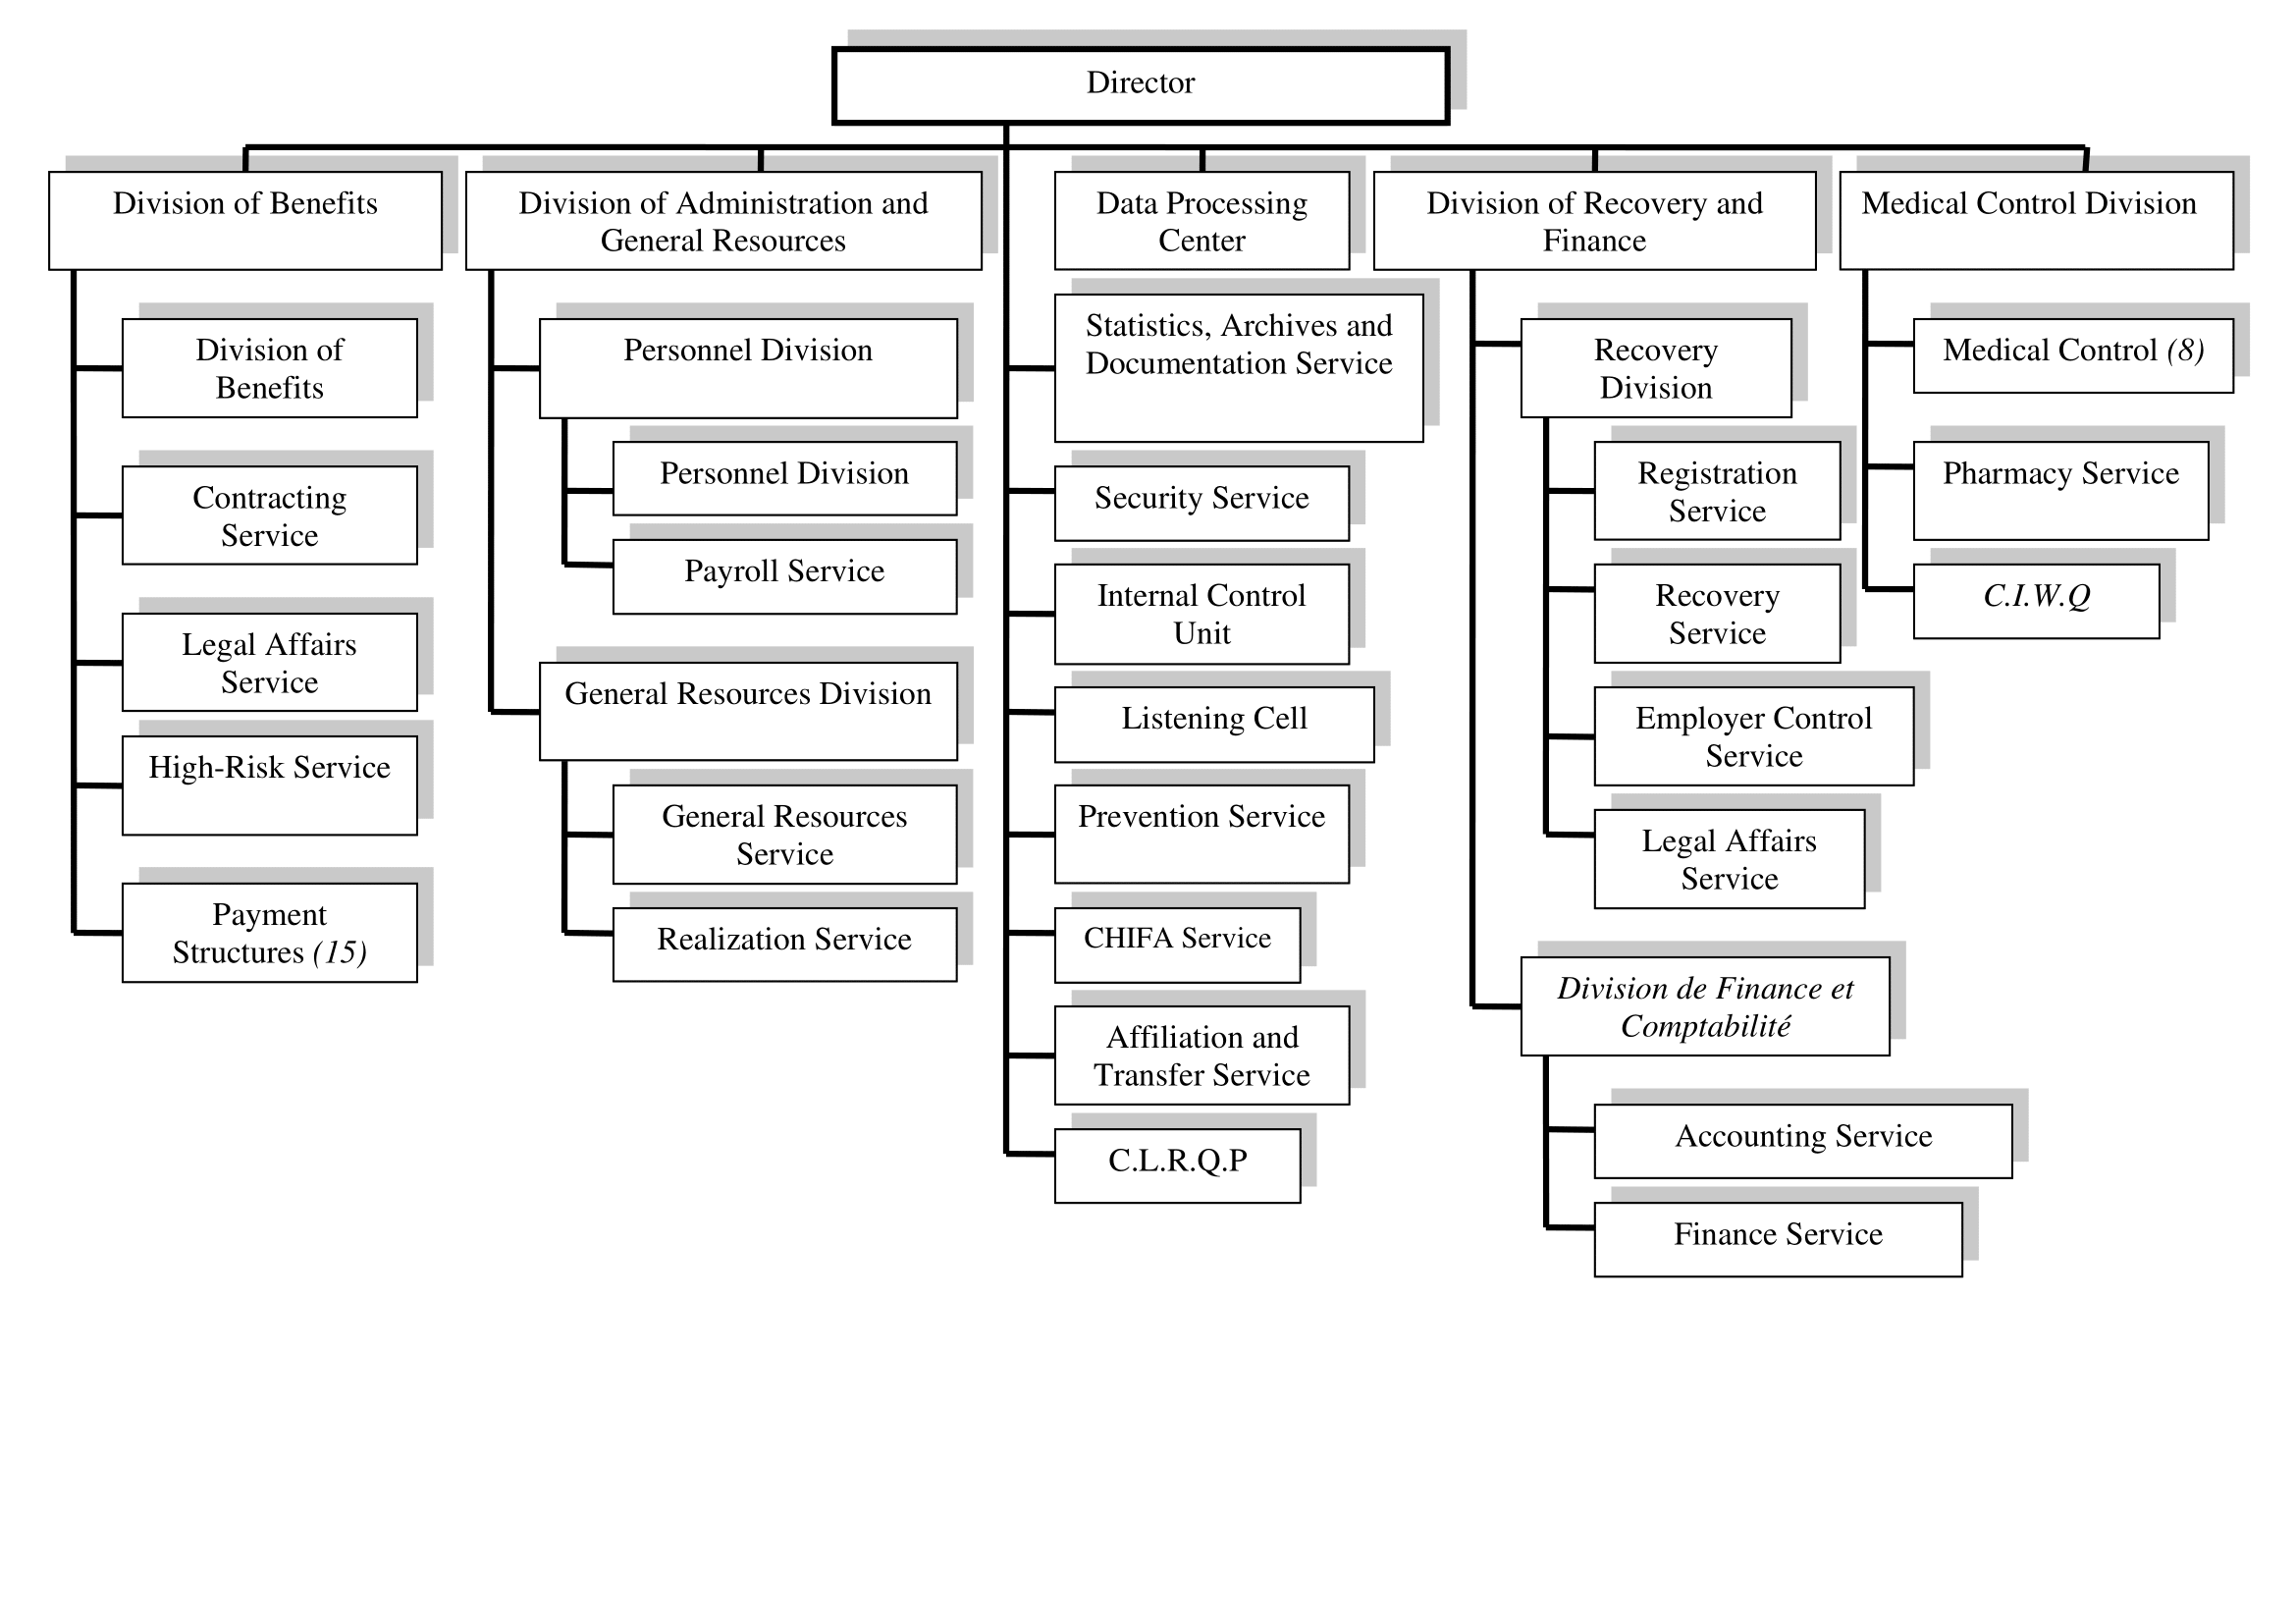
\includegraphics[width=1.0\textwidth]{organigram.png}
  \caption{Organigram of CNAS}
  \label{fig:organigram}
\end{figure}
\subsection{CNAS Services}
CNAS provides a range of services related to social security and healthcare to the Algerian population. These services include:
\begin{itemize}
    \item \textbf{Healthcare services:} CNAS operates its own specialized clinics and medical facilities, including four specialized clinics for cardiac surgery, orthopedics and rehabilitation, otorhinolaryngology, and dental care. It also runs 35 diagnostic and treatment centers, 55 pharmacies, and four regional medical imaging centers.

    \item \textbf{Social security services:} CNAS provides social security services to its members and their families, including health insurance, maternity leave benefits, disability benefits, and retirement pensions. It also offers services related to workplace safety and injury compensation.

    \item \textbf{Family services:} CNAS operates 30 nurseries and childcare centers to support working parents.

    \item \textbf{Payment services:} CNAS manages a network of payment centers and local correspondents to ensure the timely payment of social security benefits to its members.
\end{itemize}
\subsection{  Importance of CNAS services for the Algerian society}
These services are essential for the Algerian society, as they help provide access to healthcare and social security benefits to millions of people. CNAS's role in ensuring workplace safety and providing compensation for work-related injuries is also crucial in protecting the rights and wellbeing of workers across Algeria.

\section{Literature Review}
\label{sec:literature-review}

There has been a significant amount of research on the use of virtual counters in various contexts, including government services, healthcare, and banking.\footnote{Wang, Y., Wang, L., \& Wang, F. (2020). A review on virtual service counters. \textit{Journal of Service Science Research}, 12(1), 3-24.} Virtual counters have been found to offer several benefits, including improved efficiency, reduced wait times, and increased convenience for users.\footnote{Yao, Y., Yang, Q., \& Hu, Y. (2019). An evaluation of virtual counters in government services. \textit{International Journal of Public Administration}, 42(8), 708-721.}

One study found that virtual counters in government services were particularly effective in reducing wait times and improving the overall user experience.\footnote{Jia, J., \& Shi, Y. (2018). The impact of virtual service counters on customer satisfaction in government services. \textit{Public Administration Review}, 78(2), 239-250.} Another study focused specifically on virtual counters in healthcare and found that they could help reduce patient anxiety and improve the efficiency of healthcare services.\footnote{Liu, X., Li, Y., \& Chen, G. (2021). The impact of virtual service counters on patient satisfaction in healthcare. \textit{Journal of Healthcare Management}, 66(1), 24-34.}

In the banking industry, virtual counters have been used to provide personalized services to customers, such as financial advice and investment planning.\footnote{Zhu, Q., Chen, L., \& Fang, Y. (2019). The role of virtual service counters in enhancing customer satisfaction in the banking industry. \textit{International Journal of Bank Marketing}, 37(6), 1426-1442.} These services have been found to be effective in improving customer satisfaction and loyalty.
\subsection{Conclusion}
Overall, the literature suggests that virtual counters can offer significant benefits in a variety of contexts, including government services, healthcare, and banking. These benefits include improved efficiency, reduced wait times, and increased convenience for users. Based on this research, it is reasonable to expect that the implementation of a virtual counter system at CNAS could result in similar benefits for its users.

\section{Requirements analysis}
The requirements analysis phase identified several key features that the virtual counter for CNAS must provide. First, the system should provide a questionnaire for users to fill out, generating a checklist of necessary documents that must be obtained before the appointment. Second, it should allow users to book appointments online and provide them with a ticket number to avoid the need to wait in long queues. Third, it should allow CNAS staff to manage and monitor the appointments, including rescheduling or cancelling them if necessary. Fourth, the system should allow users to view their appointment history and provide feedback on their experience with the virtual counter. Finally, the system should ensure the security and privacy of all user data. 
\medskip 

These requirements will be used as a basis for the design, the conception and the implementation of the virtual counter system.

\section{Conclusion}
In this chapter, we have explored the current state of the art related to virtual counters, the organization of CNAS, and the literature review of virtual counters in various contexts. The use of virtual counters has been found to offer several benefits, including improved efficiency, reduced wait times, and increased convenience for users. CNAS, as an Algerian social security institution, provides a range of essential services to the Algerian society, including healthcare, childcare, and employment-related services.

Additionally, we have discussed the organization of CNAS and its numerous structures, such as its 49 Agences de wilaya and 826 structures de paiement. 
\medskip

Finally, we highlighted the importance of CNAS services for the Algerian society, emphasizing the need for modernization and innovation to ensure that these services continue to meet the evolving needs of its users.

Overall, this chapter provides a comprehensive understanding of the state of the art related to virtual counters and CNAS organization which serves as a foundation for the subsequent chapters in this dissertation.


\chapter{Conception}
\section{Purpose of the chapter}
The purpose of this chapter is to present the conception of a virtual counter system for the Algerian National Social Security Fund (CNAS). This chapter will provide a detailed explanation of the system design and architecture, database design, as well as the different diagrams and models used during the conception phase. The virtual counter system aims to improve the current management system used by CNAS by providing users with a more efficient and user-friendly way to gather necessary information and book appointments.
\section {Overview of the topics covered}
This chapter focuses on the conception of the virtual counter system for CNAS. It includes the analysis and design of the system, from the identification of user requirements to the development of the system architecture and database design. The chapter also includes the presentation of the different diagrams that were created, such as the use case diagram, class diagram, sequence diagram, and flowchart.
The aim of this chapter is to provide a comprehensive understanding of the virtual counter system, its components, and its functionalities.

\section{System design and architecture}
The system design and architecture of a virtual counter is a crucial aspect in developing a successful web application. It involves designing the components of the system and specifying how they interact with each other to achieve the desired functionality. In the case of a virtual counter for CNAS, the system design and architecture must take into account the different types of users, such as clients and agents, and the various tasks they need to perform. It must also ensure that the application is secure and reliable, with measures in place to protect user data and prevent unauthorized access. The system design and architecture will involve selecting suitable technologies and frameworks, such as Laravel and VueJs, and designing a database schema to store and retrieve data efficiently. Overall, a well-designed system architecture will contribute to the effectiveness and efficiency of the virtual counter and improve the user experience for both clients and agents.

\subsection{Description of the overall system architecture}
The overall system architecture of the virtual counter for CNAS is designed to be a web-based application with a client-server architecture. The client-side will be a user-friendly interface, developed using Vue.js framework, that allows users to interact with the system and perform different tasks, such as filling in a questionnaire that will generate a checklist of required documents, booking appointments, and checking their status. On the other hand, the server-side of the application will handle all the processing and data storage. It will be developed using the Laravel framework, which is a powerful and reliable PHP web application framework that enables rapid application development with a robust and scalable codebase. The application will also use a MySQL database to store all the necessary data, such as user information, appointment schedules, and queue status. The overall system architecture is designed to be modular and scalable, allowing for easy maintenance and future updates.
\newpage
\section{Diagrams illustrating the different components of the system}
Diagrams can help to provide a visual representation of the different components and processes involved in the virtual counter system, making it easier to understand and communicate to stakeholders.

\medskip The use of UML (Unified Modeling Language) which is a standered Language for visualizing and creating views to illustrate the different parts of a system , presenting us with a various types of diagrams that facilitates the conception phase for the virtual counter and makes it more comprehensive .  

\subsection{Use case diagram}
Use case diagram is one of the most used static diagrams in UML , it consist on explaining the different actions preformed by the user and helps understanding the main functions that can be preformed by the system.  

When the user is interacting with the system, the virtual counter enables him to consult the various services provided  by CNAS without the need to log in. 
 
 Additionally, the user can also complete a variety of tasks, such as selecting a service and completing a questionnaire related to that service. The system will then generate a checklist of the documents he will need to submit. The user can stop at printing that checklist or he can move on to booking an appointment which will require him to be authenticated. When an appointment is booked, an appointment ticket, that contains the previous checklist along with some appointment details such as the date and time, the counter number and the name of the employee responsible for treating your concerns,  will be available to print. 
 
 \medskip In the second hand of the virtual counter, both the employee and the supervisor have their own interactions with the system; however, in both their cases, they both need to be logged in order to access the various functionalities of the system. In addition to managing their work flow, both can manage the appointments by treating, rescheduling or canceling them if necessary. 
\newpage
 \medskip Here is the diagram:

 \begin{figure}[H]
    \centering
    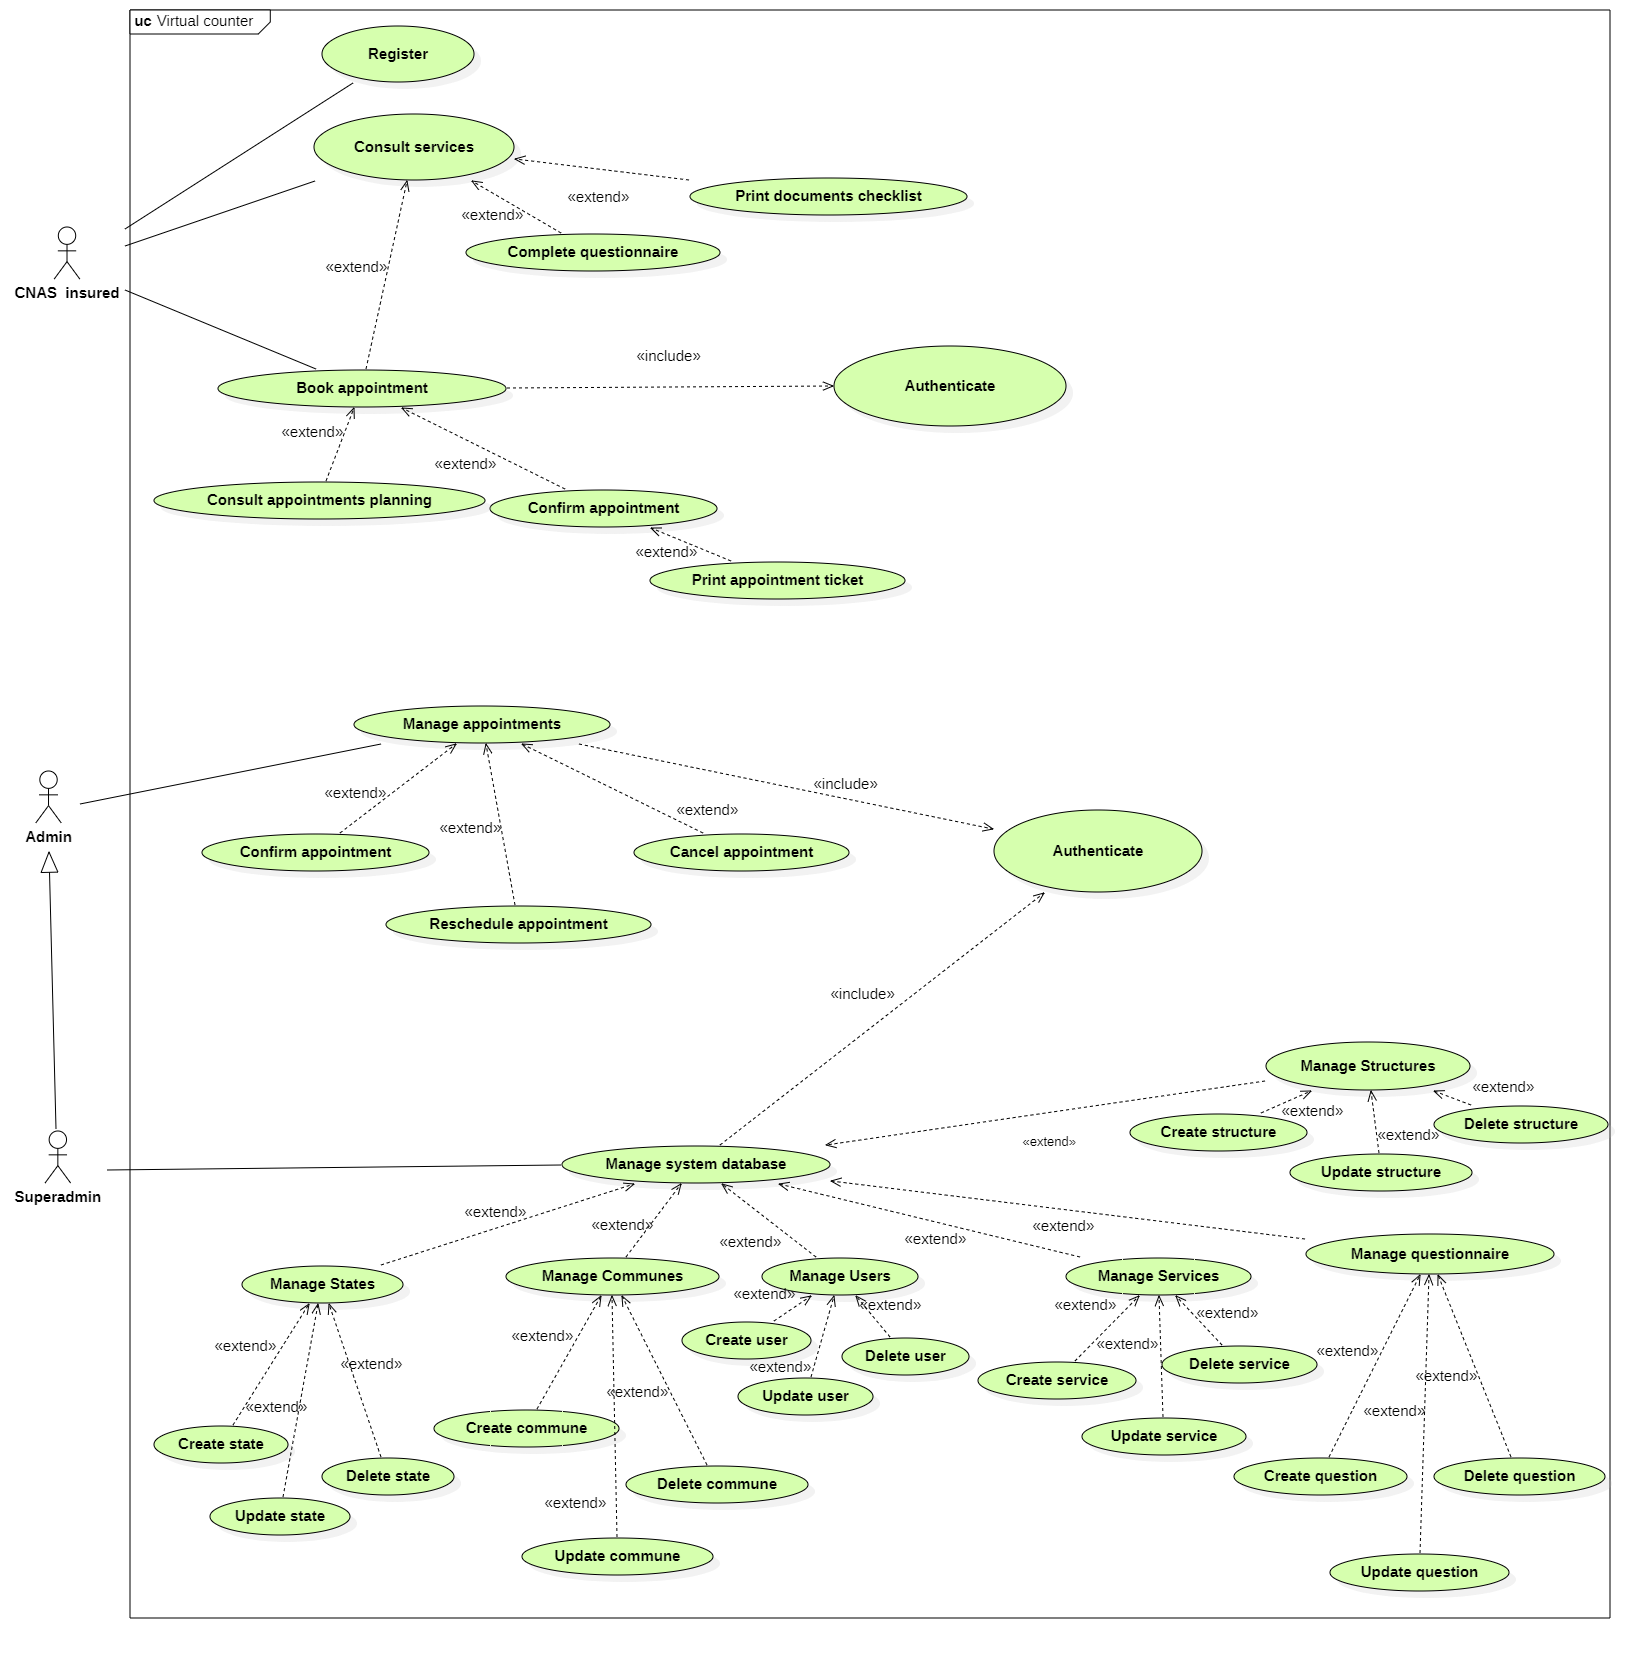
\includegraphics[width=1.0\textwidth]{UseCase.PNG}
    \caption{Use case diagram}
    \label{ucdiagram}
 \end{figure}
 \newpage
\subsection{Class diagram}
A class diagram is a type of UML diagram that represents the structure of a system by showing the classes, interfaces, and their relationships. It is an important tool for software engineers to design and communicate the architecture of a system. 

\medskip In this section, we present the class diagram of the CNAS virtual counter system. The diagram illustrates the key components of the system and their relationships, including the classes for managing users, services, appointments, and other relevant data. This diagram provides a visual representation of the system's architecture, which will help in understanding how the virtual counter works and how it can be further developed and maintained.

\bigskip Here's the class diagram:
\begin{figure}[H]
    \centering
    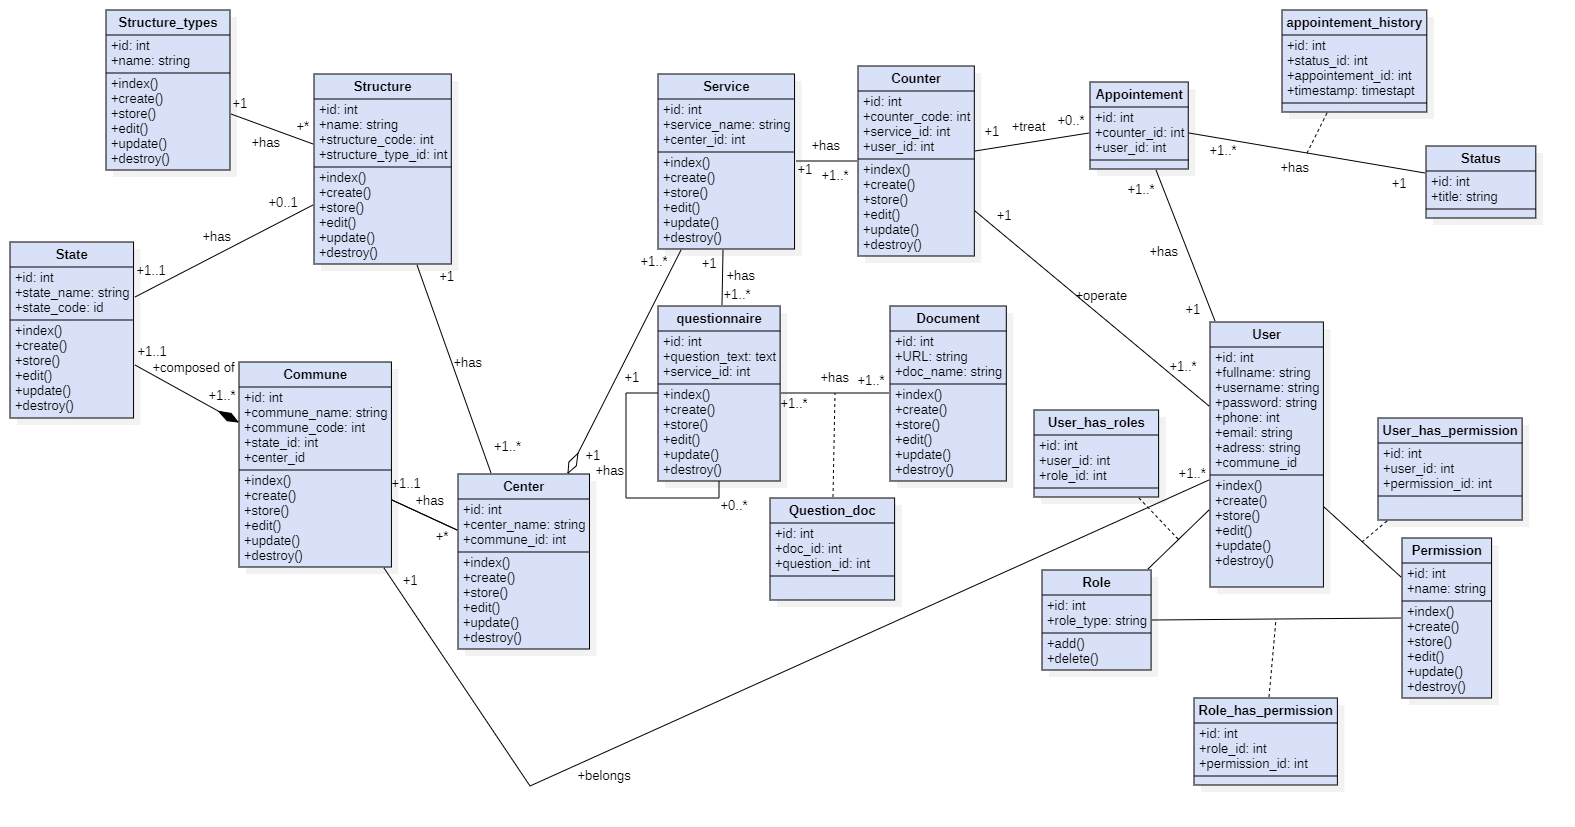
\includegraphics[width=1.0\textwidth]{ClassDiagram.png}
    \caption{Class diagram}
    \label{classdiagram}
\end{figure}
\newpage
\subsection{Sequence diagram}
Sequence diagram in one of the well known dynamic diagrams that allow the overall understanding for the hidden functionalities , and streamlines the developemnt phase . 

\medskip Here are the different diagrams related to every user in the application as well as the registration sytem . 
  \begin{figure}[H]
      \centering
      \includegraphics*[width=0.5\textwidth]{registration_sequence.PNG}
      \caption{Sequence diagram for Registration}
      \label{fig:Sequence diagram for Registration}
  \end{figure}
  \begin{figure}[H]
      \centering
      \includegraphics*[width=0.5\textwidth]{sequence_client.PNG}
      \caption{Sequence diagram for client interaction}
      \label{fig:Sequence diagram for Cient Interaction}
  \end{figure}
 
\subsection{Discussion of the design decisions made}
Overall, the decision discussions we had during the process of elaborating the UML diagrams helped us to refine the system's design and functionality and to ensure that it met the requirements and expectations of both the users and the organization. The final UML diagrams illustrate the system's architecture and behavior in a clear and concise manner, and provide a solid foundation for building a robust and efficient virtual counter system for CNAS.

\medskip We came to a final conception of the virtual counter on the basis of the notion of eliminating the waiting time in such an effective way and to ensure an efficient system, which can provide by far a great user experience and a sturdy system. 

\section{Database design}
At this juncture of conception, our primary focus was on creating a reliable database because a well-designed database is crucial for the efficient functioning of any application, including the virtual counter. We also made sure that accessing the data would be a secure process while also allowing stakeholders to track and store their data effectively.

\subsection{Overview of the database schema}
//
\subsection{Explanation of the different tables and their relationships}
//
\subsection{Discussion of the design decisions made}

//
\chapter{Implementation}
\section{Chapter Overview}
In this chapter, we will delve into the comprehensive implementation details of CNAS's virtual counter system. We will explore the utilization of various cutting-edge technologies that have played a pivotal role in the development process. Firstly, we will highlight the significance of Version Control Tool(VCS) GitHub, which facilitated seamless collaboration and ensured efficient code management throughout the project. Additionally, we will examine the utilization of the widely acclaimed PHP framework Laravel, known for its robustness and flexibility, which provided a solid foundation for building the web application. Furthermore, we will explore the integration of VueJs, a powerful JavaScript framework, that enabled us to develop an interactive and user-friendly interface. Together, these technologies synergistically contributed to the creation of a highly efficient and functional virtual counter system for CNAS.
\section{Development Tools and Technologies}
In the development of the virtual counter system, we utilized a set of powerful tools and technologies that contributed to its successful implementation. These tools played a crucial role in enhancing productivity, collaboration, and the overall performance of the system. Let's explore each of them briefly:

\begin{itemize}
  \item  
\includegraphics[height=2em]{Visual_Studio_Code_1.35_icon.svg.png} \textbf{VSCode (Visual Studio Code):} VSCode is a widely acclaimed source code editor known for its versatility and extensive plugin ecosystem. It provides a rich and intuitive development environment, offering features like intelligent code completion, debugging capabilities, and Git integration. Its flexibility and customizability make it a popular choice among developers.
  
  \item 
\includegraphics[height=2em]{github-logo.png} \textbf{GitHub:} GitHub is a web-based platform built on top of Git, enabling effective version control and collaboration. It provides a centralized repository for storing code, managing project milestones, and facilitating seamless collaboration among team members. GitHub's features, such as issue tracking, pull requests, and code reviews, streamline the development workflow and foster efficient teamwork.
  
  \item 
\includegraphics[height=2em]{1200px-Laravel.svg.png} \textbf{Laravel:} Laravel is a robust PHP framework that simplifies the development process by providing an elegant syntax and a wide range of built-in functionalities. With features like routing, ORM (Object-Relational Mapping), and template engine, Laravel enables rapid and scalable web application development. It promotes code reusability and follows the MVC (Model-View-Controller) architectural pattern.
  
  \item 
\includegraphics[height=2em]{Vue.js_Logo_2.svg.png} \textbf{Vue.js:} Vue.js is a progressive JavaScript framework that empowers the creation of interactive and dynamic user interfaces. Its component-based structure promotes code modularity and reusability, allowing for a more organized and maintainable codebase. Vue.js offers features like data binding, declarative rendering, and a rich ecosystem of libraries and plugins.
  
  \item 
\includegraphics[height=2em]{MariaDB_Logo.d8a208f0a889a8f0f0551b8391a065ea79c54f3a.png} \textbf{MariaDB:}  MariaDB is a popular open-source relational database management system derived from MySQL. It provides a reliable and scalable database solution with high performance and robust security features. With its SQL compatibility and extensive support for data manipulation and retrieval, MariaDB serves as the backbone for storing and managing the virtual counter system's data.
\end{itemize}

These tools and technologies synergistically contribute to the development of a powerful and efficient web-based application, ensuring a seamless User eXperience(UX) and streamlined management of the virtual counter system.

\section{Introduction to Git }
Software development involves managing a large number of files and assets that undergo frequent changes. As developers, we require a tool that facilitates the administration of these files and ensures consistent updates. This is where Git proves invaluable, providing us with the ability to handle such tasks with ease and flexibility. At its core, Git is a powerful tool that enables multiple individuals to collaborate on the same project while effectively tracking all changes made to the code and files over time.
\subsection{GitHub implementation}
In order to facilitate the development phase and ensure efficient version control for our virtual counter project, we have implemented GitHub. GitHub is a web-based platform that serves as a central repository for Git-based version control systems. It provides a range of tools and features that enable collaborative development, code management, and tracking of changes.

With GitHub, we have a centralized location where we can store and manage our project's codebase. It allows us to create and manage repositories, branches, and commits, making it easy to track changes and work on different features or bug fixes simultaneously. GitHub's version control capabilities ensure that we have a complete history of all modifications, allowing us to roll back changes if needed and maintain code integrity.

GitHub also offers collaborative features that enhance team collaboration and communication. We can create issues and assign them to team members, facilitating task management and bug tracking. Additionally, GitHub provides a platform for code review, allowing team members to review and provide feedback on each other's code, ensuring code quality and consistency.

By utilizing GitHub, we benefit from a robust and scalable infrastructure for our project's version control needs. It streamlines our development process, enables efficient collaboration, and ensures the traceability and integrity of our codebase.
\subsection{Advantages of Github in Development}
In this section, we will explore the advantages of utilizing GitHub in our development workflow. GitHub, as a powerful version control system and collaboration platform, offers a range of benefits that enhance the efficiency and effectiveness of our project.

\begin{itemize}
\item \textbf{Version Control:} GitHub allows for efficient and effective version control, enabling easy tracking of changes, branching, and merging of code. This ensures that the project's codebase is well-managed and allows for easy collaboration among team members.

\item \textbf{Collaboration and Teamwork:} GitHub provides a platform for seamless collaboration and teamwork. It allows multiple developers to work on the same project simultaneously, facilitating efficient communication, code sharing, and coordination of tasks. Features like pull requests and code reviews enhance collaboration and ensure high code quality.

\item \textbf{Code Integrity and History:} GitHub maintains a complete history of all code changes, making it easy to track modifications, roll back to previous versions if necessary, and maintain code integrity. This helps in identifying and resolving issues, ensuring a stable and reliable codebase.

\item \textbf{Project Management:} GitHub offers project management features such as issue tracking, task assignment, and milestone tracking. These tools streamline project management, enhance organization, and ensure that tasks are tracked and completed in a timely manner.

\item \textbf{Community and Open Source Collaboration:} GitHub has a large community of developers and provides a platform for open-source collaboration. It enables easy sharing of code, contribution to open-source projects, and learning from others in the community.
\end{itemize}
\subsection{GitHub Setup and Configuration}

In order to effectively utilize the features of GitHub for version control and collaboration, it is necessary to set up a GitHub account and configure Git on your local machine. This section provides step-by-step instructions on how to set up and configure GitHub, enabling you to seamlessly manage and contribute to your project repositories. Follow the steps below to get started:

\begin{enumerate}
    \item \textbf{Create a GitHub Account}: Begin by creating a GitHub account. Visit the GitHub website (\url{https://github.com}) and sign up for a new account. Provide the required information, such as your username, email address, and a secure password. Once registered, verify your email address to activate your GitHub account.
    
    \item \textbf{Install Git}: Proceed to install Git on your local machine if you haven't done so already. Git provides the necessary command-line tools to interact with GitHub repositories. Download the Git installer from the official website (\url{https://git-scm.com/downloads}) and follow the installation instructions for your operating system.
    
    \item \textbf{Configure Git}: After installing Git, configure your Git identity by setting your username and email address. Open the command-line interface (e.g., Terminal, Git Bash) and execute the following commands:
    
    \begin{verbatim}
    $ git config --global user.name "Your Name"
    $ git config --global user.email "your-email@example.com"
    \end{verbatim}
    
    These settings will be associated with your Git commits and will be visible in the commit history.
    
    \item \textbf{Generate SSH Key}: For secure interaction with GitHub repositories, it is recommended to generate an SSH key pair. Generate a new SSH key by executing the following command:
    
    \begin{verbatim}
    $ ssh-keygen -t rsa -b 4096 -C "your-email@example.com"
    \end{verbatim}
    
    Follow the prompts to specify the location for storing the key pair and provide a passphrase (optional but recommended). Once generated, add the SSH public key to your GitHub account by navigating to "Settings" -> "SSH and GPG keys" and adding the public key.
    
    \item \textbf{Configure Remote Repository}: If you are collaborating on an existing GitHub repository, clone the repository to your local machine using the following command:
    
    \begin{verbatim}
    $ git clone git@github.com:username/repository.git
    \end{verbatim}
    
    Replace \texttt{username} with your GitHub username and \texttt{repository} with the name of the repository. This command creates a local copy of the repository on your machine.
\end{enumerate}

By following these steps, you will have successfully set up and configured GitHub for your project, empowering you to effectively manage version control and collaborate with others in your development process.

\subsection{Github commands}
GitHub provides a powerful set of commands that enable efficient collaboration and version control in software development projects. These commands allow developers to clone repositories, create and manage branches, commit changes, push and pull code, merge branches, and initiate pull requests. Understanding these essential commands is crucial for effective GitHub usage and seamless teamwork. In this section, we will explore the key GitHub commands along with their descriptions and usage examples.

\medskip \begin{itemize}
    \item \textbf{Clone:} The \texttt{git clone} command allows you to create a local copy of a remote repository on your computer. For example: \texttt{git clone <repository URL>}.
  
    \item \textbf{Branch:} The \texttt{git branch} command is used to create, list, or delete branches in your repository. For example: \texttt{git branch <branch name>}.
  
    \item \textbf{Commit:} The \texttt{git commit} command is used to save changes made to your local repository. For example: \texttt{git commit -m "Commit message"}.
  
    \item \textbf{Push:} The \texttt{git push} command is used to upload local repository commits to a remote repository. For example: \texttt{git push origin <branch name>}.
  
    \item \textbf{Pull:} The \texttt{git pull} command is used to update your local repository with the latest changes from the remote repository. For example: \texttt{git pull origin <branch name>}.
  
    \item \textbf{Merge:} The \texttt{git merge} command is used to combine changes from different branches into the current branch. For example: \texttt{git merge <branch name>}.
  
    \item \textbf{Pull Request:} The \texttt{git pull request} command is used to propose changes from a branch to be merged into another branch. For example: \texttt{git pull request}.
  \end{itemize}

  \subsection{Collaboration and Teamwork}
GitHub provides powerful features that enable seamless collaboration and effective teamwork on software development projects. This section explores the various collaborative capabilities offered by GitHub, allowing multiple developers to work together efficiently and coordinate their efforts. From managing branches and pull requests to resolving conflicts and conducting code reviews, GitHub facilitates a collaborative environment that fosters teamwork and enhances productivity. This section demonstrates how to leverage these collaborative features to streamline the development process and maximize the effectiveness of your team.   

\subsection{Conclusion}
In this section, we explored the implementation of GitHub as a powerful collaboration and version control tool for our project. We discussed the setup and configuration process, essential commands for managing repositories, and the benefits of using GitHub for collaboration and teamwork. By leveraging GitHub's features such as branch management, pull requests, issue tracking, and project boards, we have enhanced our team's productivity and streamlined our development process. The use of GitHub has enabled us to effectively collaborate, track changes, and ensure the integrity of our codebase. With its robust features and user-friendly interface, GitHub has become an indispensable tool for our project's success.
\newpage
\section{Introduction to Laravel framework}
Laravel is one of the most well known web frameworks that is used widely among developers, it is an open-source PHP based framework that uses MVC (Modal-View-Controller) Architecture and offers various tool and features that allows developers to build high-quality applications with such an efficiency and quickness. 

\medskip Benefits of using Laravel for web development:
\begin{itemize}

\item \textbf{Expressive syntax: }Laravel offers an expressive and readable syntax that simplifies the process of writing code. It provides a wide range of functions and shortcuts that allow developers to accomplish complex tasks with minimal effort.

\item \textbf{MVC architecture: }Laravel follows the Model-View-Controller (MVC) architectural pattern, which promotes separation of concerns and enhances code organization. This architectural approach enables developers to create modular and maintainable applications.

\item \textbf{Powerful ORM: }Laravel's Eloquent ORM (Object-Relational Mapping) simplifies database operations by providing an intuitive and fluent interface to interact with databases. It allows developers to work with database records as objects, making database management and querying a breeze.

\item \textbf{Robust routing system: }Laravel's routing system allows developers to define clean and flexible routes for their web applications. It supports various HTTP methods, route parameters, and route grouping, making it easy to handle complex URL structures.

\item \textbf{Blade templating engine: }Laravel's Blade templating engine offers a concise and powerful way to create dynamic views. It provides features like template inheritance, control structures, and reusable components, enabling developers to build modular and reusable UI components.

\item \textbf{Authentication and authorization: }Laravel simplifies user authentication and authorization processes with built-in functionalities. It provides secure user registration, login, and password reset mechanisms, as well as fine-grained access control using gates and policies.

\item \textbf{Rich ecosystem and community support: }Laravel has a vibrant and active community of developers who contribute to its growth. The framework benefits from a vast ecosystem of packages and libraries that extend its capabilities, allowing developers to leverage existing solutions and accelerate development.

\item \textbf{Testing and debugging tools: }Laravel provides robust testing and debugging tools that help developers ensure the quality and reliability of their applications. It supports unit testing, feature testing, and includes convenient debugging tools for efficient troubleshooting.
\end{itemize}

\medskip Overall, Laravel is an excellent choice for building web applications of any size and complexity, the choice of implementing this particular framework has been proven to be a wise decision, and that's due to its powerful set of tools an features that enabled us to create a robust and scalable web application that meets the needs of CNAS and its users. 
\section{Laravel implementation}
\subsection{Installation and setup}
In this section we will discuss the installation guide for laravel and its different components. In order to install and setup laravel correctly and without any issues, there is some requirements needs to be fulfilled in case of not using the homestead virtual machine. 
\cite{laravel} 

\medskip These requirements are: 

\begin{itemize}
    \item PHP version 7.2.5 or greater. 
    \item BCMath PHP Extension
    \item Ctype PHP Extension
    \item Fileinfo PHP extension
    \item JSON PHP Extension
    \item Mbstring PHP Extension
    \item OpenSSL PHP Extension
    \item PDO PHP Extension
    \item Tokenizer PHP Extension
    \item XML PHP Extension \footnote{Laravel. Laravel Documentation. Retrieved from \url{https://laravel.com/docs/7.x} }
\end{itemize}
 \medskip If the previous requirements are validated, we then move on to the installation guide for laravel, to do so it is highly recommended to follow the steps listed.
 \begin{enumerate}
\item \textbf{Install Laravel and its dependencies:}
  
Ensure that you have PHP installed on your system. Laravel requires PHP 7.4 or higher.
  
Install Composer, a dependency manager for PHP, if you haven't already. Composer is used to install Laravel and manage its dependencies.
  Open a terminal or command prompt and run the following command to install Laravel globally on your system:
   \begin{verbatim}
    composer global require laravel/installer
   \end{verbatim}
   

\item \textbf{Configure the development environment:}
  
Laravel requires a web server and a database to run. You can use popular web servers like Apache or Nginx, along with databases like MySQL or SQLite.
  
Ensure that your web server and database server are properly installed and configured. If needed, consult their respective documentation for installation and setup instructions.
\newpage
\item \textbf{Initialize a new Laravel project:}
 
Once Laravel is installed and your development environment is set up, you can create a new Laravel project.
  
Open a terminal or command prompt and navigate to the directory where you want to create your project.
  Run the following command to create a new Laravel project:
   \begin{verbatim}
    laravel new your-project-name 
   \end{verbatim}
   
   Replace "your-project-name" with the desired name for your project. This command will create a new directory with the specified project name and install the necessary files and dependencies.

\item \textbf{Test your installation:}
  
Change into the project directory:
\begin{verbatim}
    cd your-project-name
\end{verbatim}
   
Start the local development server by running the following command:
\begin{verbatim}
    php artisan serve
\end{verbatim}
  By default, the development server will start on (\url{http://localhost:8000}) 
  
  Open your web browser and visit that URL. If you see the Laravel welcome page, it means your installation was successful. 
  \item \textbf{PHP configuration:}
  
  Open the PHP configuration file (php.ini) on your system. The location of this file may vary depending on your operating system and PHP installation.
 
  Ensure that the following PHP extensions are enabled by uncommenting their respective lines (remove the semicolon ";" at the beginning of the line if present):
 \begin{verbatim}
    extension=fileinfo
    extension=openssl
    extension=pdo_mysql
 \end{verbatim}
 \newpage
 \item \textbf{Creating the ".env " file :}

 Laravel comes with a `.env.example' file by default. 
 \begin{itemize}
    \item 
    Make a copy of this file and rename it to `.env' by running the following command:
    \begin{verbatim}
       cp .env.example .env 
    \end{verbatim}
    \item Setting up the environment variables:
     
    Open the `.env' file in a text editor.

    Update the variables according to your development environment. For example, you might need to set the database credentials:
\begin{verbatim}
    DB_CONNECTION=mysql
    DB_HOST=127.0.0.1
    DB_PORT=3306
    DB_DATABASE=your_database_name
    DB_USERNAME=your_database_username
    DB_PASSWORD=your_database_password
\end{verbatim}

You can also configure other variables like the application URL, mail settings, caching drivers, and more. Refer to the comments in the `.env.example' file or Laravel's documentation for more information on available options.
\end{itemize}
\item \textbf{Generating the application key: }

Laravel requires an application key for secure encryption and other purposes. 

Run the following command to generate the key:
\begin{verbatim}
php artisan key:generate
\end{verbatim}
\item \textbf{Protecting sensitive information:}

   Ensure that the .env file is not publicly accessible. It should be kept outside of your version control system or any public directories.
    
   If you deploy your application to a production server, you may need to set the environment variables directly on the server or through the server's configuration management tools.
 \end{enumerate}
\subsection{Laravel directory structure}

In a Laravel project, the directory structure is designed to provide a clear organization for your application's files. Understanding the key directories and files will help you navigate and manage your Laravel project effectively. Here's an explanation of the purpose of each directory and some important files:
\begin{itemize}
    \item \textbf{app:}
        Contains the core application code, including controllers, models, and other PHP classes specific to your application's domain logic.

    \item \textbf{bootstrap:}
        Contains the files responsible for bootstrapping the Laravel framework and initializing the application environment.

    \item \textbf{config:}
        Contains configuration files for various aspects of your application, such as database connections, caching, mail settings, and more.

    \item \textbf{database:}
        Contains database-related files, including migrations for managing database schema changes, seeders for populating the database with sample data, and factories for generating test data.

    \item \textbf{public:}
        The web server's document root should be set to this directory. It contains the entry point for your application (index.php) and serves as the public-facing directory for static assets, such as CSS, JavaScript, and image files.

    \item \textbf{resources:}
        Contains views, language files, and frontend assets used by your application.
        views: Contains the Blade templates that define the UI of your application.
        lang: Contains language files for localization and internationalization.
        assets: Contains frontend assets, such as CSS, JavaScript, and images, that will be compiled and optimized by Laravel Mix.

    \item \textbf{routes:}
        Contains route definition files that specify how incoming requests should be handled by your application.
        web.php: Defines routes for web-based endpoints.
        api.php: Defines routes for API endpoints.
        You can create additional route files for organizing routes based on specific functionalities or modules.

    \item \textbf{storage:}
        Contains files generated by your application, such as logs, cached views, and uploaded files.
        app: Contains files generated by your application, such as cached config files, logs, and other temporary files.
        framework: Contains framework-generated files, including cached views, sessions, and routes.
        logs: Contains log files generated by your application.

    \item \textbf{tests:}
        Contains test files and directories for automated testing of your application.
        Feature: Contains feature tests, which test the application's behavior from the user's perspective.
        Unit: Contains unit tests, which test individual components of your application in isolation.

    \item \textbf{.env:}
        The environment file that holds environment-specific configuration values for your application.
        Contains settings such as database connections, mail configurations, and environment variables.
        It's important to keep this file secure and not expose any sensitive information.

    \item \textbf{composer.json and composer.lock:}
        These files manage the project's dependencies using Composer, a PHP dependency manager.
        composer.json lists the project's dependencies and defines autoloading rules.
        composer.lock locks the versions of the dependencies to ensure consistent installations.

    \item \textbf{artisan:}
        The command-line interface (CLI) tool for executing various commands within your Laravel application.
        Allows you to run tasks such as running migrations, generating code, and running tests.
\end{itemize}
Understanding the purpose of each directory and file in a Laravel project will help you navigate and locate the appropriate locations for adding or modifying code, configurations, and assets. It's important to maintain the integrity of the directory structure while organizing your code and assets within the appropriate directories.
\subsection{Routing}

Routing is an essential aspect of web development, and Laravel provides a powerful and flexible routing system. Here's an explanation of routing in Laravel, including how to define routes, work with route parameters, and utilize route grouping and naming.

Routing in Laravel refers to the process of mapping incoming HTTP requests to specific actions or handlers within your application. It determines how different URLs are handled and defines the endpoints through which users can access various functionalities of your application.

In Laravel, routes are typically defined in the `routes` directory, specifically the `web.php` and `api.php` files.
\begin{enumerate}
    \item \textbf{Basic route definition:} 
    
    A basic route is defined using the `Route` facade's methods, such as `get`, `post`, `put`, `patch`, and `delete`.
    
    \medskip Here's an example of a basic route definition:
    \begin{verbatim}
        Route::get('/home', function () {
            return 'Welcome to the home page!';
            });       
         \end{verbatim}
     
   This route responds to the `GET` request to the `/home` URL and returns the specified message.

 \item \textbf{Route parameters:}
   You can define routes with parameters that are passed as segments in the URL.
   
   \medskip Here's an example of a route with a parameter:
     \begin{verbatim}
        
        Route::get('/users/{id}', function ($id) {
            return 'User ID: ' . $id;
            });
        \end{verbatim}

    This route matches URLs like `/users/1`, `/users/2`, etc., and the parameter `{id}` is passed to the route closure as an argument.

\item \textbf{Route grouping and naming:}

Laravel allows you to group related routes and assign names to them for easy referencing and organization.
\begin{itemize}
    \item \textbf{Route grouping:}
    
    Route grouping allows you to apply common attributes or middleware to a group of routes.
    
    \medskip Here's an example of route grouping with a shared middleware:
\begin{verbatim}
    
        Route::middleware('auth')->group(function () {
            Route::get('/dashboard', function () {
                return 'Welcome to the dashboard!';
                });
                Route::get('/profile', function () {
                    return 'Welcome to your profile!';
                    });
                    });
                    
    \end{verbatim}
   In this example, the routes `/dashboard` and `/profile` are grouped together and share the `auth` middleware, which ensures that only authenticated users can access them.

    \item \textbf{Route naming:}
   
    Assigning names to routes helps in referencing them within your application, such as generating URLs or redirecting to specific routes.
    
    \medskip Here's an example of naming routes:
    \begin{verbatim}
        
        Route::get('/posts', function () {
            return 'List of posts';
            })->name('posts.index');
            
            Route::get('/posts/{id}', function ($id) {
                return 'Post ID: ' . $id;
                })->name('posts.show');
            \end{verbatim}
                
            In this example, the routes `/posts` and `/posts/{id}` are named as `posts.index` and `posts.show`, respectively. These names can be used later to generate URLs or redirect to these routes.
            
            By understanding and utilizing routing in Laravel, you can define the endpoints for your application, handle various HTTP methods, work with dynamic route parameters, group related routes, and assign names for easy referencing. Laravel's routing system provides the flexibility and convenience required to build robust and maintainable web applications.
        \end{itemize}
 \end{enumerate}
\subsection{Controllers}

Controllers play a crucial role in Laravel applications as they handle the logic and actions associated with different routes. Here's an explanation of creating and using controllers in Laravel, defining controller methods and actions, and understanding the separation of concerns between routes and controllers.

The creation of an controller is done by the following artisan command: 
\begin{verbatim}
   php artisan make:controller
\end{verbatim}

For instance, to create the user controller we used the following command: 
\begin{verbatim}
    php artisan make:controller UserController 
\end{verbatim}

This command will generate a new `UserController` class in the `app/Http/Controllers` directory, which will be and empty class. 

In order to use the controller we must define its methods, it represent the actions that can be performed on a resource. These methods are responsible for processing requests, interacting with models or other methods, and returning appropriate responses and views.

\medskip Here is an example of the controller created in our application:
\begin{verbatim}
    namespace App\Http\Controllers;

     class UserController extends Controller
     {
         public function index()
         {
             // Retrieve users from the database
             $users = User::all();

             // Return a view with the users
             return view('users.index', compact('users'));
         }

         public function show($id)
         {
             // Retrieve a specific user from the database
             $user = User::findOrFail($id);

             // Return a view with the user details
             return view('users.show', compact('user'));
         }
     }
\end{verbatim}
\begin{itemize}
    \item \textbf{Assigning controller to route:}
    
    \medskip Controllers and Routes are two highly related components in the application system, that's why we need to make them communicate with each other and that's by Assigning the controllers to the specific appropriate routes, the following step show how that can be done.
    
    To assign a controller to a specific route, we move to the routes directory, specifically in the 'web.php' file and create the following code:
    \begin{verbatim}
        use App\Http\Controllers\UserController;
        
        Route::get('/users', [UserController::class, 'index']);
        Route::get('/users/{id}', [UserController::class, 'show']);
    \end{verbatim}
    In this example, the `index` method of the `UserController` will be executed when the `/users` route is accessed, and the `show` method will be executed for `/users/{id}`.

    Laravel also provides a more expressive syntax using the `Route::controller` method to bind all routes for a controller automatically. and that's by using the resource tag.
\item \textbf{Separation of concerns between routes and controllers:}

Laravel follows the principle of separation of concerns, where routes and controllers have distinct responsibilities:

\begin{enumerate}
    \item \textbf{Routes:}
    
    Routes define the URL patterns and HTTP methods that trigger specific actions in your application,
    they provide a mapping between incoming requests and the appropriate controller method or closure.
   
    Routes are responsible for handling the request lifecycle, middleware application, and route-specific logic.
    \item \textbf{Controllers:}
    
     Controllers encapsulate the application logic related to processing requests and generating responses,
     They handle the business logic, interact with models or services, and prepare the data to be presented to the user using views.
    
     Controllers promote code reusability and maintainability by keeping the route definitions concise and focused on routing concerns.
\end{enumerate}
By separating routes and controllers, you achieve a clean and modular structure for your application. Routes define the endpoints and how to handle them, while controllers centralize the related logic and actions. This separation promotes code organization, improves maintainability, and allows for easier testing and reuse of controller methods across different routes.
\end{itemize}

\medskip Using controllers in Laravel helps you manage the complexity of your application, adhere to the principles of MVC architecture, and ensure a clear separation of concerns between different components of your application.
\subsection{Views and Blade templates}
   
Views and Blade templates are crucial components in Laravel that handle the presentation layer of your application. They allow you to separate the UI (User-Interface) logic from the rest of your code and provide a flexible way to generate and render HTML. In this section we will delve into the explanation of views and templates in Laravel, including creating and rendering views, and working with the Blade templating engine.
\begin{itemize}
    \item \textbf{views and templates:}
    
    Views in Laravel are responsible for presenting the data to the user. They contain the HTML markup, CSS styles, and placeholders where dynamic data can be inserted. Templates, on the other hand, are reusable layouts that define the overall structure and common elements of multiple views.
    \item \textbf{Creating and rendering view:}
    \begin{enumerate}
        \item \textbf{Creating the view:}
        
        Views are typically stored in the `resources/views` directory, to create a view, you can simply create a new Blade template file with the `.blade.php` extension.
        \item \textbf{Rendering a view:}
        
        To render a view, you can use the `view` helper function or the `View` facade.
        
        Here's an example of rendering the `welcome` view:
        \begin{verbatim}
            return view('welcome');
        \end{verbatim}
        This code will locate and render the `welcome.blade.php` view file.
        \item \textbf{Passing data to views:}
        
        You can pass data from your controller to the view by chaining the `with` method or using the second argument of the `view` function.
        Here's an example of passing data to the view:
        \begin{verbatim}
            $user = User::find(1);
            return view('profile')->with('user', $user);
        \end{verbatim}
        In the `profile.blade.php` view, you can access the "user" variable.
     \end{enumerate}
     \item \textbf{Working with Blade templating engine:}
     \begin{enumerate}
        \item \textbf{Blade syntax:}
        
        Blade provides a convenient and expressive syntax for working with views.
        
        For example, you can use the `{{ }}` syntax to echo variables or the `@if`, `@foreach`, and `@endif` directives for conditional statements and loops.
        \item \textbf{Blade directives:}
        
        Blade offers several directives to enhance the templating experience.
        
        Examples of directives include:
         
        `@extends('layout')`: Specifies that the view extends a layout template.
        
        `@section('content')`: Defines a section within the view.
        
        `@yield('content')`: Renders the content of a section defined in the layout.
        
        `@include('partial')`: Includes a partial view.
        
        `@if`, `@else`, `@elseif`, `@endif`: Conditionally execute code.
        
        `@foreach`, `@endforeach`: Iterate over a collection.
    
        \item \textbf{Layouts and master templates:}
        
        Layouts allow you to define the common structure and elements shared across multiple views, typically, a layout template contains the HTML structure, header, footer, and placeholders for dynamic content, by extending a layout, you can inject specific content into the predefined sections.
        
        Here's an example of a layout template named `layout.blade.php`:
        \begin{verbatim}
            <!DOCTYPE html>
     <html>
     <head>
         <title>@yield('title')</title>
     </head>
     <body>
         <header>
             <!-- Common header content -->
         </header>

         <div class="content">
             @yield('content')
         </div>

         <footer>
             <!-- Common footer content -->
         </footer>
     </body>
     </html>
        \end{verbatim}
    \end{enumerate}
\end{itemize}
By utilizing views and Blade templates in Laravel, we could achieve a clean separation of concerns between the user interface and other application like conntrollers and its methods.
\subsection{Models and Eloquent ORM}
\begin{itemize}
 \item \textbf{Models:}

Models are used to represent the data and business logic of a web application, it allows developers to interact with the application's database in a more intuitive and object-oriented way, rather than writing raw SQL queries.

In the context of the CNAS virtual counter, models would be used to represent the various entities in the system, such as users, appointments, and requests. For example, a User model might represent the attributes and behavior of a user in the system, such as their name, email, and username.

To create a model in Laravel, we used the Artisan command-line tool to generate a new class that extends Laravel's base Model class. This new class represents a table in the application's database, and includes methods for interacting with the table's data.

For example, to create a User model we use the artisan command : 
\begin{verbatim}
    php artisan make:model User
\end{verbatim}
This generates a new User.php file in the "app" directory of the Laravel project, which contains the basic structure of a model class, we can add new methods if needed .

The overall structure of a modal is : 
\begin{verbatim}
    class User extends Model
    {
        public function posts()
        {
            return $this->hasMany(Post::class);
        }
    }

    class Post extends Model
    {
        public function user()
        {
            return $this->belongsTo(User::class);
        }
    }
\end{verbatim}
\item \textbf{Eloquent ORM: }

In Laravel, Eloquent ORM (Object-Relational Mapping) is the default database system used to interact with database tables and records. Eloquent provides a simple and intuitive way to interact with database tables using PHP code, making it easier and more efficient to work with data in a Laravel application.

Some of the most commonly used Eloquent methods include:
\begin{itemize}
     
    \item \textbf{all()} - Retrieves all records from a database table.
    
    \item \textbf{find()} - Retrieves a single record from a database table by its primary key.
    
    \item \textbf{create()} - Inserts a new record into a database table.

    \item \textbf{update()} - Updates one or more records in a database table.

    \item \textbf{delete()} - Deletes one or more records from a database table.

    \item \textbf{where()} - Filters records based on specific criteria.

    \item \textbf{orderBy()} - Sorts records based on a specific field.

    \item \textbf{limit()} - Limits the number of records returned by a query.

    \item \textbf{join()} - Joins multiple tables together in a query.

    \item \textbf{select()} - Specifies which fields to include in a query result.
\end{itemize}
In addition to these basic methods, Eloquent also provides many more advanced features, such as relationships between tables. 

There are four types of relationships: one-to-one, one-to-many, many-to-one, and many-to-many. Each relationship type can be defined using methods on the model class that corresponds to the related table.
\begin{itemize}
    \item \textbf{One-to-One Relationship:}
    
    In a one-to-one relationship, a record in one table is related to exactly one record in another table. For example, a user might have a single profile record that contains additional information about the user. In Eloquent, a one-to-one relationship can be defined using the "hasOne" and "belongsTo" methods.
    \item \textbf{One-to-Many Relationship:}
    
    In a one-to-many relationship, a record in one table can be related to many records in another table. For example, a user might have many posts in a blog application. In Eloquent, a one-to-many relationship can be defined using the "hasMany" and "belongsTo" methods.
    \item \textbf{Many-to-One Relationship:}
    
    A many-to-one relationship is essentially the opposite of a one-to-many relationship. In a many-to-one relationship, many records in one table can be related to a single record in another table. For example, many posts might belong to a single user in a blog application. In Eloquent, a many-to-one relationship can be defined using the "belongsTo" and "hasMany" methods.
    \item \textbf{Many-to-Many Relationship:}
    
    In a many-to-many relationship, many records in one table can be related to many records in another table. For example, a user might have many roles in an application, and each role might be associated with many users. In Eloquent, a many-to-many relationship can be defined using the "belongsToMany" method.
\end{itemize}
After implementing those relations on the application tables, now we can retrieve data from multiple tables with one function seamlessly and with ease, by using with() function.

This feature reduces the number of database queries required to retrieve data and improves the performance of the application.
\end{itemize}
Overall, Eloquent ORM offers a full range of techniques and capabilities that make working with database tables and records in a Laravel application simple and effective. we can create code that is easier to comprehend, extend over time, and is cleaner, more maintainable, and more extensible by utilizing Eloquent to communicate with the database.
\subsection{Database Migrations and Seeders}
Database migrations and seeding are important aspects of Laravel that help in managing the database schema and populating it with sample or test data. 

Here's an explanation of Laravel's database migrations, including creating and running migrations, as well as seeding the database with sample data.

Database migrations in Laravel provide a version control system for your database schema. They allow you to define and modify the structure of your database using PHP code, making it easy to collaborate with other developers and maintain consistency across different environments.
\begin{enumerate}
\medskip \item \textbf{Creating and running migrations:}
\begin{enumerate}
    

\item \textbf{Creating a migration:}
   
- You can create a new migration using the `make:migration` Artisan command. 
   
   For example, to create a migration for creating a `users` table, run the following command:
   \begin{verbatim}
     php artisan make:migration create_users_table --create=users
   \end{verbatim}
   - This command will generate a new migration file in the `database/migrations` directory.

\item \textbf{Defining the migration:}
   
- Open the generated migration file and use the available methods like `up` and `down` to define the changes to be made to the database.
   - For example, in the `up` method, you can use the `Schema` facade to create tables, add columns, define indexes, or set foreign key constraints.
   - Here's an example of a migration for creating a `users` table:
\begin{verbatim}
     use Illuminate\Database\Migrations\Migration;
     use Illuminate\Database\Schema\Blueprint;
     use Illuminate\Support\Facades\Schema;

     class CreateUsersTable extends Migration
     {
         public function up()
         {
             Schema::create('users', function (Blueprint $table) {
                 $table->id();
                 $table->string('name');
                 $table->string('email')->unique();
                 $table->timestamps();
             });
         }

         public function down()
         {
             Schema::dropIfExists('users');
         }
     }
\end{verbatim}

\item \textbf{Running migrations:}
   
- To run migrations and apply the changes to the database, use the `migrate` Artisan command:
   \begin{verbatim}
     php artisan migrate
    \end{verbatim}
   - This command will execute any pending migrations and update the database schema accordingly.
\end{enumerate}

\item \textbf{Seeding the database with sample data:}

\medskip Database seeding allows you to populate your database with sample or test data. Laravel provides a convenient way to define seeders and run them to insert data into your database.
\begin{enumerate}
    \item \textbf{Creating a seeder:}
   
    - You can create a new seeder using the `make:seeder` Artisan command. For example, to create a seeder for generating sample users, run the following command:
   \begin{verbatim}
     php artisan make:seeder UserSeeder
    \end{verbatim}
   - This command will generate a new seeder file in the `database/seeders` directory.

   \item \textbf{Defining the seeder:}
   
   - Open the generated seeder file and use the `run` method to define the data to be inserted into the database.
   - You can use Eloquent models or plain database queries to create and insert records.
   - Here's an example of a seeder for creating sample Role types:
\begin{verbatim}
     use Illuminate\Database\Seeder;
     use App\Models\User;

     class RolesTableSeeder extends Seeder
     {
         public function run()
         {
             $roles = [
                 'superadmin',
                 'manager',
                 'admin',
                 'user',
                 'superviseur',
             ];
             foreach ($roles as $role) {
                 Role::create(['name' => $role]);
             }
         }
     }
\end{verbatim}

\item \textbf{Running seeders:}
   
- To run the seeders and populate the database with sample data, use the `db:seed' Artisan command:
   \begin{verbatim}
     php artisan db:seed
    \end{verbatim}
   - This command will execute all the seeders that you have defined. By default, it will run all the seed classes located in the database/seeders directory.

  \medskip However, if you want to run a specific seeder class, you can use the --class option followed by the seeder class name. For example:
   
    \begin{verbatim}
   php artisan db:seed --class=UserSeeder
    \end{verbatim}
   This command will execute only the UserSeeder class, seeding the database with the defined sample user data.
   
   Alternatively, you can use the --seed option to specify a specific seeder file to run:
   \begin{verbatim}
    php artisan db:seed --seed=users
    \end{verbatim}
   - This command will execute the users seeder file specifically.
   
   You can choose to run all seeders or target specific seeders based on your requirements.
\end{enumerate}   
\end{enumerate}
\subsection{Form Handling and Validation}
Form handling and validation are essential for processing user input in web applications. Laravel provides convenient features for handling form submissions, validating user input, and displaying validation errors. 

\medskip Here's an explanation of form handling and validation in Laravel:
\begin{itemize}
    \item \textbf{Handling form submissions in Laravel:}
\begin{enumerate} 
    \item \textbf{Defining a form:}
   - Create an HTML form using the `\textless form\textgreater' element in your view.
   - Set the form's `action' attribute to the appropriate route that will handle the form submission.
   - Specify the form's `method' attribute as `POST' to send the form data securely.

   \item \textbf{Route for form submission:}
   - Define a route that corresponds to the form's `action' attribute.
   - In the route definition, specify the controller method or closure that will handle the form submission.

   \item \textbf{Processing the form submission:}
   - In the controller method or closure, you can access the submitted form data using the `request' helper or by type-hinting the \textbf{`Illuminate\textbackslash Http\textbackslash Request'} class.
   - You can then perform the necessary operations, such as saving data to the database or sending email notifications.
\end{enumerate} 
   \item \textbf{Validating user input using Laravel's validation rules:}
   \begin{enumerate}
    \item \textbf{Defining validation rules:}
   - Laravel provides a fluent validation system for validating user input.
   - In the controller method or closure that handles the form submission, you can define validation rules using the `validate' method.
   - The validation rules define the expected format and constraints for each form field.
   - For example, you can specify that a field is required, must be an email, or must be a specific length.

   \item \textbf{Validating the input:}
   - Call the `validate' method on the incoming request to validate the user input against the defined rules.
   - If the validation fails, Laravel will automatically redirect back to the form with the validation errors.
\end{enumerate} 
   \item \textbf{Displaying validation errors to the user:}
   \begin{enumerate}
    \item \textbf{Redirecting back with errors:}
   - When the validation fails, Laravel will redirect the user back to the form with the validation errors flashed to the session.
   - You can use the `withErrors' method when redirecting back to store the validation errors in the session.

   \item \textbf{Displaying errors in the view:}
   - In the form view, you can use the `@error' directive to display specific validation errors for a field.
   - The `@error' directive checks if there are errors for a given field and displays the corresponding error message if available.
\end{enumerate} 
\end{itemize}
\subsection{Authentication and Authorization}
Authentication and authorization are crucial aspects of web applications. Laravel provides a comprehensive system for implementing user authentication and managing access control. Here's an explanation of authentication and authorization in Laravel, including user registration, login, logout, and utilizing gates and policies for authorization.
\newpage
\begin{itemize}
\item \textbf{Implementing user authentication in Laravel:}
\begin{itemize}

\item \textbf{User model and migration:}
        Start by creating a User model and its corresponding migration using the make:model and make:migration Artisan commands.
        The migration will define the table structure for storing user information such as email and password.

\item \textbf{Registration:}
        Create a registration form with fields like name, email, and password.
        Define a route for user registration and link it to a controller method that handles the registration logic.
        In the controller method, use the create method of the User model to create a new user instance and store it in the database.

\item \textbf{Login:}
        Laravel provides a pre-built authentication system that includes login functionality.
        Create a login form with fields for email and password.
        Define a route for user login and link it to a controller method that handles the login logic.
        In the controller method, use the attempt method provided by Laravel's Auth facade to authenticate the user.

\item \textbf{Logout:}
        Laravel simplifies user logout functionality with a pre-built method.
        Define a route for user logout and link it to a controller method that handles the logout logic.
        In the controller method, use the logout method provided by Laravel's Auth facade to log out the currently authenticated user.
\end{itemize}
\item \textbf{Authorization and access control using gates and policies:}
\begin{itemize}
    \item \textbf{Gates:}   
        
    Gates allow you to define authorization logic for specific actions or operations in your application.
        Define a gate using the Gate facade's define method.
        In the gate's callback, define the conditions that must be met for the user to be authorized for the given action.
        You can use gates in your controller methods or view files to check if the user is authorized to perform a specific action.

        \item \textbf{Policies:} 
        
        Policies provide a more structured way of organizing authorization logic based on models.
        Create a policy using the \textbf{make:policy} Artisan command.
        In the policy class, define methods corresponding to different actions that can be performed on the associated model.
        Laravel will automatically map these methods to the appropriate authorization checks based on naming conventions.
        Use the authorize method within your controller methods to perform authorization using the associated policy.
    \end{itemize}
\end{itemize}    
\subsection{Middlewares}
Middleware in Laravel is a powerful feature that allows you to filter HTTP requests and add additional layers of functionality to your application's request lifecycle. Here's an explanation of middleware in Laravel, including an introduction, creating custom middleware, and implementing middleware for authentication, logging, and more.
\begin{itemize}
    \item \textbf{Middleware concept:}
   - Middleware acts as a bridge between the incoming HTTP request and your application's routes or controller actions.
   - It can modify the request, perform checks or validations, and add additional processing before or after the request reaches its destination.
   - Laravel comes with several pre-defined middleware, such as those for authentication, CSRF protection, and session handling.

   \item \textbf{Middleware execution flow:}
   - Middleware is executed in the order it is specified in the middleware stack.
   - Each middleware can choose to process the request, modify it, or short-circuit the request by returning a response directly.

\end{itemize}  

\textbf{Creating custom middleware:}
\begin{enumerate}
\item \textbf{Create middleware:}
   
- Use the \textbf{`make:middleware'} Artisan command to generate a new middleware class.
  
- Specify a meaningful name for your middleware. 
   
   For example:
    \begin{verbatim}   
        php artisan make:middleware MyCustomMiddleware
    \end{verbatim}
     

\item \textbf{Modify the middleware:}

- Open the generated middleware class and implement the \textbf{`handle`} method.
   - The \textbf{`handle`} method receives the request and a closure representing the next middleware or route handler.
   - Add your custom logic to the `handle` method, such as modifying the request, performing checks, or applying transformations.
   - You can choose to continue the request processing by calling the \textbf{`\$next`} closure or return a response to short-circuit the request.

\item \textbf{Register the middleware:}
   
- Middleware can be registered globally, on specific routes, or within controller constructors.
   - Global middleware applies to all requests, while route-specific middleware only applies to designated routes.
   - Register your middleware in the `\textbf{App\textbackslash Http\textbackslash Kernel}' class's \textbf{`\$middleware`} property or the \textbf{`\$routeMiddleware`} property for route-specific middleware.
\end{enumerate}
\textbf{Implementing middleware for authentication, logging, etc.:}
\begin{enumerate}
\item \textbf{Authentication middleware:}
    - Laravel provides the \textbf{`auth'} middleware, which verifies if the user is authenticated.
    - Apply the \textbf{`auth'} middleware to routes or controller actions that require authentication.
    - If a request is not authenticated, Laravel will redirect the user to the login page.
    
\item \textbf{Custom middleware for logging:}
    
- You can create custom middleware to log requests, monitor performance, or perform any other logging related tasks.
    - In your custom middleware, you can log request details, response information, or any other relevant data.
    
\item \textbf{Applying middleware to routes or controllers:}
    
- Use the \textbf{`middleware'} method in your route definitions or controller constructors to apply middleware.
    - You can specify middleware as an array or a string, allowing you to apply multiple middleware to a route or controller.
\end{enumerate}
\subsection{Best Practices and Tips}
For more efficiency and code comprehensibility during the development of any application, it is recommended to follow a set of tips and optimizations technics that can make the development more understandable and easy, and to help avoiding common Pitfalls and problems. 
\begin{itemize}
    \item \textbf{Best practices:} 
    \begin{itemize}
    
     \item \textbf{Follow the MVC pattern: } Laravel follows the Model-View-Controller (MVC) architectural pattern. Organize your code accordingly, keeping models for data handling, views for presentation, and controllers for business logic.
    
     \item \textbf{Use Laravel's conventions: } Stick to Laravel's naming conventions for models, controllers, routes, and database tables. This will make your code more readable and maintainable.
    
\medskip Here are some of the main Laravel conventions:
\begin{itemize}
\item \textbf{Directory Structure:} Laravel has a well-defined directory structure that organizes different components of the application. The key directories include app for application code, config for configuration files, database for database-related files, public for publicly accessible files, and resources for views, language files, and assets.

\item \textbf{Class Naming Conventions:} Laravel follows the PSR-4 autoloading standard. Class names are typically in StudlyCase, with namespaces reflecting the directory structure. For example, a UserController in the \textbf{App\textbackslash Http\textbackslash Controllers}
    
namespace would be located at \textbf{app\textbackslash Http\textbackslash Controllers\textbackslash UserController.php}

\item \textbf{Route Definitions:} Routes are defined in the routes directory, with web routes in \textbf{routes/web.php} and API routes in routes/api.php. Group related routes and assign a meaningful prefix or namespace when necessary.

\item \textbf{Model Naming:} Models are named in singular form and use StudlyCase. For database tables, Laravel assumes the plural form of the model name and uses snake case. 

However, you can customize the table name by explicitly specifying it in the model.

\item \textbf{Controller Naming:} Controllers are typically named in singular form and suffixed with Controller. For example, a controller for managing users would be named UserController.

\item \textbf{Database Migrations:} Laravel migrations follow a timestamp-based naming convention. Migrations are named with a timestamp prefix, followed by an underscore and a descriptive name. This ensures the order of execution and allows easy tracking of migrations.

\item \textbf{Blade Templating:} Blade templates use the .blade.php file extension and are typically stored in the \textbf{resources/views} directory. Views are organized into subdirectories as needed. For example, a view for displaying user profiles could be located at \textbf{resources/views/users/profile.blade.php}.

\item \textbf{Configuration Files:} Configuration files are stored in the config directory. Laravel provides default configuration files for various components, such as database connections, caching, and session handling. You can modify these files or create custom configuration files for your application-specific settings.

\item \textbf{Artisan Commands:} Laravel's command-line interface, Artisan, follows a consistent naming convention for command creation. Commands are typically named with a descriptive verb followed by Command. For example, a command for generating reports might be named \textbf{GenerateReportsCommand}.

\item \textbf{Testing:} Laravel encourages writing tests for your application. Test classes are typically suffixed with Test and stored in the tests directory. Laravel provides a convenient testing framework (PHPUnit) and encourages various types of testing, such as unit tests, feature tests, and integration tests.
\end{itemize}
\medskip By adhering to these conventions, your Laravel codebase becomes more structured and easier to understand. It also enables better collaboration among developers working on the same project and improves the maintainability of your application.

     \item \textbf{Utilize Laravel's features and packages: } Laravel provides a rich set of features and packages. Familiarize yourself with these tools and leverage them to speed up development and enhance functionality.

    \item \textbf{Implement validation: } Validate user input using Laravel's validation rules to ensure data integrity and security. Utilize form requests to encapsulate validation logic and keep your controllers clean.

    \item \textbf{Optimize database queries: } Use Laravel's query builder or Eloquent ORM to construct efficient database queries. Utilize eager loading, indexes, and query optimizations techniques like eager loading, caching, and database indexing.

    \item \textbf{Implement caching: } Leverage Laravel's caching mechanisms to improve application performance. Cache frequently accessed data, query results, and expensive computations to reduce response times.

    \item \textbf{Implement proper error handling and logging: } Handle exceptions and errors gracefully using Laravel's exception handling mechanism. Log errors and exceptions for debugging purposes using Laravel's logging capabilities.

    \item \textbf{Write clean and readable code: } Follow coding standards and best practices to write clean, readable, and maintainable code. Utilize proper indentation, meaningful variable names, and comments to improve code understandability.

    \item \textbf{Implement version control: } Use version control systems like Git to track changes in your Laravel project. This enables easy collaboration, code rollback, and deployment management.

    \item \textbf{Write unit tests: } Implement unit tests using Laravel's testing framework (PHPUnit) to ensure the correctness of your code. Test critical components, edge cases, and complex business logic to maintain code quality.

\end{itemize}
\item \textbf{Performance Optimization Techniques:}
   \begin{itemize}
     
        \item \textbf{Implement caching: } Cache frequently accessed data, query results, or rendered views using Laravel's caching mechanisms. This reduces the load on the server and improves response times.

        \item \textbf{Optimize database queries: } Optimize database queries by using eager loading, indexing, and proper query design. Avoid N+1 query problems and utilize techniques like eager loading and database indexing for faster data retrieval.
    
        \item \textbf{Use lazy loading and pagination: } Implement lazy loading and pagination to efficiently retrieve and display large data sets. This prevents loading all data at once and improves performance.

        \item \textbf{Optimize asset loading: } Minify and concatenate CSS and JavaScript files to reduce the number of HTTP requests. Utilize asset compilation and minification tools like Laravel Mix to streamline asset loading.

        \item \textbf{Implement proper server configuration: } Configure your web server (e.g., Nginx, Apache) to leverage caching, compression, and other performance-enhancing techniques. Enable gzip compression and leverage browser caching to reduce page load times.

        \item \textbf{Use queues and job processing: } Offload time-consuming tasks to queues and process them asynchronously using Laravel's queue system. This improves application responsiveness and allows efficient utilization of resources.

        \item \textbf{Utilize database indexing: } Analyze query patterns and utilize appropriate database indexes to optimize query performance. Index columns that are frequently used in queries or involved in joins to speed up data retrieval.

        \end{itemize}
\item \textbf{Common Pitfalls and How to Avoid Them:}
   \begin{itemize}
     \item \textbf{Inefficient database queries:} Avoid inefficient queries by utilizing Laravel's query builder or Eloquent ORM effectively. Optimize queries, use eager loading, and apply indexing to enhance database performance.
    
    \item \textbf{Lack of validation and sanitization:} Always validate and sanitize user input to prevent security vulnerabilities like SQL injection and cross-site scripting (XSS) attacks. Utilize Laravel's validation rules and features to ensure data integrity.
    
    \item \textbf{Ignoring performance optimizations:} Be mindful of performance optimizations like caching, lazy loading,
\end{itemize}
\end{itemize}
\newpage
\subsection{Conclusion}
In this Laravel implementation chapter, we covered several important topics to help you build robust and efficient web applications. Let's recap the main topics we discussed:
\begin{enumerate}
\item \textbf{Routing and Controllers:} We explored how to define routes and create controllers to handle different HTTP requests and implement the application's logic.

\item \textbf{Views and Blade Templating:} We looked at creating dynamic views using Laravel's Blade templating engine, allowing you to build reusable and expressive templates.

\item \textbf{Database Interaction with Eloquent ORM:} We discussed how to work with databases in Laravel using the Eloquent ORM. It simplifies database operations and provides an elegant syntax for querying and manipulating data.

\item \textbf{Form Handling and Validation:} We explored how to handle form submissions, validate user input using Laravel's validation rules, and display validation errors to the user.

\item \textbf{Authentication and Authorization:} We covered implementing user authentication, user registration, login, and logout functionalities in Laravel. Additionally, we discussed authorization and access control using gates and policies.

\item \textbf{Middleware:} We introduced the concept of middleware in Laravel and explained how to create custom middleware. We also explored implementing middleware for tasks such as authentication, logging, and more.

\item \textbf{Best Practices and Tips:} We shared best practices for Laravel development, including following the MVC pattern, utilizing Laravel's features and conventions, optimizing performance, and avoiding common pitfalls.
\end{enumerate}
By mastering these topics, you have gained a solid foundation for building Laravel applications. However, there is always more to learn and explore. Laravel is a powerful framework with an active community, offering numerous additional features, packages, and techniques to enhance your development experience.

I encourage you to continue your exploration and learning journey with Laravel. Dive deeper into advanced features like queues, event broadcasting, task scheduling, and real-time updates using Laravel Echo and WebSockets. Stay updated with the latest Laravel releases and community developments to leverage new features and improvements.

Remember to refer to the official Laravel documentation \url{https://laravel.com/docs} as your primary resource, participate in Laravel forums and communities, and explore tutorials, blogs, and video courses for further guidance.
\newpage
\section{Vue.js implementation}
\subsection{Introduction to Vue.js}
Vue.js is a progressive JavaScript framework that is widely used for building user interfaces. It offers a range of features and benefits that make it a popular choice among developers. Here are some key aspects of Vue.js:
\begin{enumerate}
\item \textbf{Simplicity:} Vue.js is designed to be simple and easy to understand. Its API is intuitive and straightforward, making it accessible for developers of all levels of expertise.

\item \textbf{Reactivity:} Vue.js uses a reactive data-binding system, which means that any changes made to the data are automatically reflected in the user interface. This allows for efficient and seamless updating of the UI without the need for manual DOM manipulation.

\item \textbf{Component-based architecture:} Vue.js follows a component-based architecture, where the UI is broken down into reusable components. Each component encapsulates its own logic and can be easily composed to create complex user interfaces.

\item \textbf{Virtual DOM:} Vue.js utilizes a virtual DOM (Document Object Model) to efficiently update and render the UI. The virtual DOM provides a lightweight representation of the actual DOM, allowing Vue.js to make minimal updates and optimize performance.

\item \textbf{Templating and Directives:} Vue.js offers a powerful templating syntax that allows developers to declaratively define the structure and behavior of the UI. Directives, such as v-bind, v-if, v-for, and v-on, enable dynamic rendering and interaction with the UI elements.

\item \textbf{Flexibility and Extensibility:} Vue.js provides a flexible and modular architecture, allowing developers to choose the features they need and easily extend its functionality with additional libraries or custom plugins.
\end{enumerate}
Overall, Vue.js offers a balance between simplicity and power, making it a versatile framework for building user interfaces. Its reactivity, component-based approach, and intuitive syntax contribute to its popularity among developers.
\subsection{Vue.js Fundamentals}
\begin{enumerate}
\item \textbf{Components:}

Components are a fundamental concept in Vue.js that allow you to build reusable and modular UI elements. They encapsulate their own HTML structure, JavaScript logic, and styling. Here are the key aspects of working with components:
\begin{itemize}
    \item \textbf{Understanding Vue Components:}
        A Vue component is essentially a custom element with its own template, logic, and styling.
        Components promote code reusability, maintainability, and separation of concerns.
        They can be composed and nested to build complex UI structures.

    \item \textbf{Creating Components:}
        Components can be defined globally or locally within the scope of another component.
        Global components can be registered with the Vue.component() method.
        Local components are typically defined within the components option of a Vue instance or another component.

    \item \textbf{Lifecycle Hooks:}
        Vue components have various lifecycle hooks that allow you to perform actions at different stages of a component's lifecycle.
        Common lifecycle hooks include created, mounted, updated, and destroyed.
        These hooks provide opportunities to initialize data, fetch external resources, interact with the DOM, and perform cleanup operations.

    \item \textbf{Communicating Between Components:}
        Components can communicate with each other using props and events.
    \item \textbf{IDE} - Integrated Development Environment
    Props are properties passed from a parent component to a chverild component, allowing data to be shared and rendered dynamically.
        Events are used to emit custom events from child components to notify parent components about specific actions or changes.
        This parent-child communication enables a unidirectional flow of data and ensures component independence and reusability.
\end{itemize}

By understanding the concept of components, creating them, utilizing lifecycle hooks, and establishing communication between them using props and events, you can effectively build modular and reusable UI elements in Vue.js.
\item \textbf{Directives and Templates:}

Directives and templates are essential aspects of Vue.js that allow you to manipulate the DOM, conditionally render elements, and handle events. Here's an overview of directives and templates in Vue.js:
\begin{itemize}
    \item \textbf{Vue Directives:}
        Vue directives are special attributes with the v- prefix that allow you to apply reactive behavior to HTML elements.
        v-bind (or :) is used for binding data or props to HTML attributes, enabling dynamic updates.
        v-if and v-show are used for conditionally rendering elements based on a condition.
        v-for is used to render lists by iterating over an array or an object's properties.
        v-on (or @) is used for event handling, allowing you to listen to user interactions and trigger methods or emit custom events.

   \item \textbf{Vue Templates:}
        Vue templates define the structure and rendering of Vue components.
        Templates are written using HTML syntax and can include Vue directives and expressions.
        Templates can contain data bindings, conditional rendering, iteration, and event handling.
        Vue's template compiler transforms templates into render functions that generate the final DOM output.
    \end{itemize}
\end{enumerate}
\subsection{Vue.js Components in Laravel}
Integrating Vue.js components into Laravel Blade templates allows you to leverage the power of Vue.js within your Laravel applications. Here are the key aspects of integrating Vue.js components in Laravel:
\begin{enumerate}
    \item \textbf{Integrating Vue.js Components:}
        Laravel Blade templates provide a convenient way to include Vue.js components.
        You can create a Vue component using the \textbf{.vue} file extension and import it into your Blade template using the \textbf{\textless script\textgreater}  tag.
        Use the \textbf{v-cloak} directive in combination with CSS to prevent the display of uncompiled Vue components during page loading.

    \item \textbf{Sharing Data between Laravel and Vue.js Components:}
        Laravel provides a way to pass data from your backend to your Vue.js components using props.
        In your Blade template, you can pass data to a Vue component by binding it to the component's props using the \textbf{v-bind} directive.
        The props in the Vue component can be accessed as regular data properties.
        To communicate changes from the Vue component back to Laravel, you can use events and emit custom events from the component.

    \item \textbf{Building Interactive UI Elements:}
        Vue.js components can be used to build interactive UI elements within Laravel views.
        You can bind data properties to the component's template to dynamically update the UI based on changes in the data.
        Vue's reactivity system ensures that the UI stays in sync with the underlying data.
        You can also utilize Vue directives and event handling to enhance the interactivity of your UI elements.
\end{enumerate}

\section{Benefits of Laravel and VueJs Integration}
Integrating Vue.js with Laravel brings several benefits to web development. Here are some advantages of using Vue.js in Laravel:
\begin{enumerate}
    \item \textbf{Enhanced Interactivity and Responsiveness:}
        Vue.js enables the creation of interactive user interfaces with its reactive data-binding and component-based architecture.
        By integrating Vue.js into Laravel, you can build dynamic and responsive UI elements that update in real-time without the need for full-page reloads.
        Vue.js's reactivity system ensures that changes to the underlying data are automatically reflected in the UI, providing a smooth and seamless user experience.

        \item \textbf{Elimination of Full-Page Reloads:}
        Vue.js and Laravel can work together to create API-driven applications, where the front-end and back-end communicate via APIs.
        With this integration, you can use Vue.js to handle the dynamic aspects of the UI, such as form submissions, data updates, and user interactions.
        Instead of reloading the entire page, only the necessary data or components are updated, resulting in a faster and more efficient user experience.

        \item \textbf{Improved Development Experience and Code Organization:}
        Vue.js and Laravel follow the principle of separation of concerns, allowing you to maintain a clear distinction between the front-end and back-end code.
        Laravel provides a solid foundation for server-side development, while Vue.js excels at client-side interactivity.
        This separation of concerns leads to better code organization, easier maintenance, and improved collaboration among developers working on different parts of the application.
        Vue.js's component-based architecture promotes reusability, making it easier to build and manage complex UI elements.
    \end{enumerate}
By combining Vue.js's interactivity and responsiveness with Laravel's robust backend capabilities, you can create modern and efficient web applications that provide an excellent user experience while maintaining a clean and organized codebase.
\newpage
\subsection{Screenshots Illustrating the Application System}

\bigskip
\begin{itemize}
    \item \textbf{Superadmin:}
\begin{figure}[htbp]
  \centering
  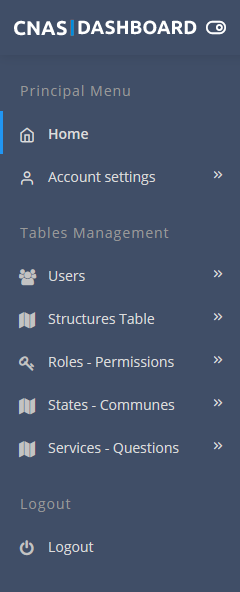
\includegraphics[width=0.2\textwidth]{SCREENSHOTS/superadmin/navbar.png}
  \caption{Superadmin Navbar}
  \label{fig:navbar}
\end{figure}
\paragraph{Comment:} The navbar provides quick access to various sections and functionalities for the superadmin.
\newpage

\begin{figure}[htbp]
    \centering
    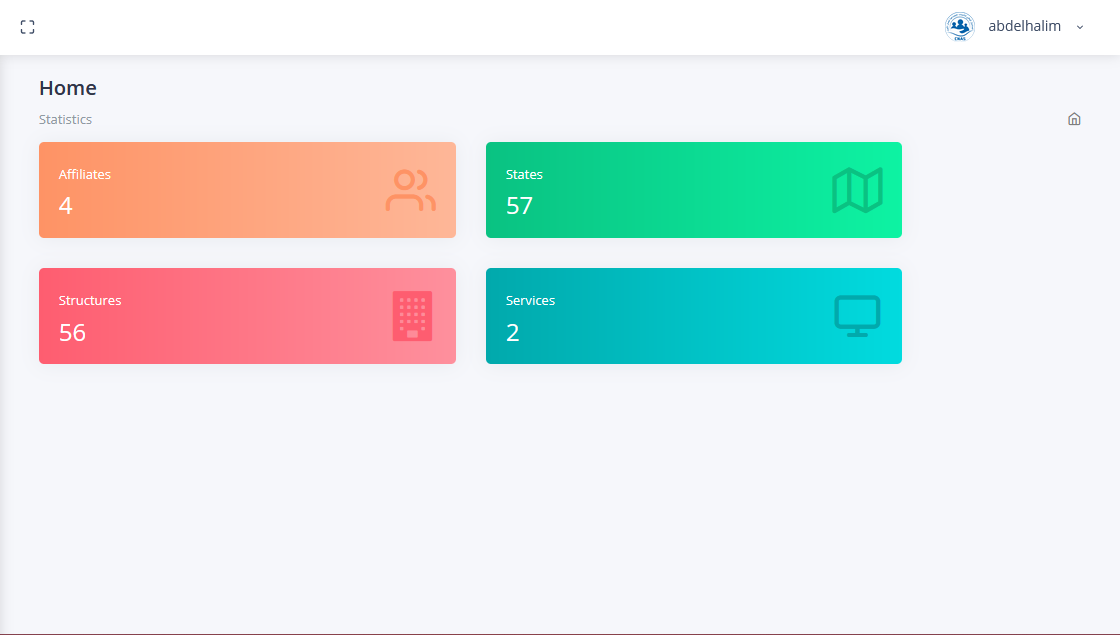
\includegraphics[width=0.7\textwidth]{SCREENSHOTS/superadmin/home.png}
    \caption{Superadmin home dashboard}
    \label{fig:home}
  \end{figure}
  \paragraph{Comment:} As shown in the screenshot above, the home page allows the superadmin to have an overall statistics on the system.


\begin{figure}[htbp]
  \centering
  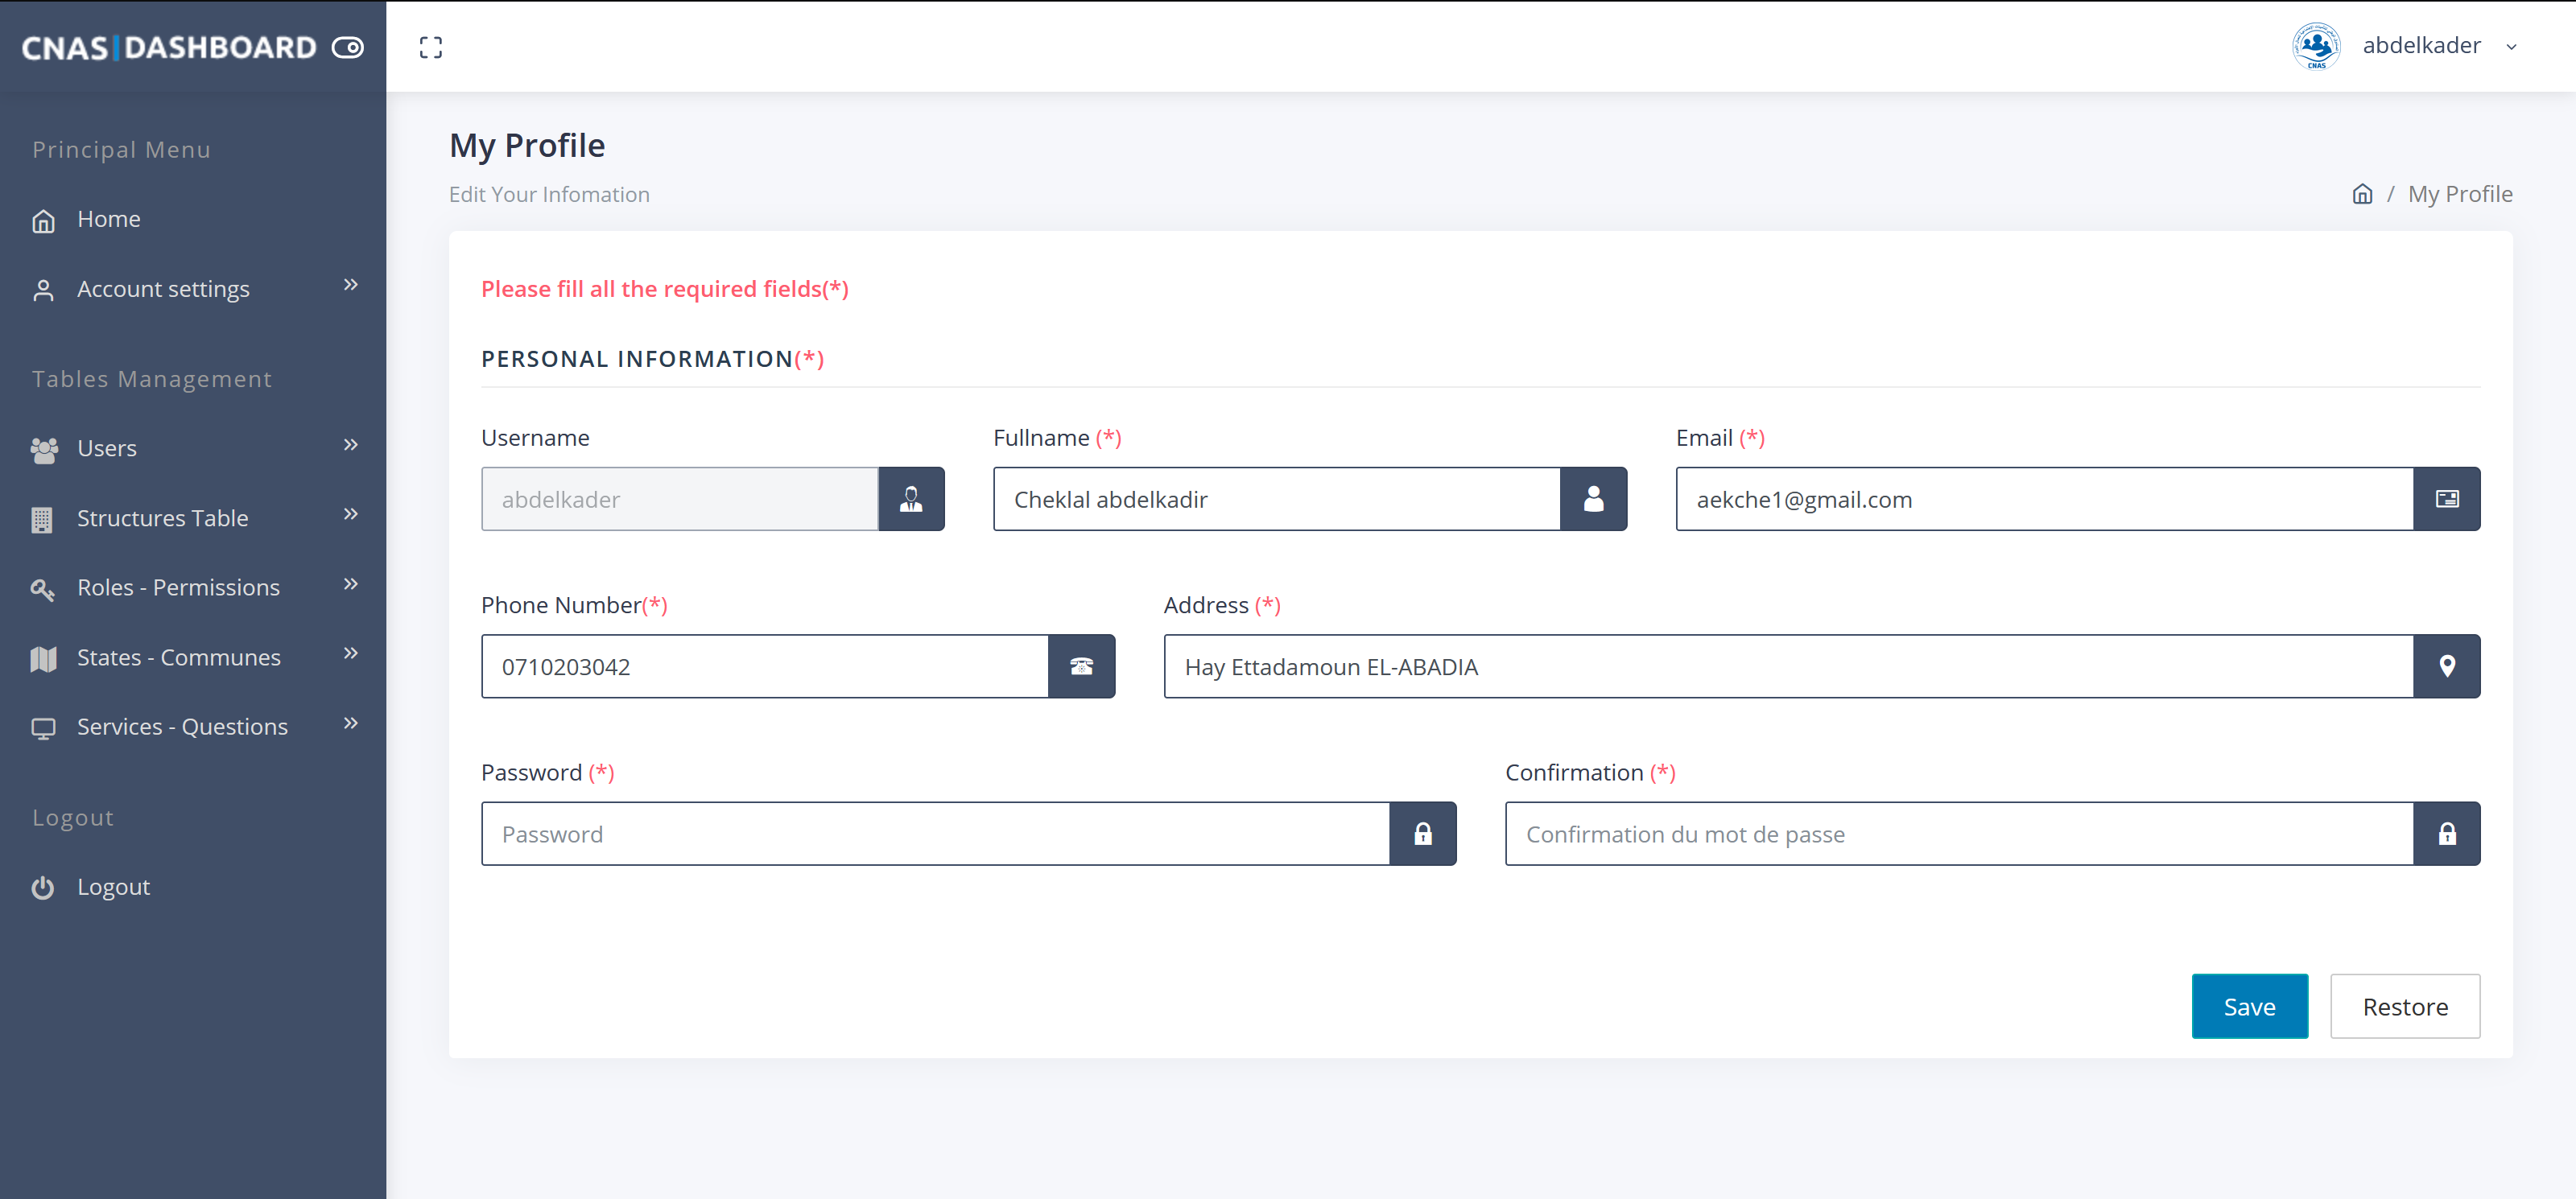
\includegraphics[width=0.7\textwidth]{SCREENSHOTS/superadmin/edit_profile.png}
  \caption{Superadmin Edit Profile}
  \label{fig:edit-profile}
\end{figure}
\paragraph{Comment:} The edit profile page allows the superadmin to modify their personal information and settings.
\newpage
% Users List
\begin{figure}[htbp]
  \centering
  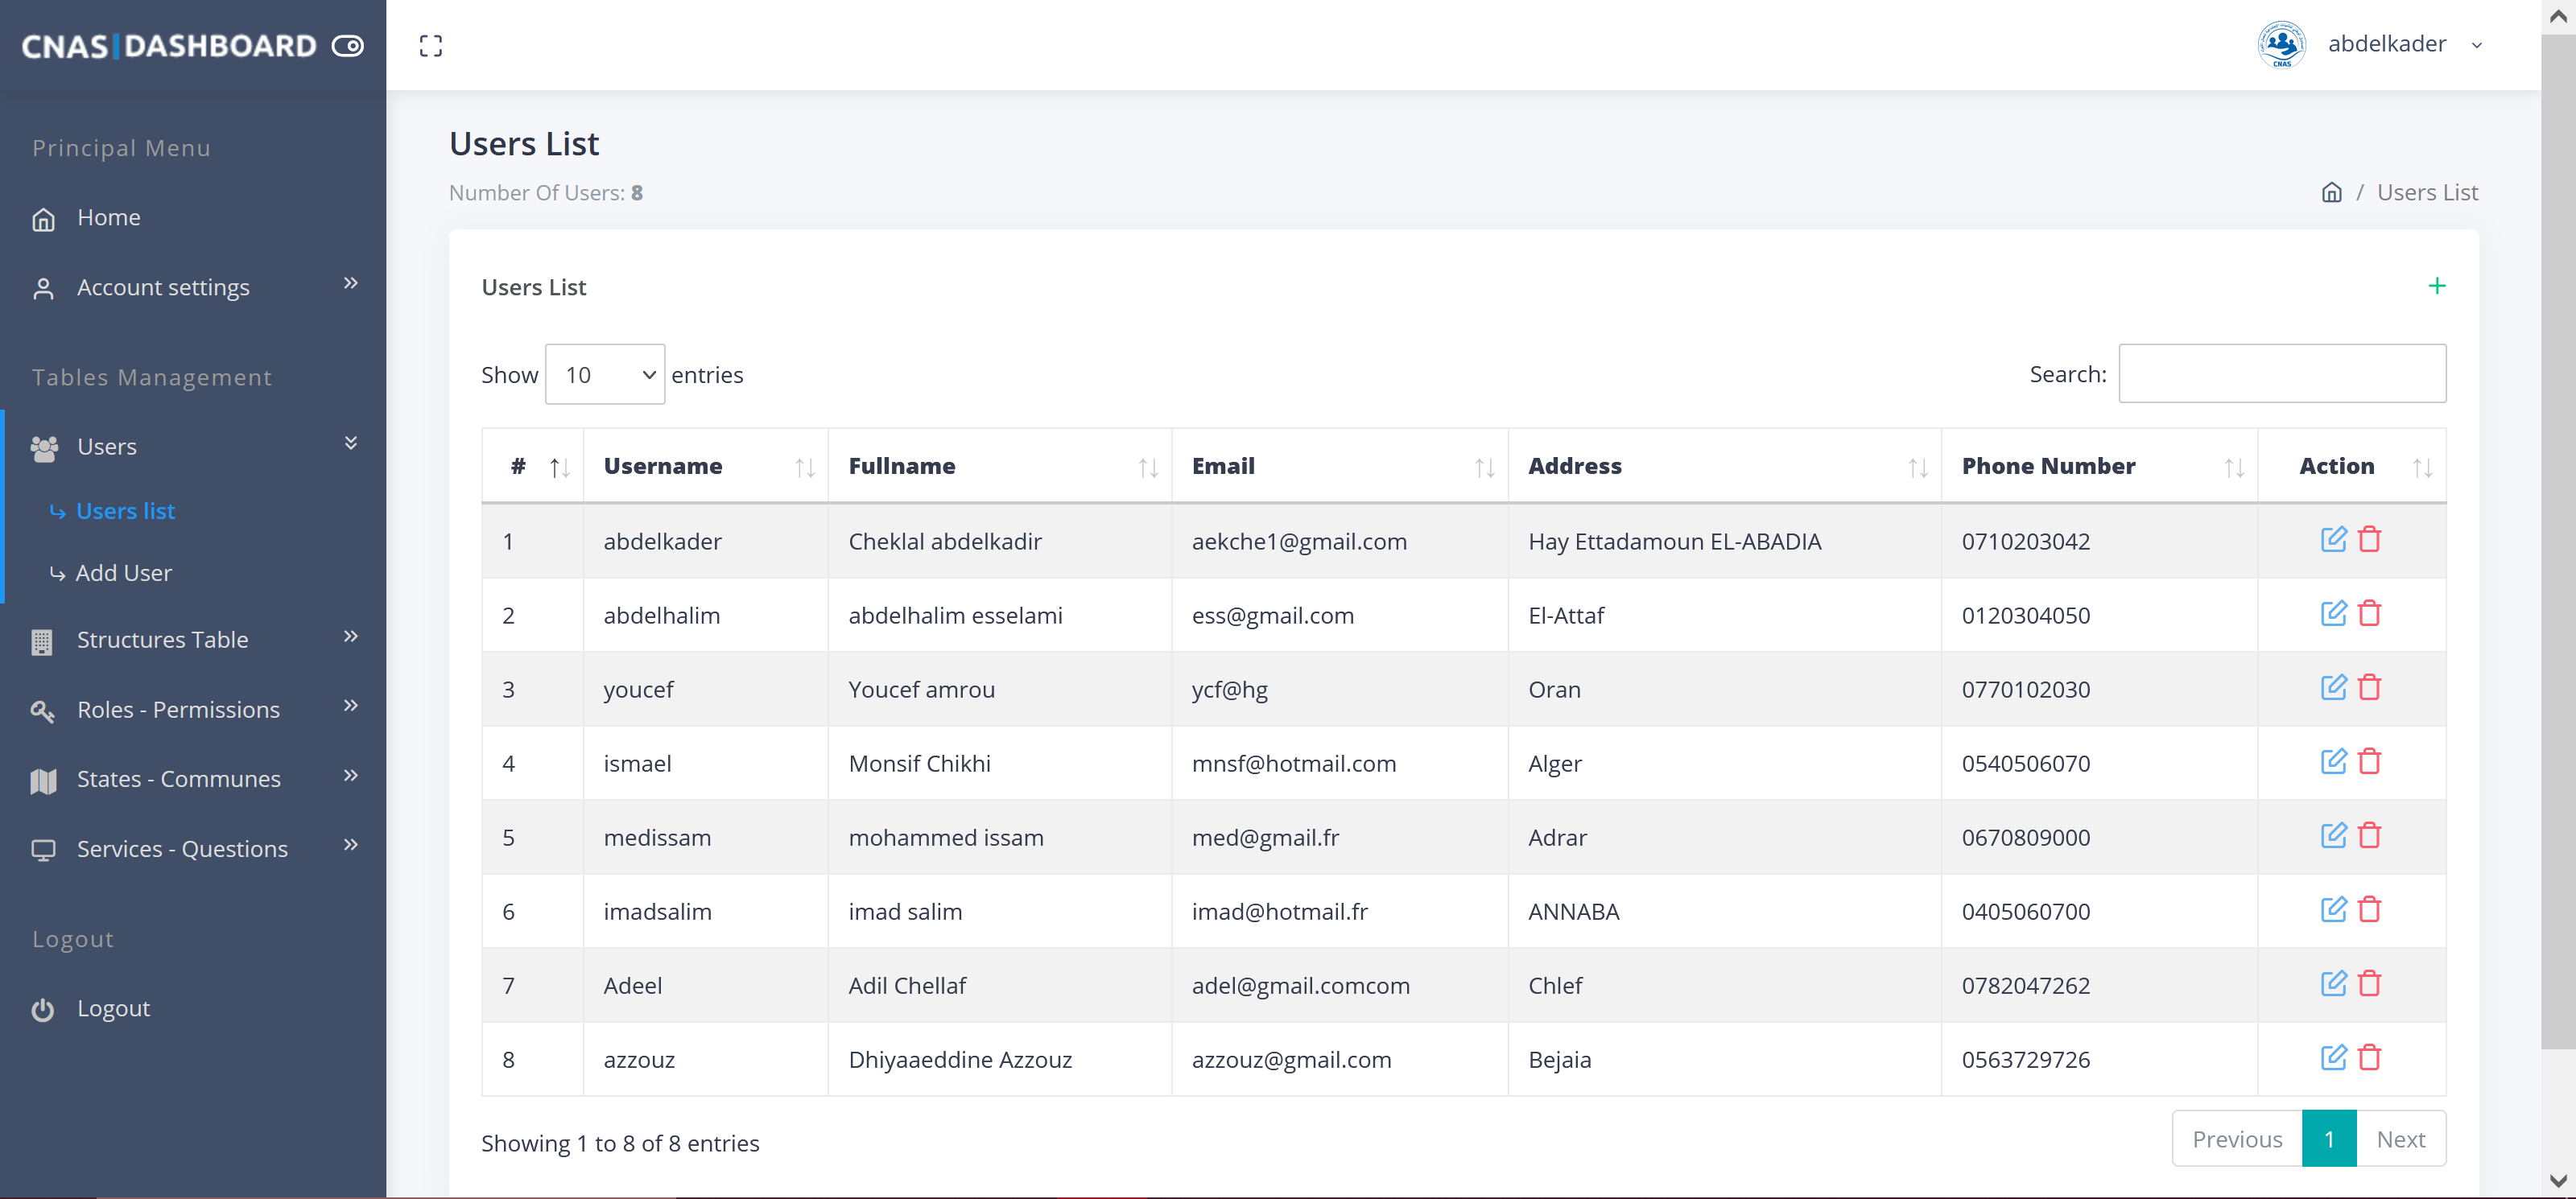
\includegraphics[width=0.7\textwidth]{SCREENSHOTS/superadmin/users_list.png}
  \caption{Superadmin Users List}
  \label{fig:users-list}
\end{figure}
\paragraph{Comment:} The users list provides an overview of all registered users, allowing the superadmin to manage user accounts, roles, and permissions.

\begin{figure}[htbp]
    \centering
    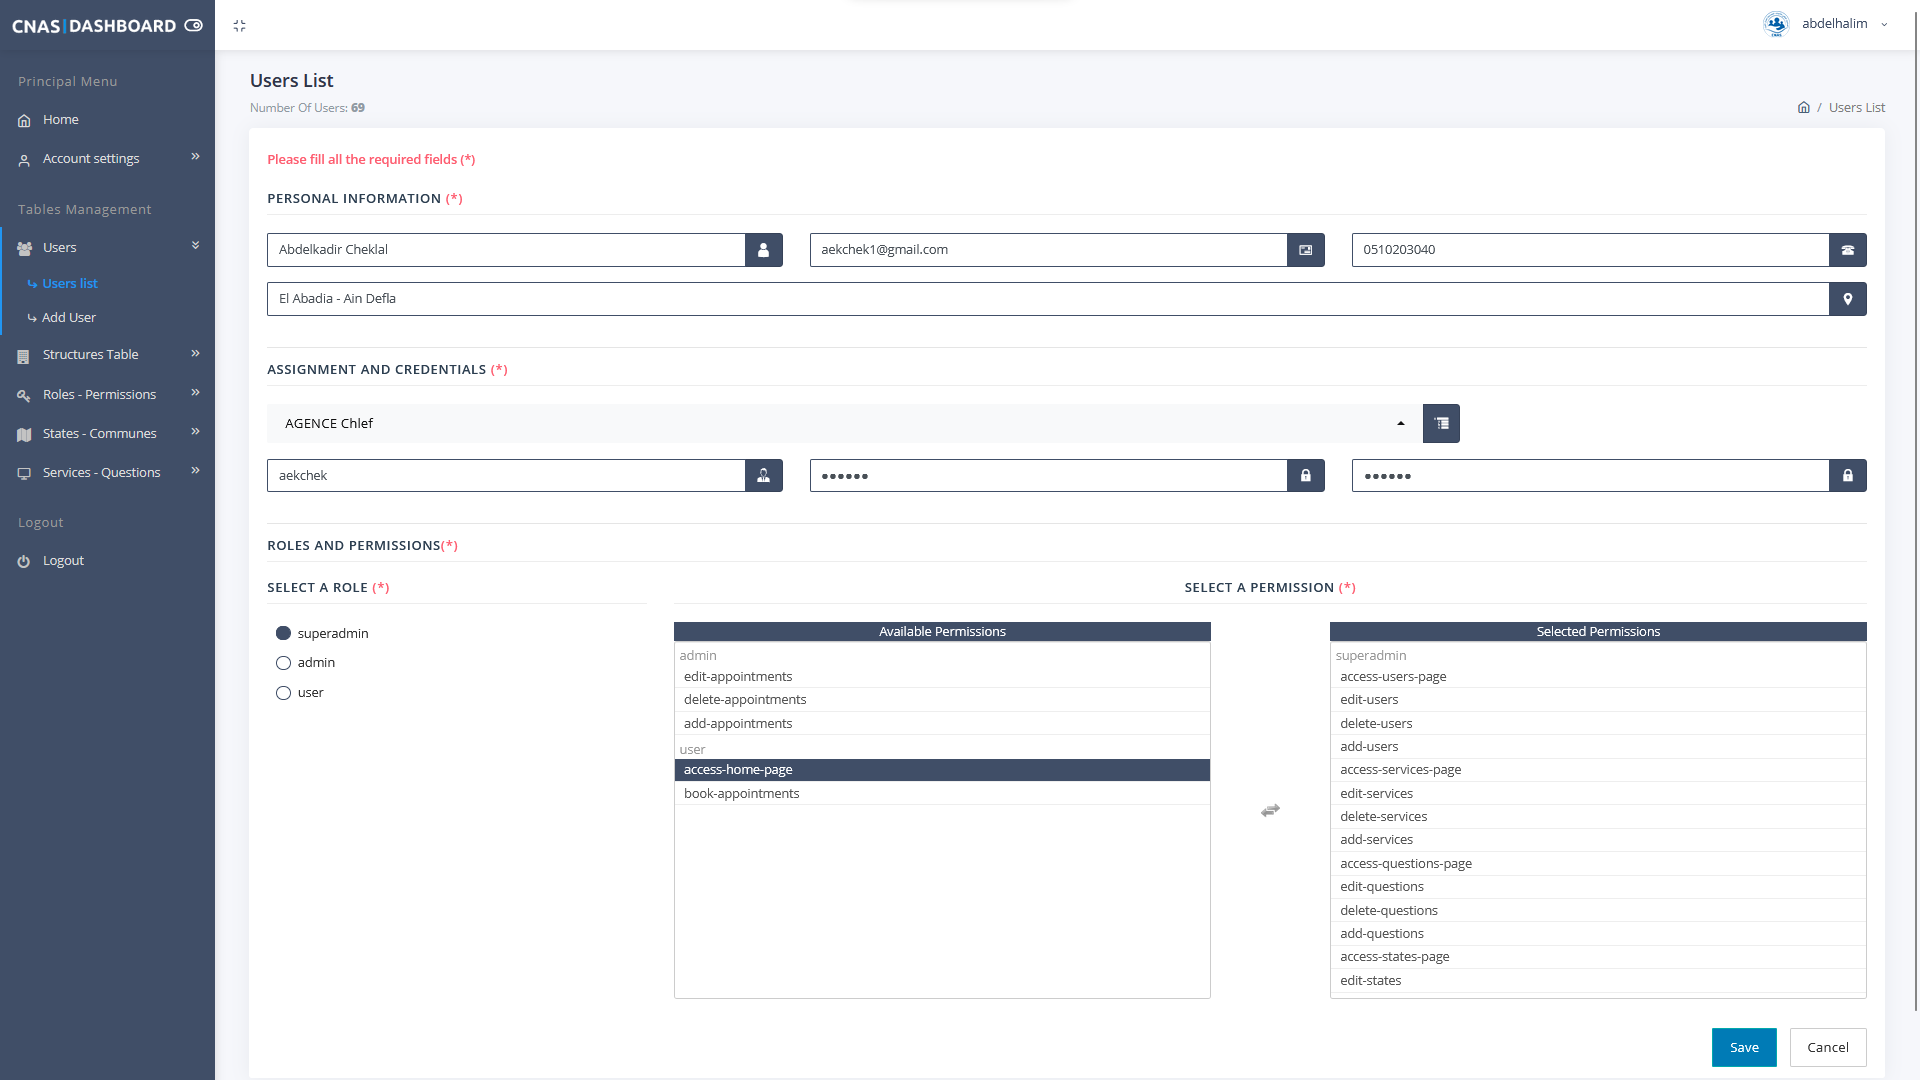
\includegraphics[width=0.7\textwidth]{SCREENSHOTS/superadmin/edit_user.png}
    \caption{Superadmin Edit User}
    \label{fig:edit-user}
  \end{figure}
  \paragraph{Comment:} The screenshot above shows the "Edit User" screen of the application. This screen allows the superadmin to modify user details such as fullname, email, , password, role, and permissions. The form fields are clearly labeled, and the user's current information is pre-populated for easy editing. The "Save" button can be used to save the changes made to the user's profile.
\newpage 
% Add User
\begin{figure}[htbp]
  \centering
  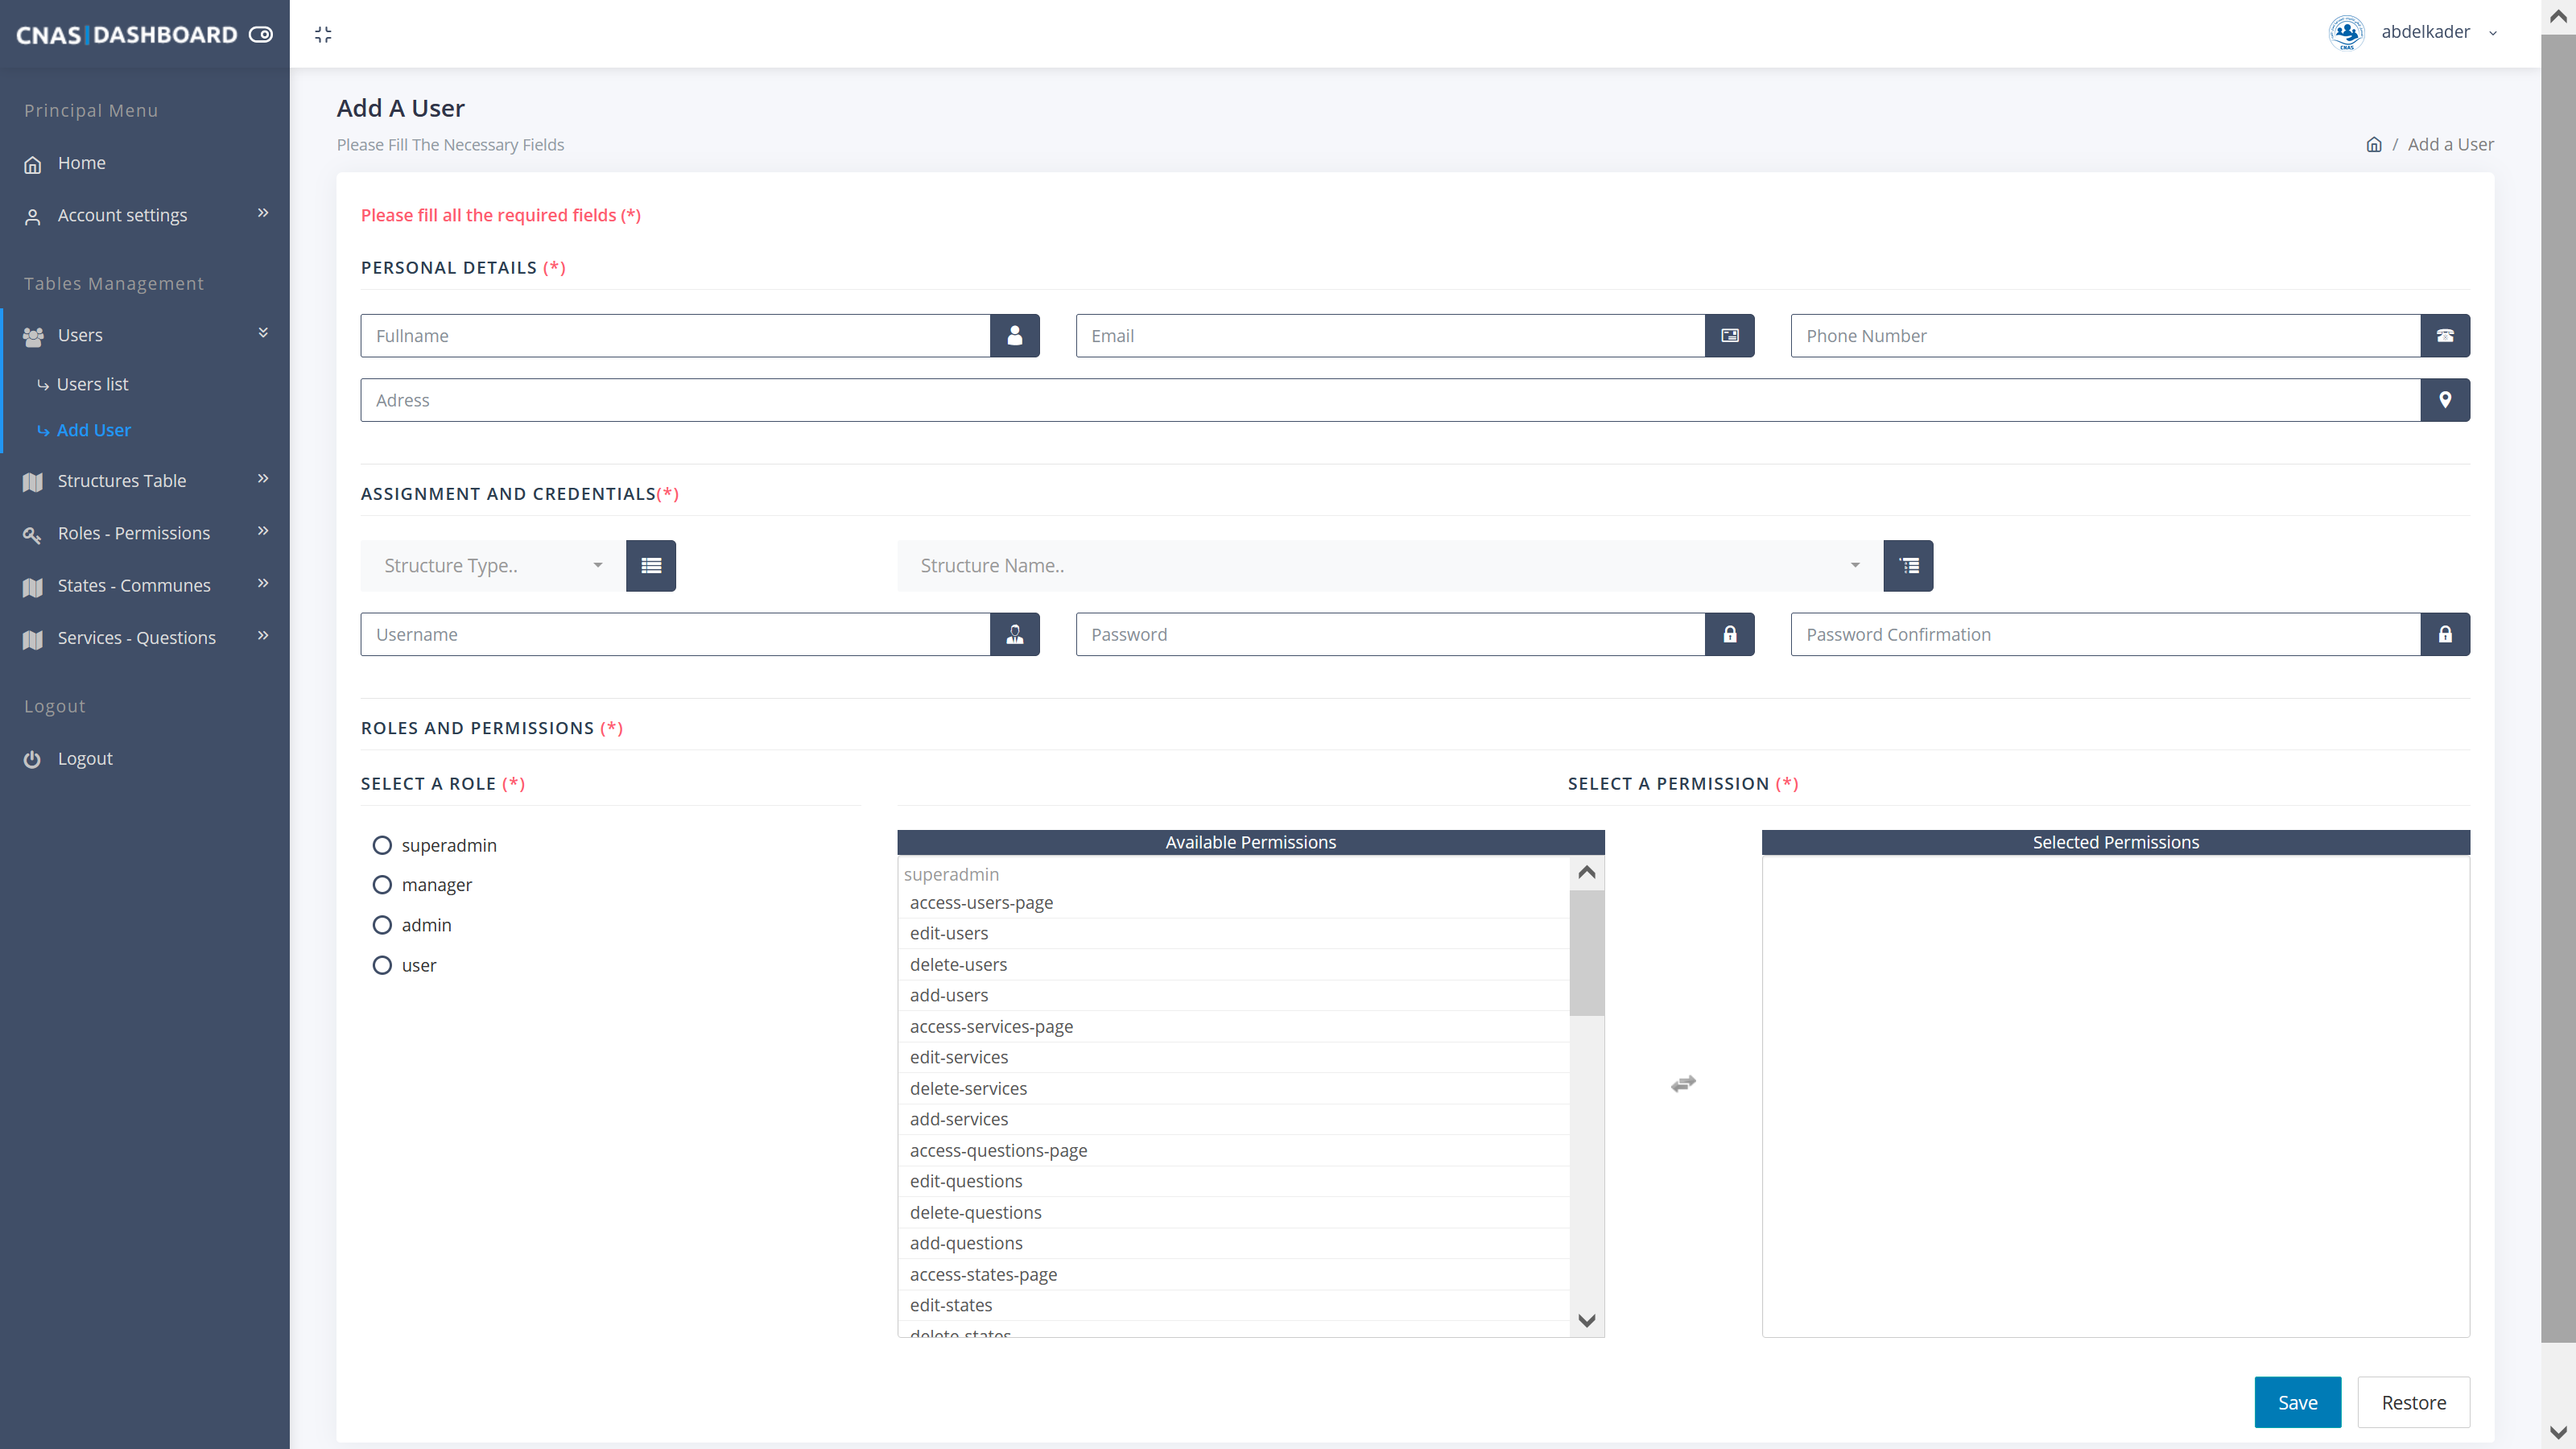
\includegraphics[width=0.7\textwidth]{SCREENSHOTS/superadmin/add_user.png}
  \caption{Superadmin Add User}
  \label{fig:add-user}
\end{figure}
\paragraph{Comment:} The add user page allows the superadmin to create a new user account by specifying relevant details and assigning appropriate roles and permissions.

% Structure List
\begin{figure}[htbp]
  \centering
  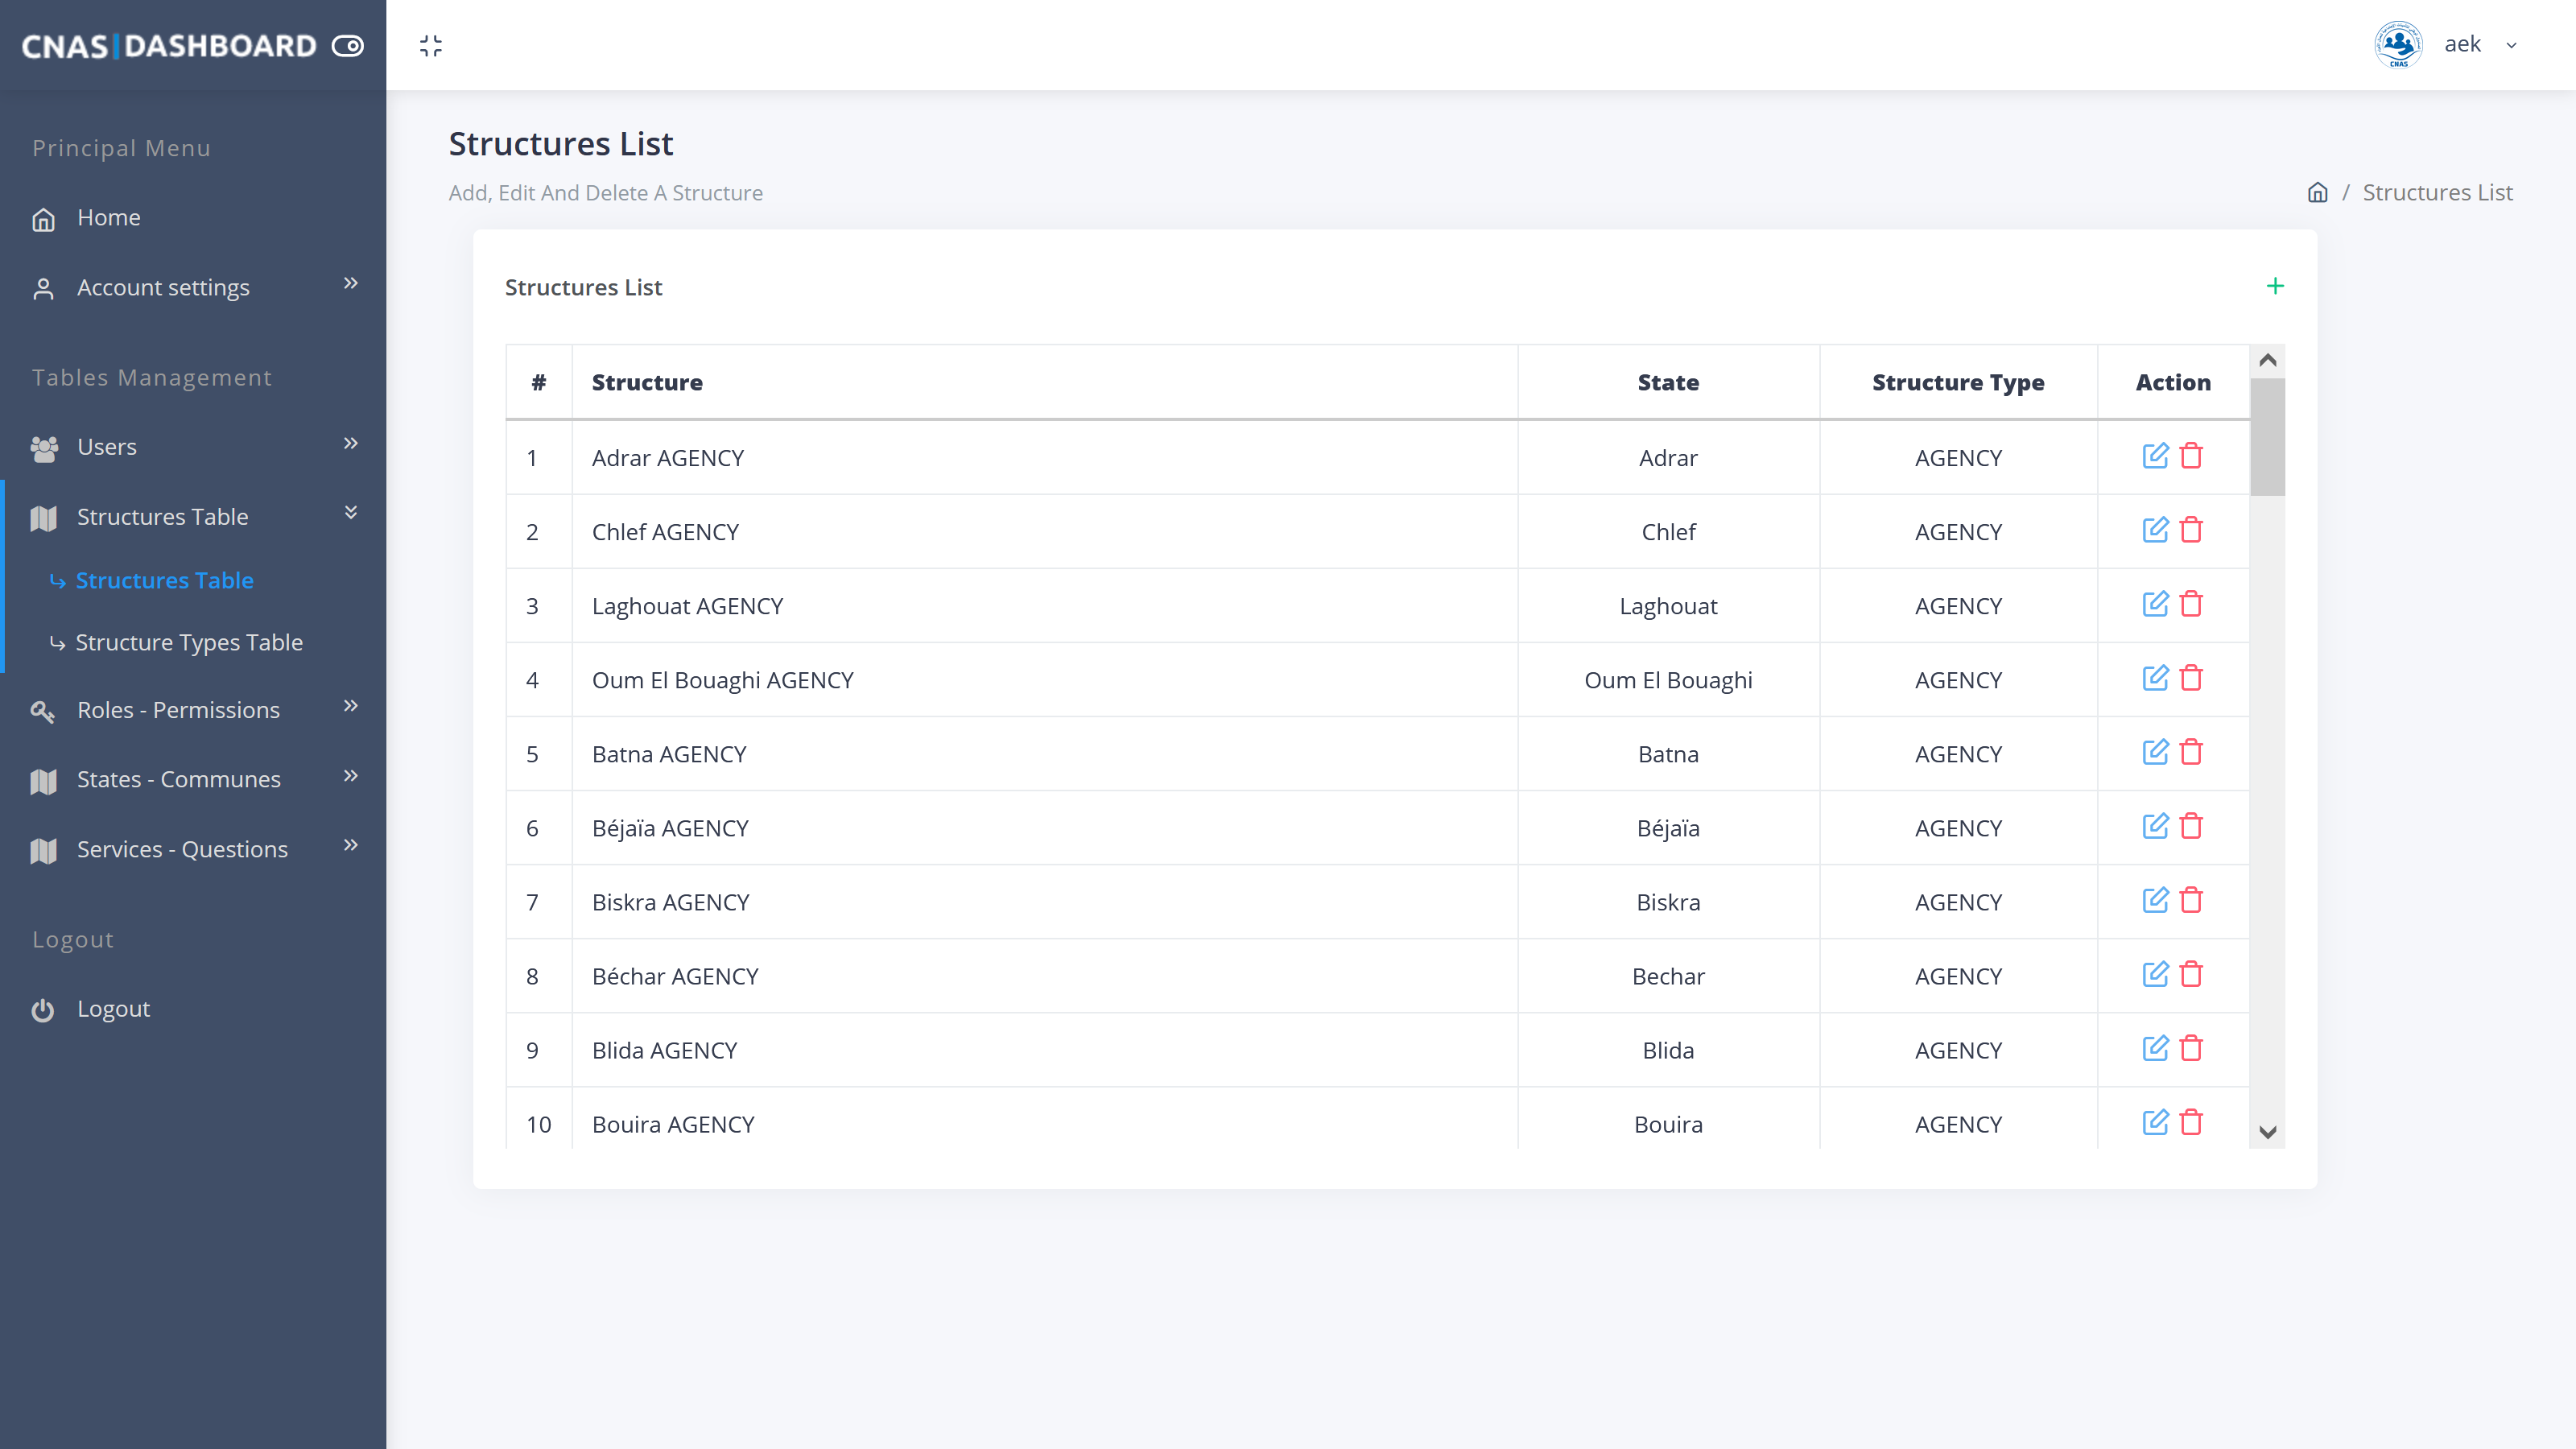
\includegraphics[width=0.7\textwidth]{SCREENSHOTS/superadmin/structures_list.png}
  \caption{Superadmin Structures List}
  \label{fig:structures-list}
\end{figure}
\paragraph{Comment:} The structures list displays all registered structures along with their details and options for management.
\newpage 

% Structure Types List
\begin{figure}[htbp]
  \centering
  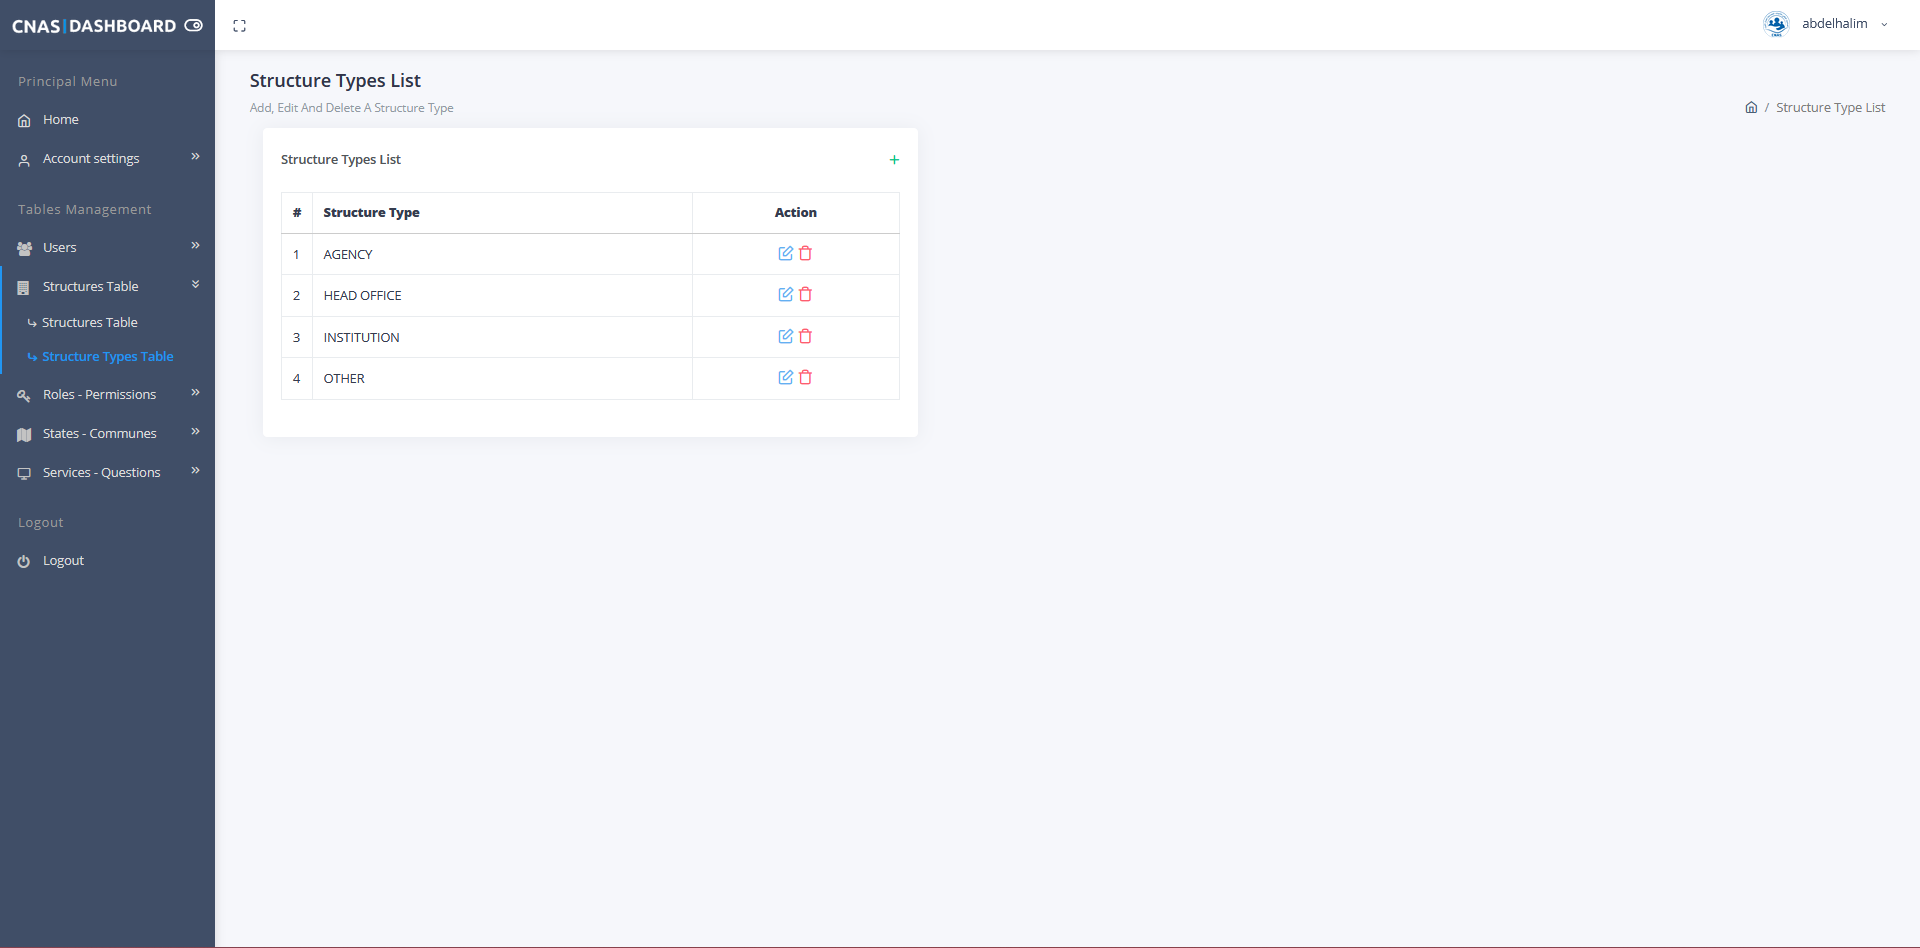
\includegraphics[width=0.7\textwidth]{SCREENSHOTS/superadmin/structureTypes_list.png}
  \caption{Superadmin Structure Types List}
  \label{fig:structure-types-list}
\end{figure}
\paragraph{Comment:} The structure types list shows different types of structures available in the system and allows the superadmin to manage them.

% Roles List
\begin{figure}[htbp]
  \centering
  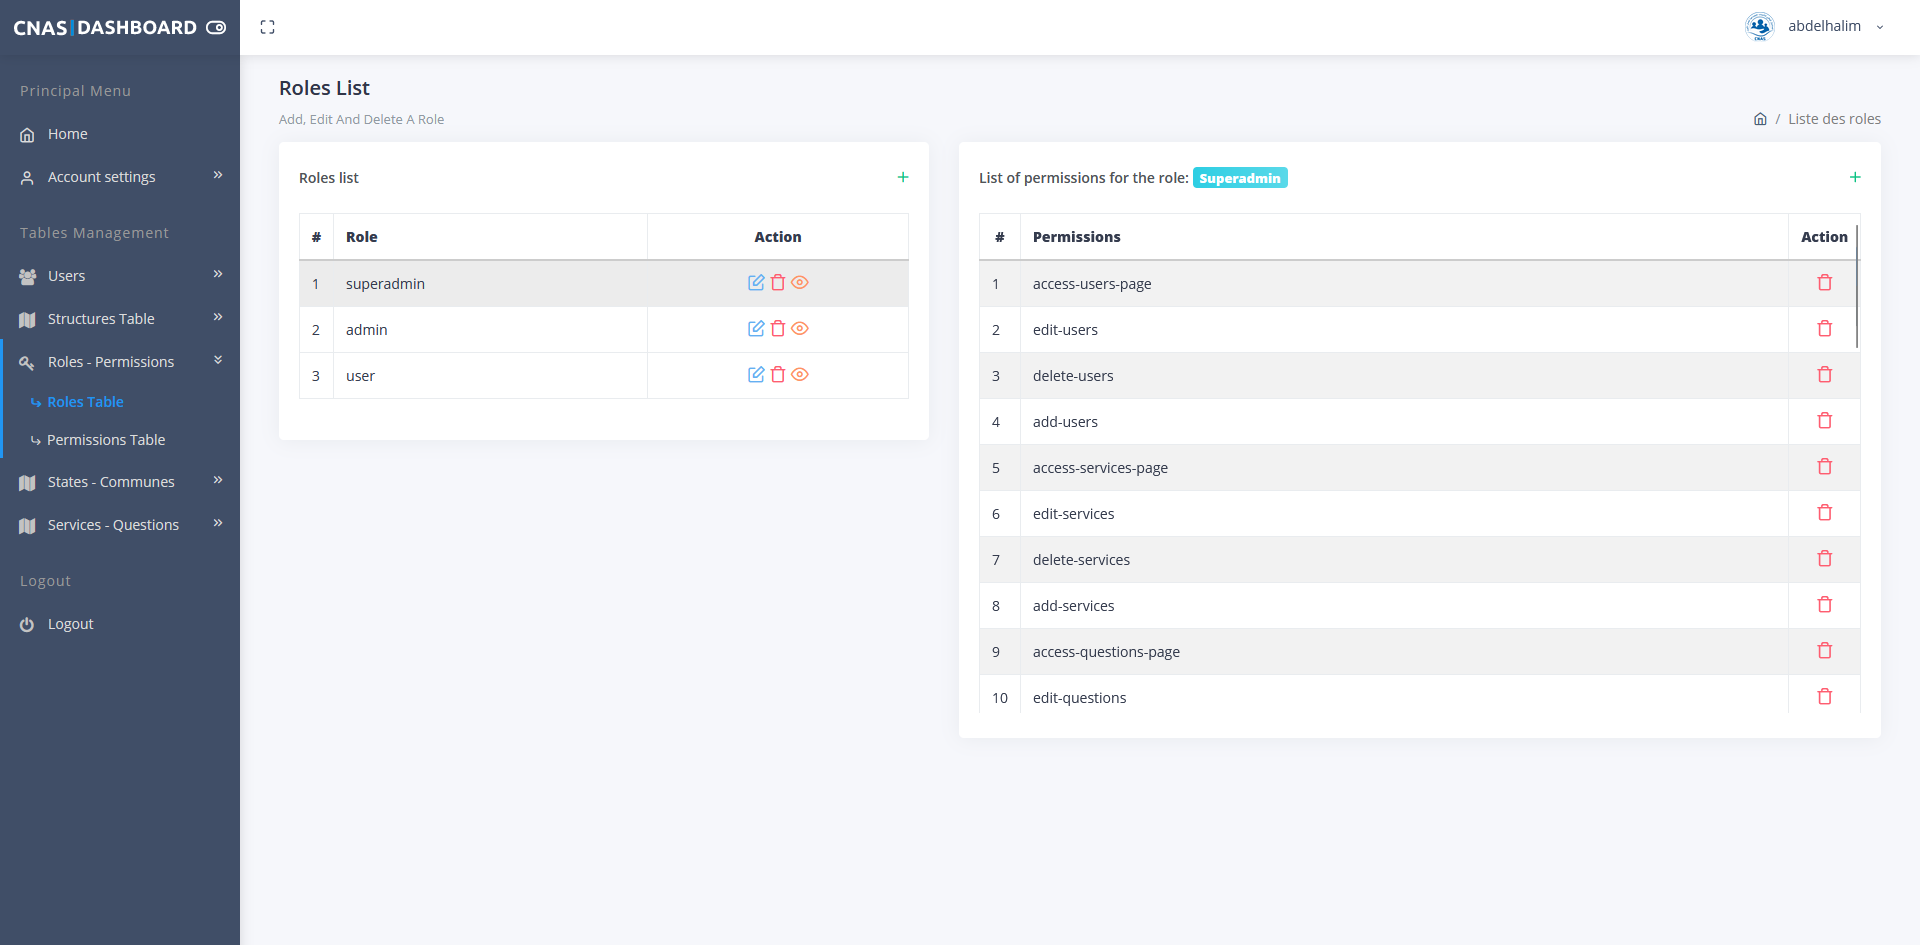
\includegraphics[width=0.7\textwidth]{SCREENSHOTS/superadmin/roles_list.png}
  \caption{Superadmin Roles List}
  \label{fig:roles-list}
\end{figure}
\paragraph{Comment:} The roles list displays all available user roles and their associated permissions, providing the superadmin with role management capabilities.
\newpage



% Permissions List
\begin{figure}[htbp]
    \centering
    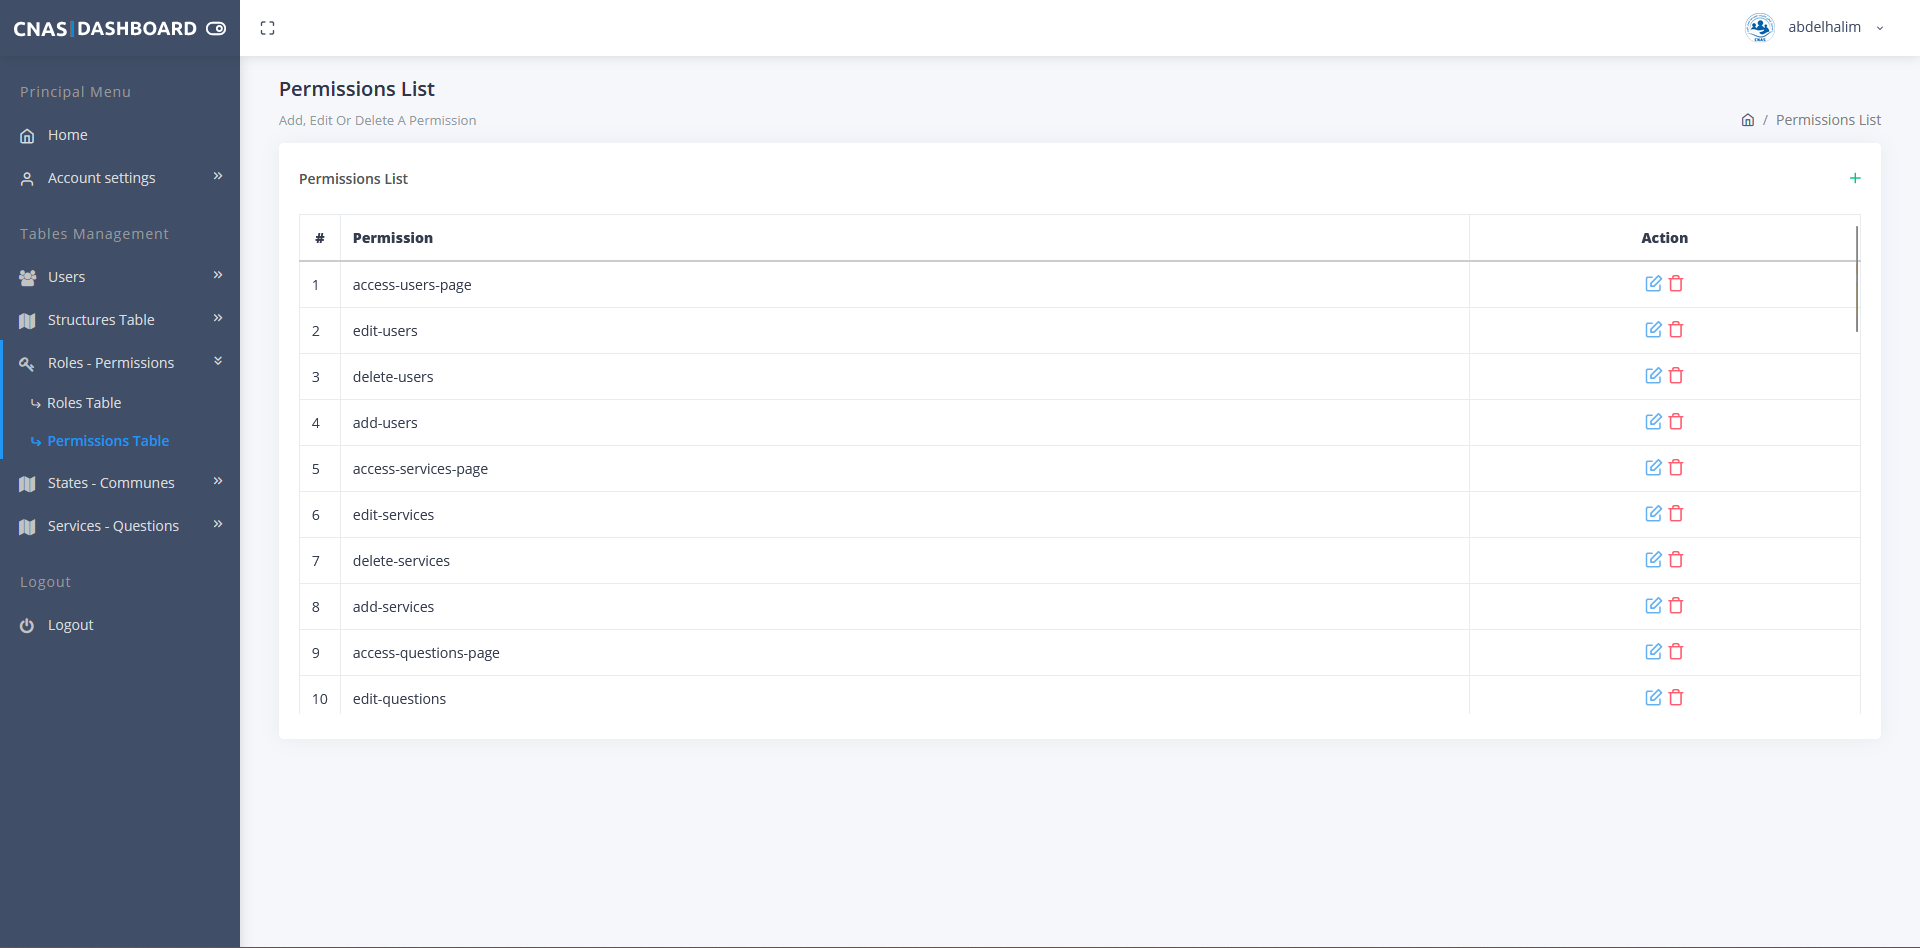
\includegraphics[width=0.7\textwidth]{SCREENSHOTS/superadmin/permissions_list.png}
    \caption{Superadmin Permissions List}
    \label{fig:permissions-list}
  \end{figure}
  \paragraph{Comment:} The screenshot above displays the list of permissions available in the system. These permissions determine the actions and functionalities that can be accessed by different user roles.

  % States List
  \begin{figure}[htbp]
    \centering
    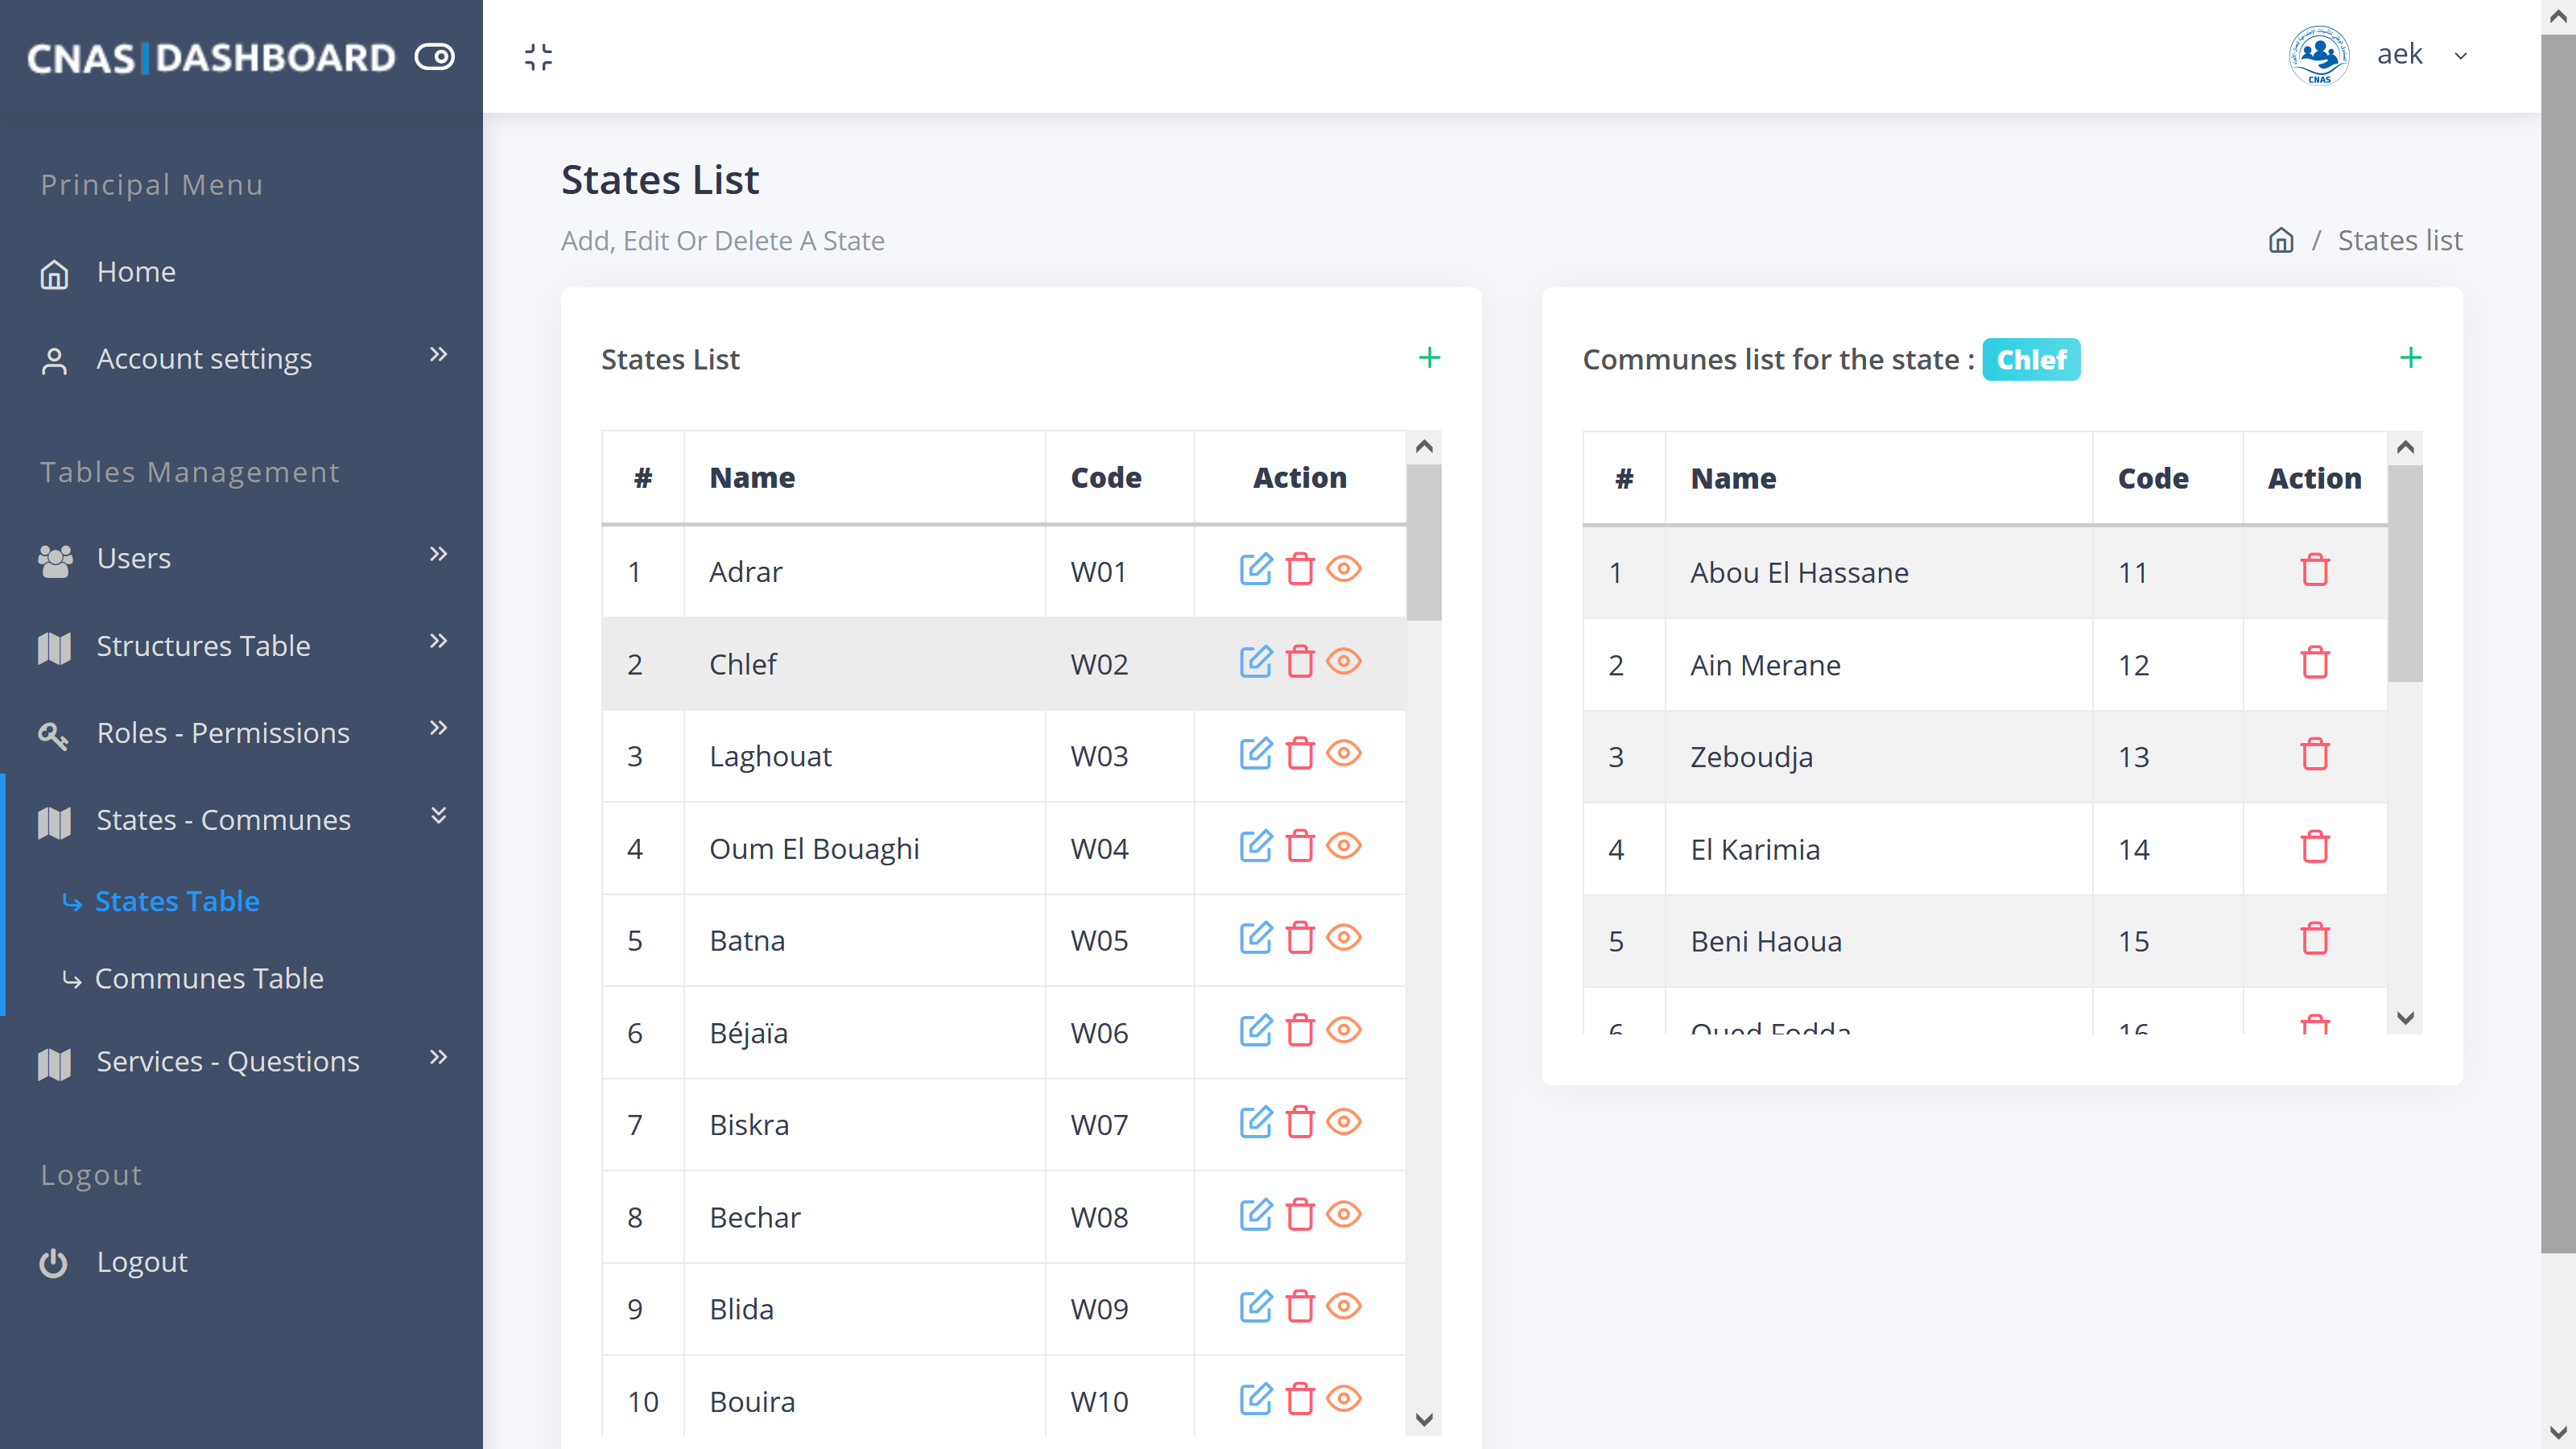
\includegraphics[width=0.7\textwidth]{SCREENSHOTS/superadmin/states_communes.png}
    \caption{Superadmin States List}
    \label{fig:states-list}
\end{figure}
\paragraph{Comment:} The states list displays all available states and their relevant information, enabling the superadmin to manage state-related data.
\newpage

% Communes List
\begin{figure}[htbp]
    \centering
    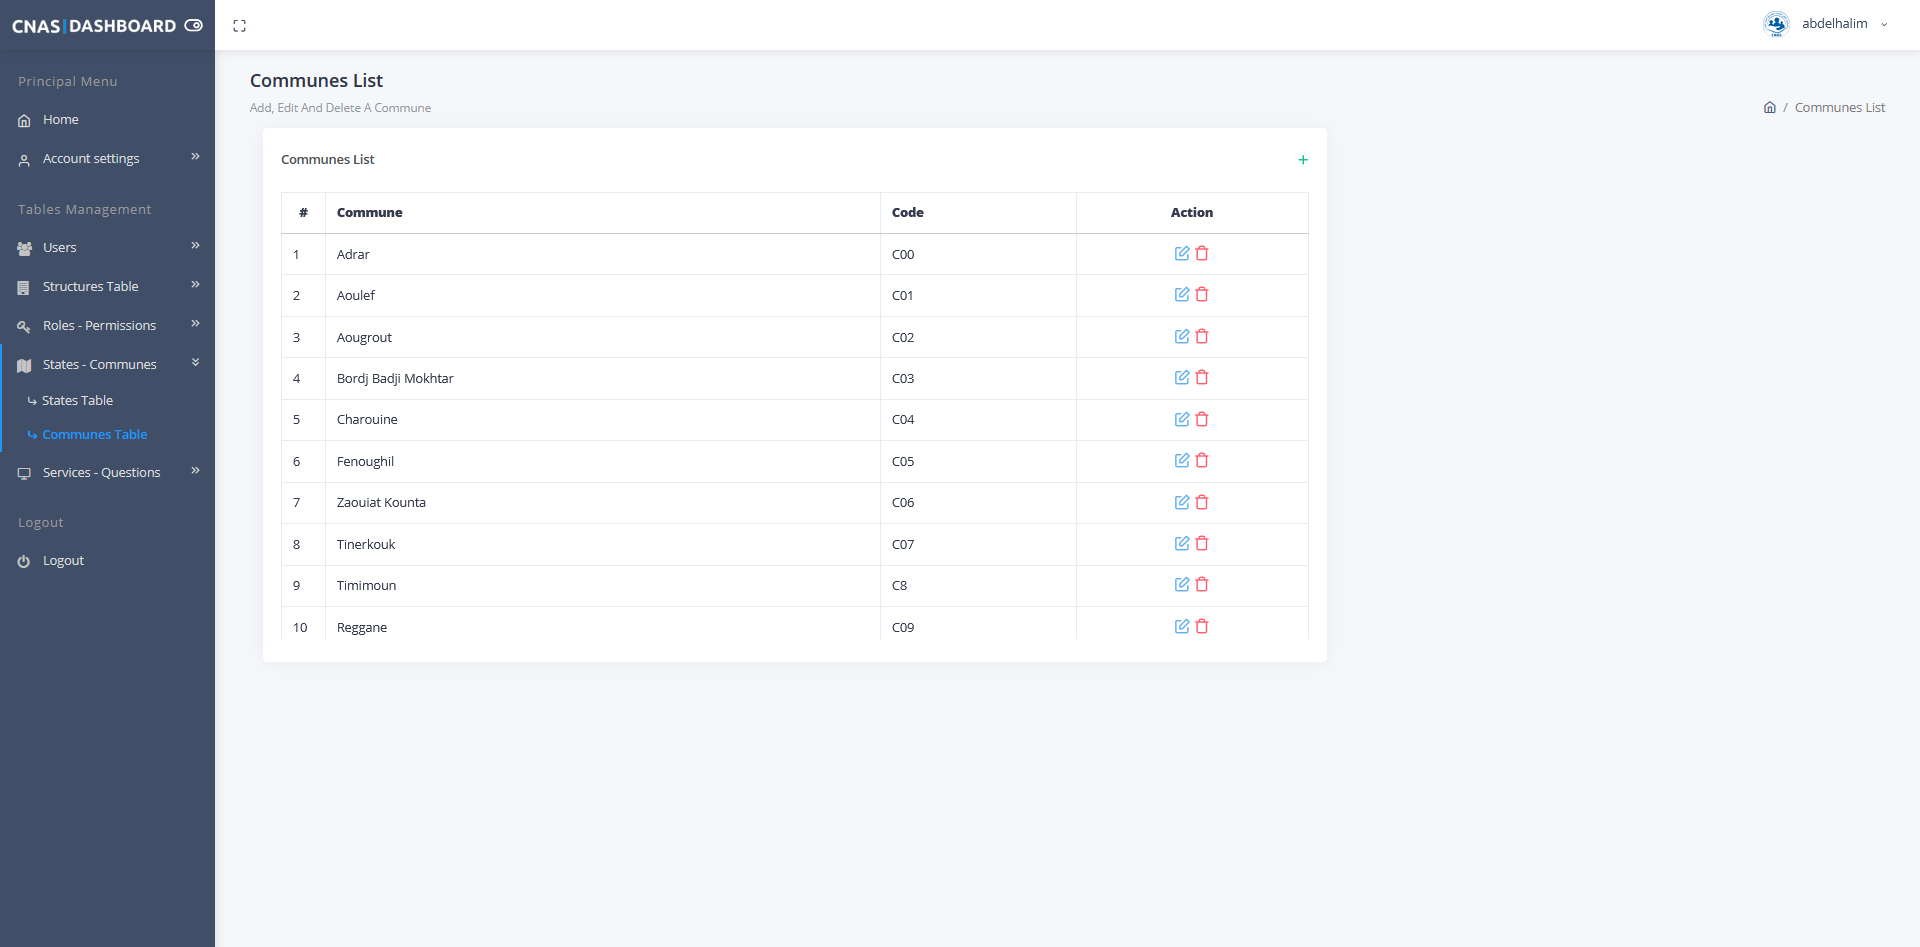
\includegraphics[width=0.7\textwidth]{SCREENSHOTS/superadmin/communes.png}
  \caption{Superadmin Communes List}
  \label{fig:communes-list}
\end{figure}
\paragraph{Comment:} The communes list showcases all available communes and their relevant details, allowing the superadmin to manage commune-related data.

\begin{figure}[htbp]
    \centering
    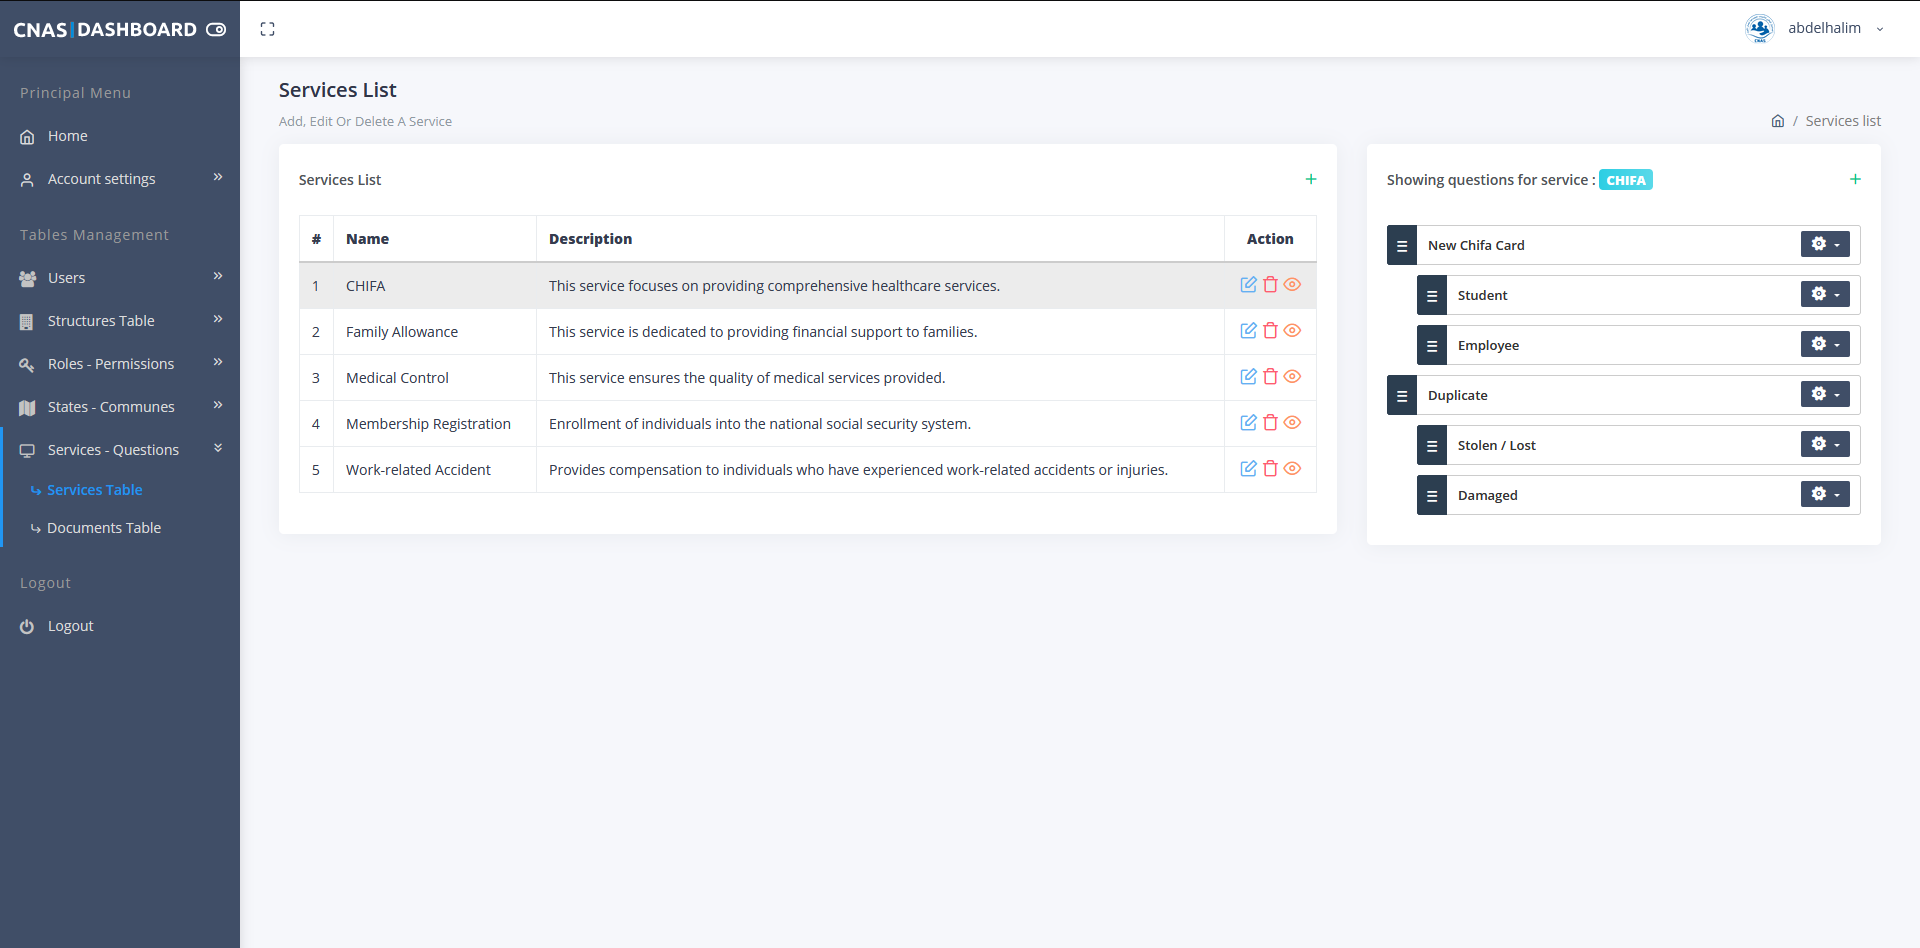
\includegraphics[width=0.7\textwidth]{SCREENSHOTS/superadmin/services_questions.png}
    \caption{Superadmin Services - Questions List}
    \label{fig:services-list}
\end{figure}
\paragraph{Comment:} The screenshot above displays the Services Questions List, which allows users to view and manage the questions related to various services. It provides an organized interface where superadmin can add, edit, or delete questions to gather necessary information from users. This feature enables efficient data collection and improves the overall user experience.
\newpage
\begin{figure}[htbp]
    \centering
    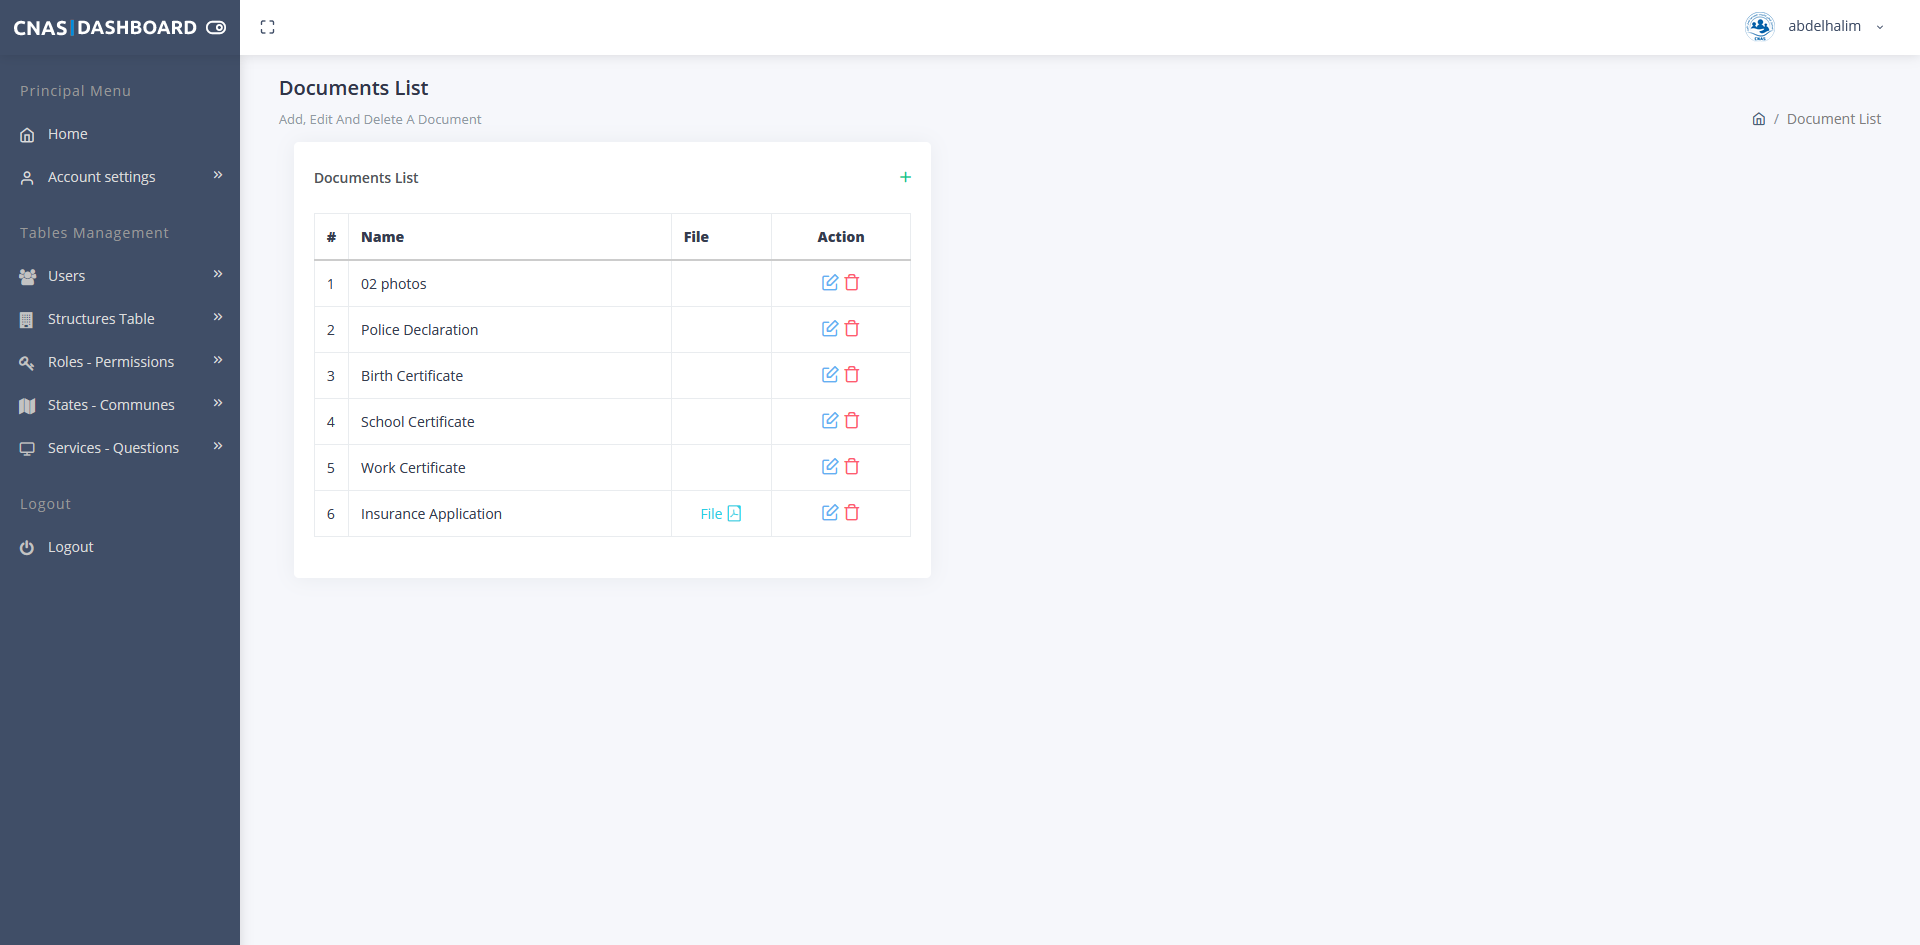
\includegraphics[width=0.7\textwidth]{SCREENSHOTS/superadmin/documents_list.png}
    \caption{Superadmin Documents List}
    \label{fig:documents-list}
\end{figure}
\paragraph{Comment:} The screenshot above showcases the Documents List, which provides superadmin with a centralized repository for managing and organizing important documents.

\rule{\linewidth}{1pt}

\vspace{1cm}

\item \textbf{Admin:}

  \begin{figure}[htbp]
    \centering
    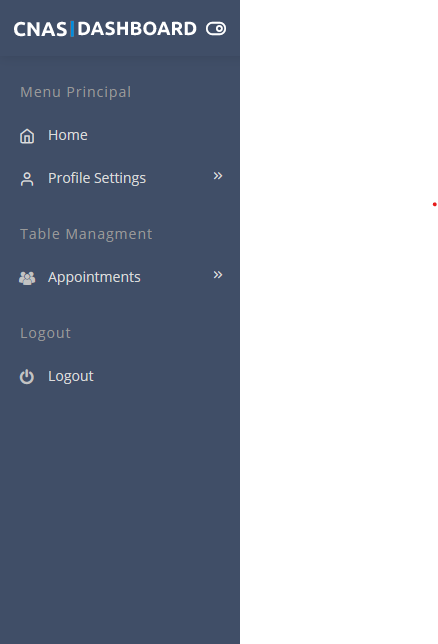
\includegraphics[width=0.3\textwidth]{SCREENSHOTS/admin/navbar.png}
    \caption{Admin Navbar}
    \label{fig:admin-navbar}
\end{figure}
\paragraph{Comment:} The screenshot above displays the navigation bar for the admin panel. It provides easy access to various administrative functionalities and sections of the application.

\begin{figure}[htbp]
  \centering
  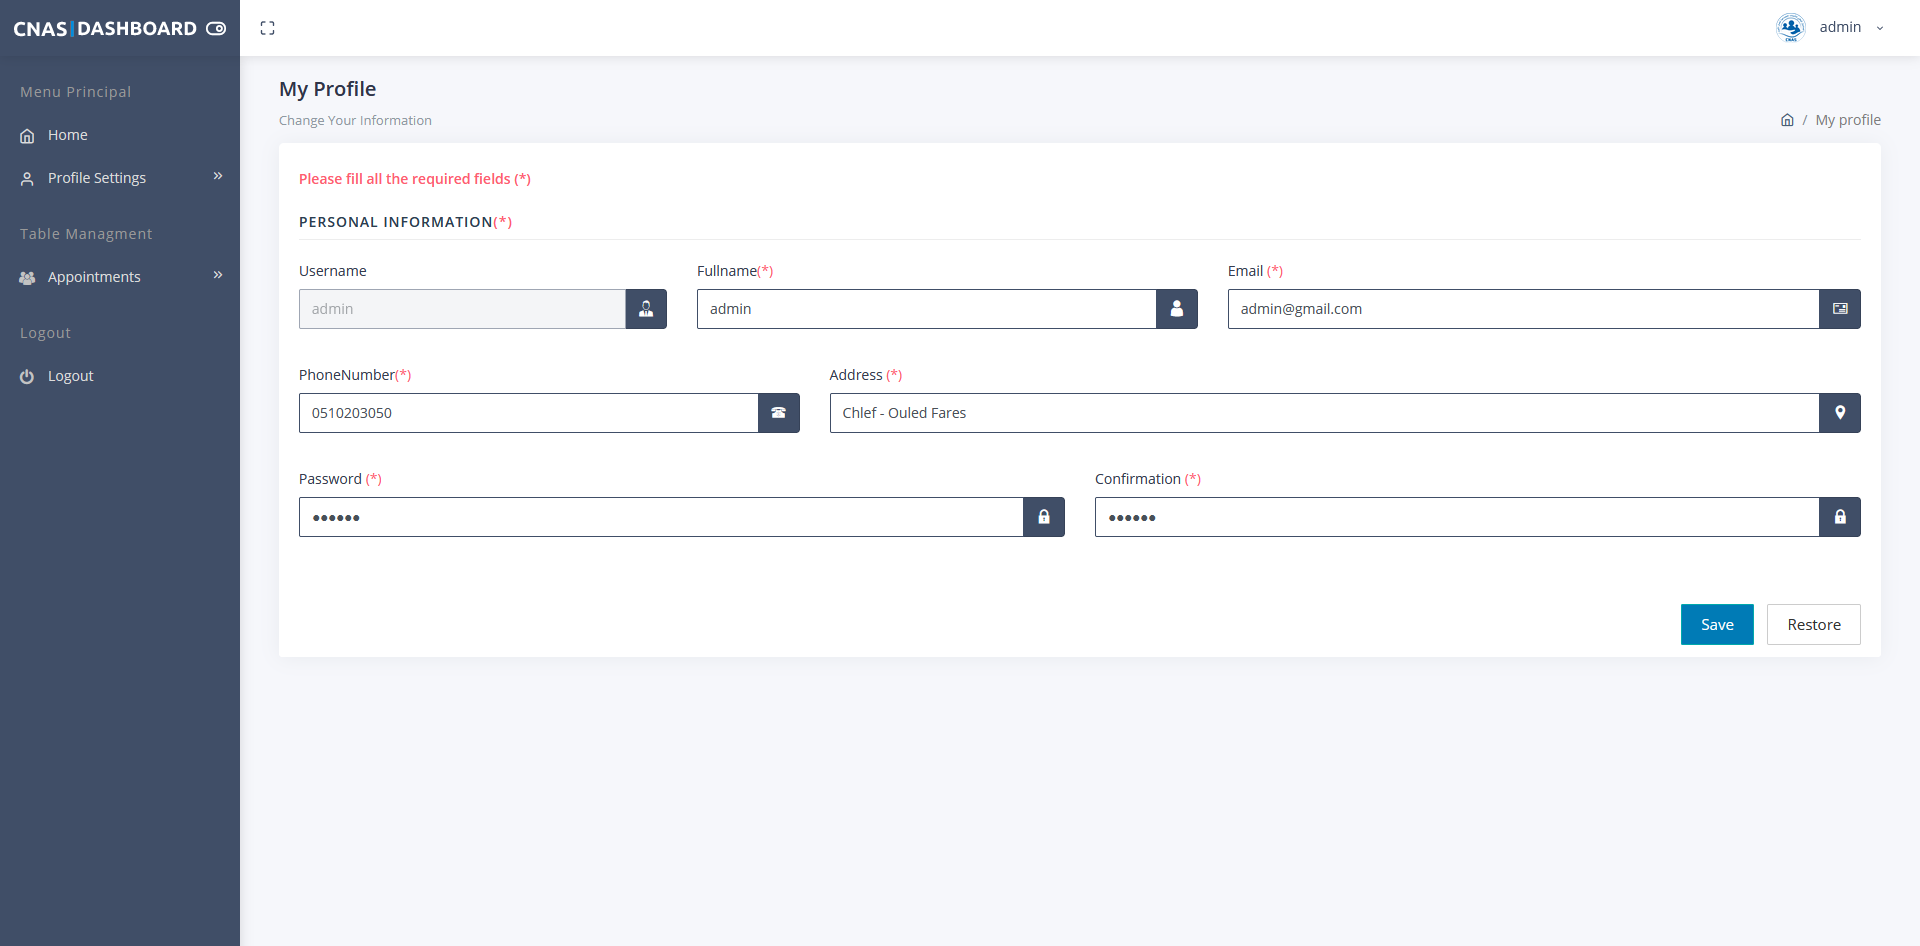
\includegraphics[width=0.7\textwidth]{SCREENSHOTS/admin/edit_profile.png}
  \caption{Admin Edit Profile}
  \label{fig:admin-edit-profile}
\end{figure}
\paragraph{Comment:} The edit profile page allows the admin to modify their personal information and settings.


\begin{figure}[htbp]
    \centering
    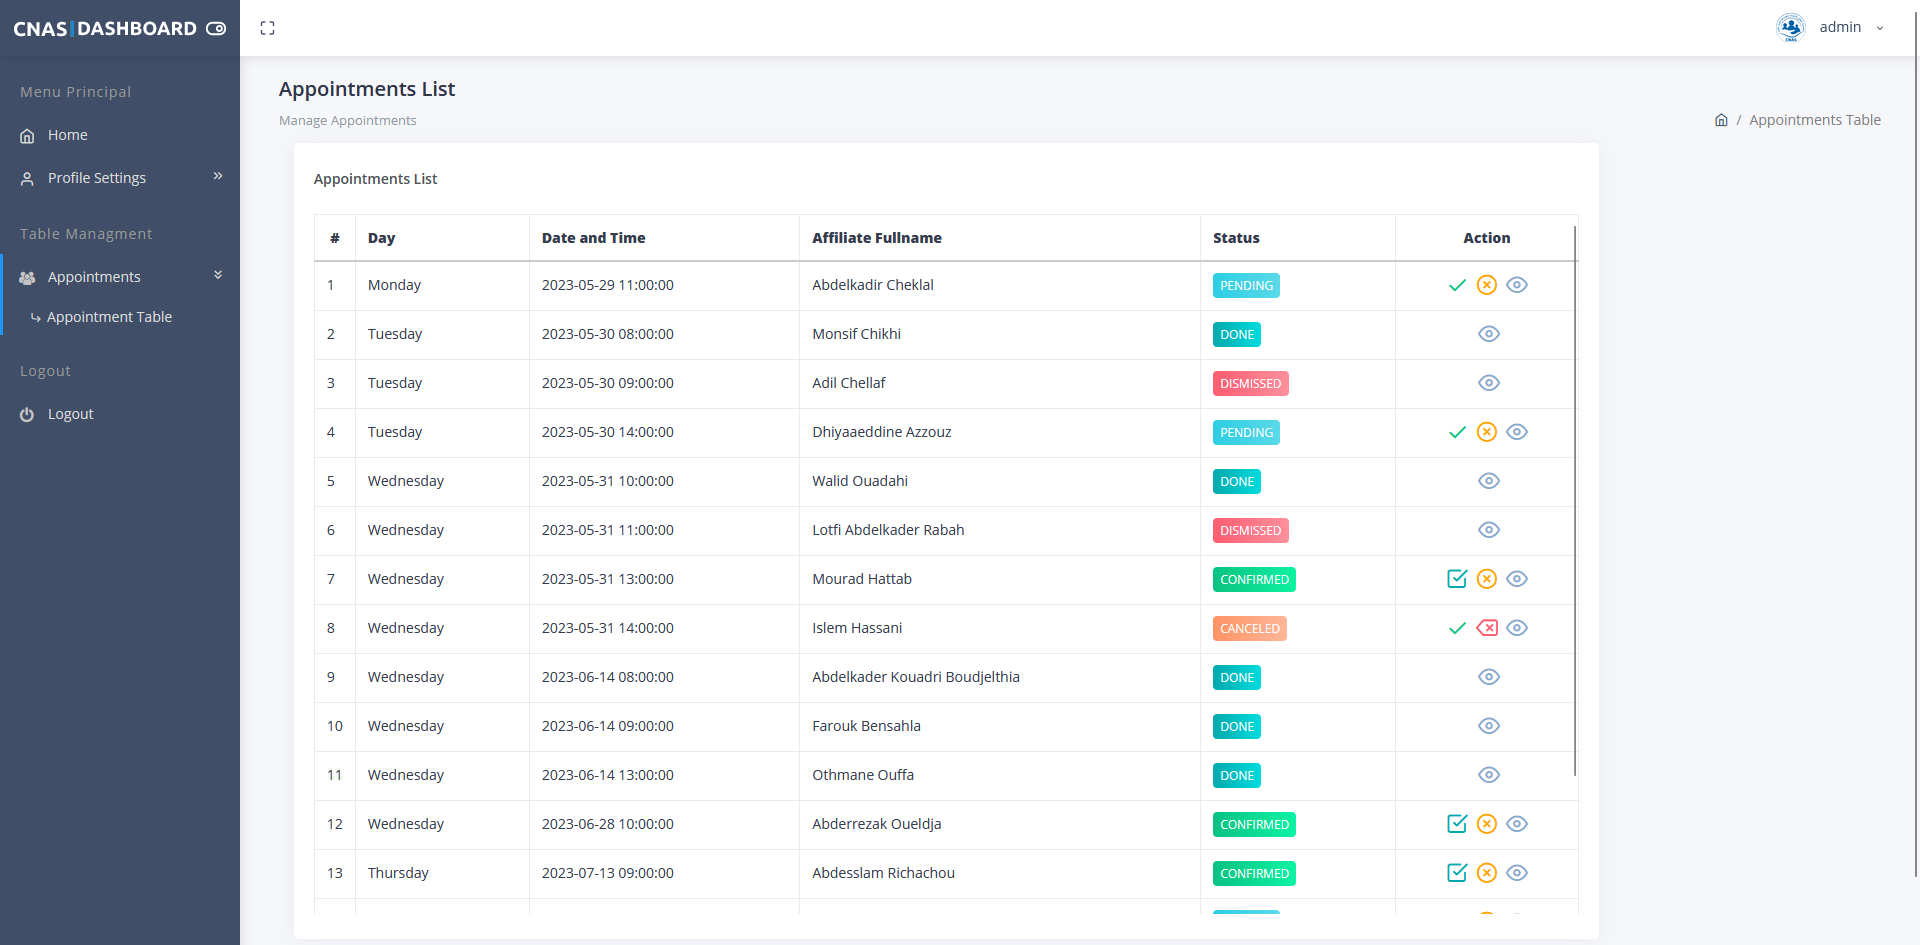
\includegraphics[width=0.7\textwidth]{SCREENSHOTS/admin/appointments.png}
    \caption{Admin Appointments Page}
    \label{fig:admin-appointments-page}
\end{figure}
\paragraph{Comment:} The screenshot above showcases the admin's appointments management interface.
\newpage


  \begin{figure}[htbp]
    \centering
    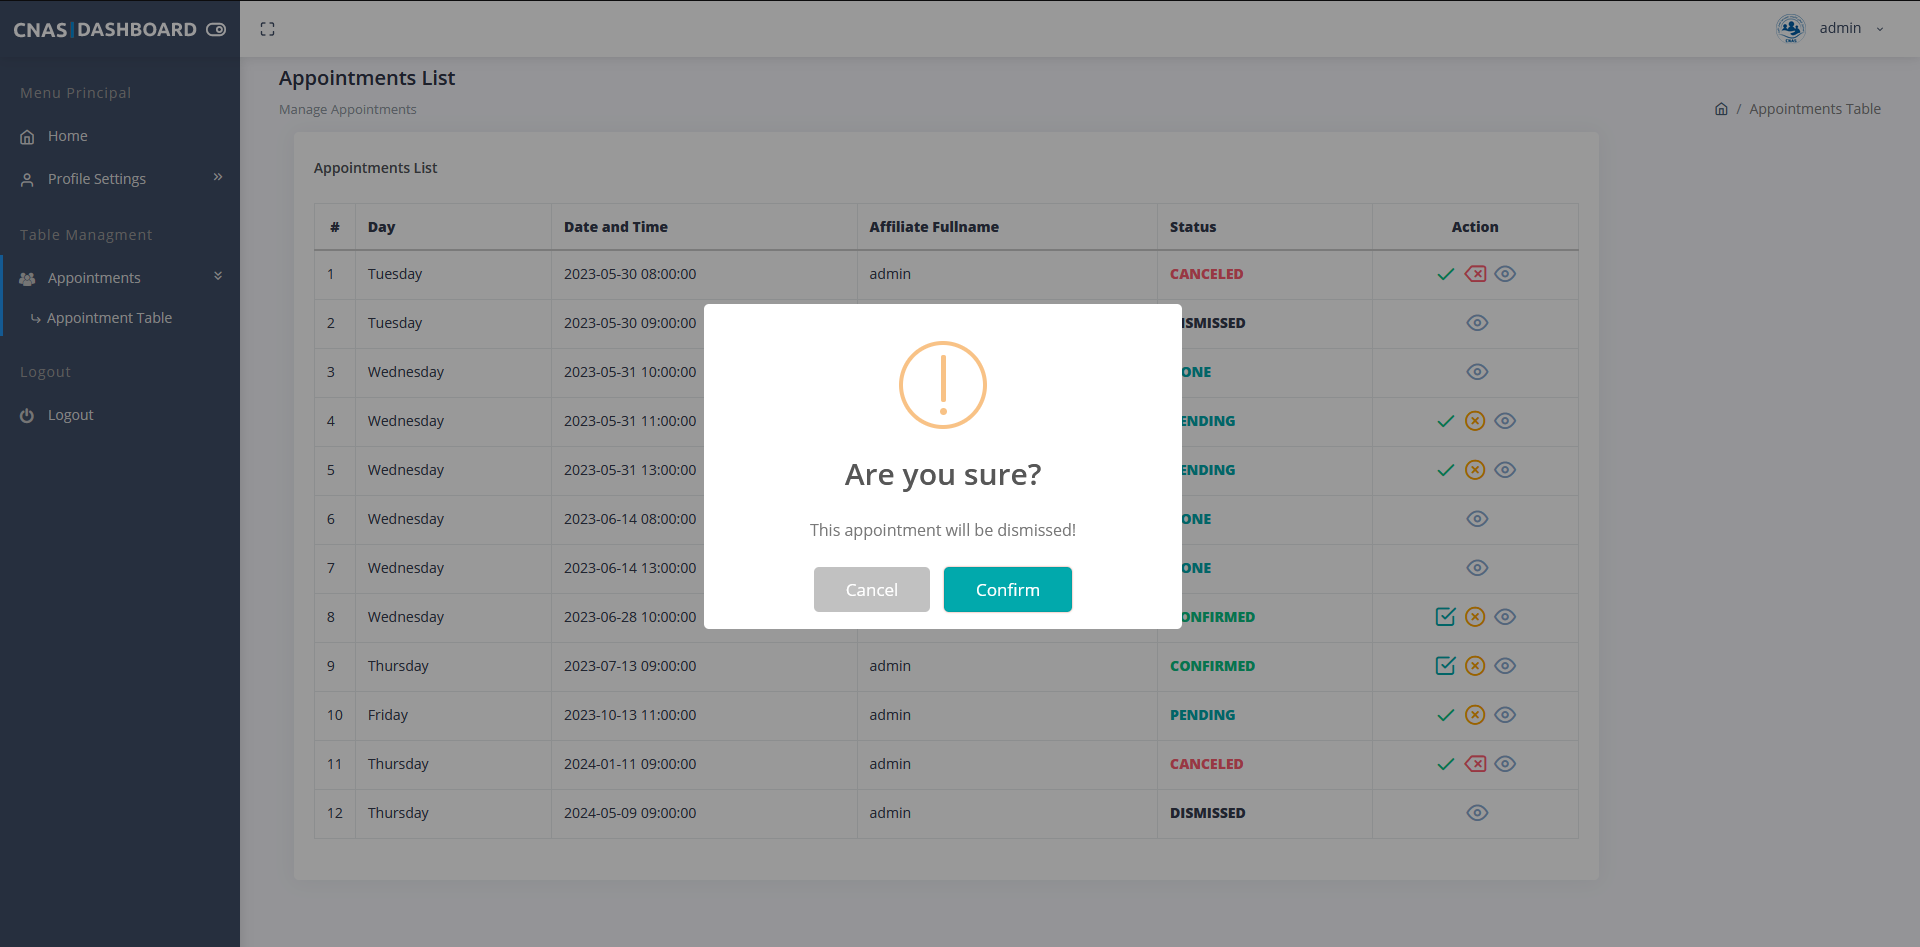
\includegraphics[width=0.7\textwidth]{SCREENSHOTS/admin/dismiss.png}
    \caption{Admin Appointment Dismiss}
    \label{fig:admin-appointment-dismiss}
\end{figure}
\paragraph{Comment:} The screenshot above showcases the admin's ability to dismiss an appointment but with caution.


\begin{figure}[htbp]
    \centering
    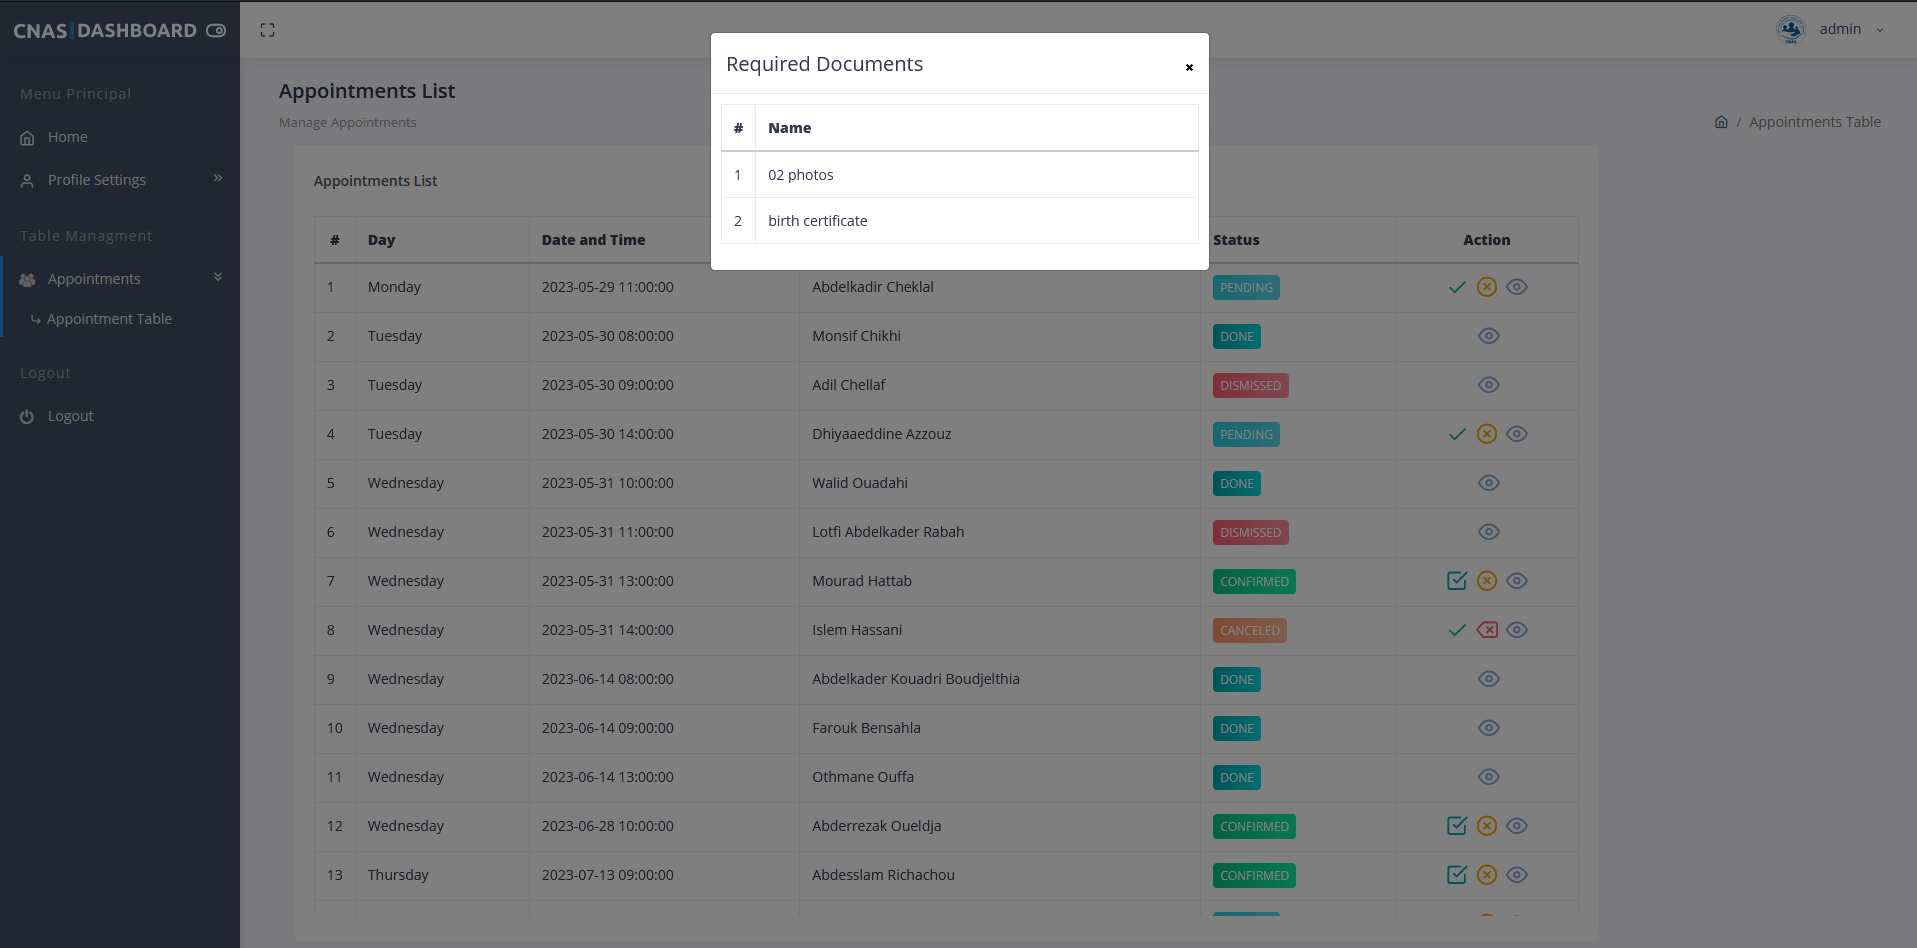
\includegraphics[width=0.7\textwidth]{SCREENSHOTS/admin/documents.png}
    \caption{Admin Appointment's Required Documents }
    \label{fig:admin-appointment-documents}
\end{figure}
\paragraph{Comment:} As shown above, the admin can see the documents that are required for the specific appointment.
\newpage
\end{itemize}

\newpage
\section{Conclusion}
In this chapter, we have explored the integration of Vue.js with Laravel and discussed its benefits in web development. Let's summarize the key points covered:
\begin{itemize}
    \item Vue.js is a progressive JavaScript framework known for its simplicity, reactivity, component-based architecture, and virtual DOM. It enables the creation of dynamic and interactive user interfaces.
    
    \item Understanding the fundamentals of Vue.js is essential, including components, which are reusable UI elements, and directives and templates, which define the structure and rendering of Vue components.

    \item Integrating Vue.js components into Laravel Blade templates allows you to leverage the power of Vue.js within your Laravel applications. You can share data between Laravel and Vue.js components using props and event handling, and build interactive UI elements that respond in real-time without the need for full-page reloads.

    \item The integration of Vue.js and Laravel brings several benefits. It enhances interactivity and responsiveness, improves the development experience, and promotes a separation of concerns between the front-end and back-end code. API-driven development enables efficient communication between the two layers, resulting in faster and more efficient applications.
\end{itemize}
In conclusion, the integration of Vue.js and Laravel opens up exciting possibilities for building modern and feature-rich web applications. By further exploring and learning these technologies, you can harness their full potential and unlock new opportunities for creativity and innovation in your development projects.

\addcontentsline{toc}{chapter}{Conclusion}
\chapter*{Conclusion}


\bibliography{references}
\bibliographystyle{ieeetr} 
\end{document}